\section*{Results}
\label{Results} 

Table~\ref{tab:regResults} displays the results from our model. To contrast with findings from the extant literature, we run the model in three ways. The first column tests the literature's explanations of sanction compliance centered on target state characteristics. In the second column, we add covariates to account for a target's relationships with sender states. The final model incorporates our reciprocity measures. 

% latex table generated in R 3.1.0 by xtable 1.7-3 package
% Sat Aug  2 12:32:14 2014
\begin{table}[ht]
\centering
{\normalsize
\begin{tabular}{lccc}
 Variable & Model 1 & Model 2 & Model 3 \\ 
  \hline
\hline
Compliance Reciprocity$_{j,t-1}$ &  &  & $0.212^{\ast\ast}$ \\ 
   &  &  & (0.063) \\ 
  Sanction Reciprocity$_{j,t-1}$ &  &  & $-0.103^{\ast\ast}$ \\ 
   &  &  & (0.033) \\ 
   \hline
Number of Senders$_{j,t}$ &  & $0.255^{\ast\ast}$ & $0.234^{\ast\ast}$ \\ 
   &  & (0.062) & (0.062) \\ 
  Distance$_{j,t}$ &  & $0.531^{\ast\ast}$ & $0.497^{\ast\ast}$ \\ 
   &  & (0.183) & (0.187) \\ 
  Trade$_{j,t}$ &  & $16.795^{\ast}$ & $16.106^{\ast}$ \\ 
   &  & (9.393) & (9.398) \\ 
  Ally$_{j,t}$ &  & 0.029 & 0.096 \\ 
   &  & (0.159) & (0.164) \\ 
   \hline
Polity$_{i,t-1}$ & $-0.029^{\ast}$ & -0.015 & -0.022 \\ 
   & (0.016) & (0.017) & (0.017) \\ 
  Ln(GDP per capita)$_{i,t-1}$ & -0.088 & -0.08 & -0.03 \\ 
   & (0.065) & (0.07) & (0.073) \\ 
  GDP Growth$_{i,t-1}$ & 0.011 & 0.02 & 0.015 \\ 
   & (0.018) & (0.019) & (0.019) \\ 
  Population$_{i,t-1}$ & $-0.172^{\ast\ast}$ & $-0.16^{\ast\ast}$ & $-0.102^{\ast\ast}$ \\ 
   & (0.039) & (0.043) & (0.05) \\ 
  Internal Conflict$_{i,t-1}$ & 0.001 & 0.004 & -0.001 \\ 
   & (0.017) & (0.017) & (0.017) \\ 
   \hline
n & 6517 & 6483 & 6483 \\ 
  Events & 191 & 190 & 190 \\ 
  Likelihood ratio test & 36.91 (0) & 59.55 (0) & 70.76 (0) \\ 
   \hline
\hline
\end{tabular}
}
\caption{Duration model with time varying covariates estimated using Cox Proportional Hazards. Standard errors in parentheses. $^{**}$ and $^{*}$ indicate significance at $p< 0.05 $ and $p< 0.10 $, respectively.} 
\label{tab:regResults}
\end{table}


We find no support for the argument that high levels of internal stability may prompt a country to comply. Across each specification, we find that countries with higher levels of GDP per capita take longer to comply to a sanction case, indicating that wealthier countries are able to resist complying to sanctions for lengthier durations. Additionally, like previous work in the literature, we find that more democratic countries are likely to take a shorter time to comply to sanctions. Because it is difficult to interpret the substantive meaning of point estimates from the hazard function in Table~\ref{tab:regResults}, we visualize Kaplan-Meier estimates of survival probabilities. The y-axis in these charts represents the probability of survival, or in this case the probability that a country will not comply to a sanction, and the x-axis represents time since sanction initiation (measured in years). The grey line represents the scenario where the number of senders variable is set to a low value, in this case one, and the black line represents the scenario where this variable is set to its high value, in this case five. All the other covariates were set to their median. Using these estimates, we trace the effect of GDP per capita and polity on the probability of sanction compliance as a function of time., the results are shown in Figure~\ref{fig:monSurv}. In the case of polity, we can see that its effect on the timing of sanction compliance is actually quite minimal. Even 15 years after sanction initiation, the difference in the probability of a completely democratic regime, polity score of 10, relative to a completely authoritarian regime, polity score of -10, complying to a sanction is only 15\%. The predicted difference in compliance probabilities between regimes of different GDP per capitas, however, is quite stark. Just five years after a sanction was initiated, extremely poor regimes are almost a coin's toss away from compliance, whereas well-off regimes are extremely unlikely to comply. 

\begin{figure}[ht]
	\centering
	\caption{Survival probabilities by ``proximity'' covariates. Grey designates scenarios in which the covariate is set to its minimum value and black where it is set to its maximum value.}
	% \begin{tabular}{cc}

    % \subfloat[SubFigure 1][Log(GDP per Capita)]{
        \resizebox{.55\textwidth}{!}{% Created by tikzDevice version 0.8.1 on 2015-05-24 13:12:08
% !TEX encoding = UTF-8 Unicode
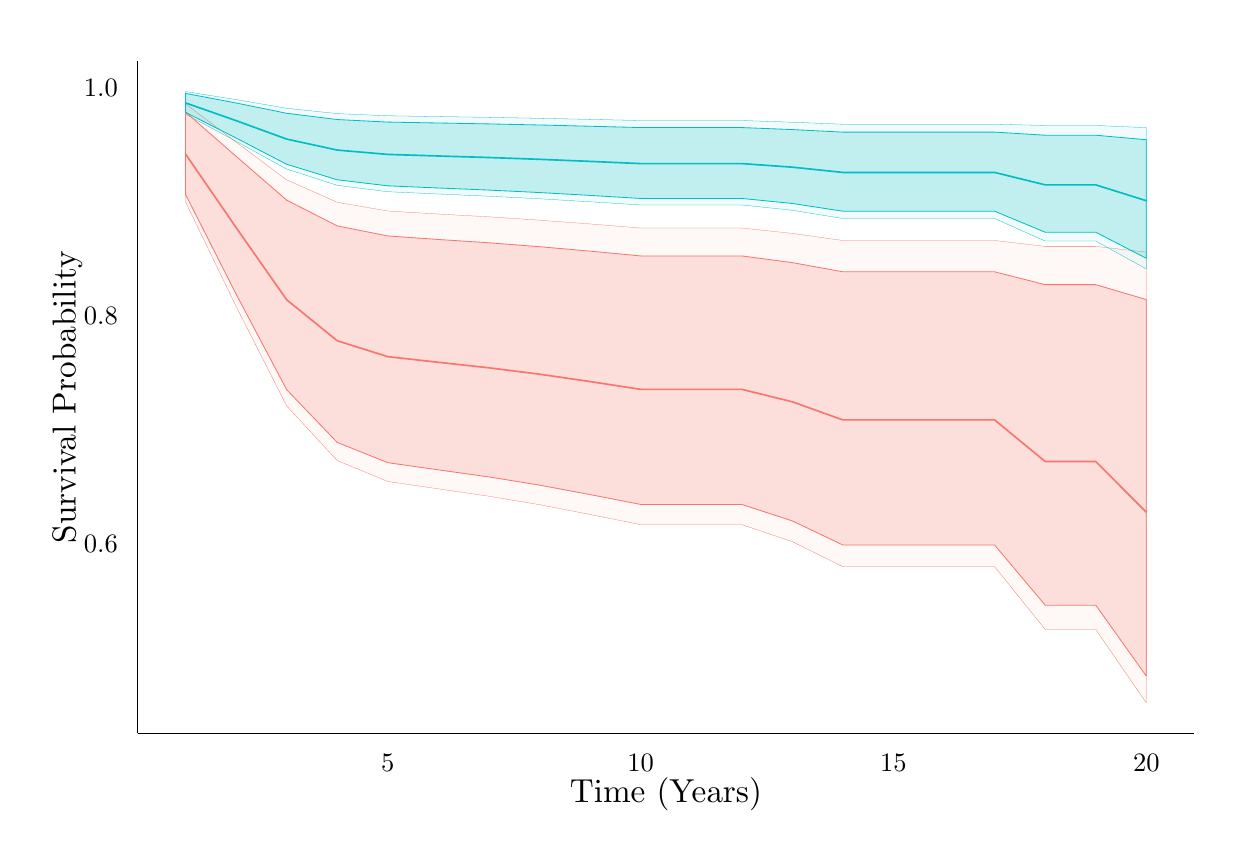
\begin{tikzpicture}[x=1pt,y=1pt]
\definecolor{fillColor}{RGB}{255,255,255}
\path[use as bounding box,fill=fillColor,fill opacity=0.00] (0,0) rectangle (433.62,289.08);
\begin{scope}
\path[clip] (  0.00,  0.00) rectangle (433.62,289.08);
\definecolor{drawColor}{RGB}{255,255,255}
\definecolor{fillColor}{RGB}{255,255,255}

\path[draw=drawColor,line width= 0.6pt,line join=round,line cap=round,fill=fillColor] (  0.00,  0.00) rectangle (433.62,289.08);
\end{scope}
\begin{scope}
\path[clip] ( 39.69, 34.03) rectangle (421.57,277.03);
\definecolor{fillColor}{RGB}{255,255,255}

\path[fill=fillColor] ( 39.69, 34.03) rectangle (421.58,277.03);
\definecolor{drawColor}{RGB}{248,118,109}

\path[draw=drawColor,line width= 0.6pt,line join=round] ( 57.05,243.40) --
	( 75.32,216.83) --
	( 93.59,190.76) --
	(111.86,175.94) --
	(130.13,170.20) --
	(148.41,168.16) --
	(166.68,166.17) --
	(184.95,163.86) --
	(203.22,161.20) --
	(221.49,158.39) --
	(239.77,158.39) --
	(258.04,158.39) --
	(276.31,153.88) --
	(294.58,147.34) --
	(312.86,147.34) --
	(331.13,147.34) --
	(349.40,147.34) --
	(367.67,132.31) --
	(385.94,132.31) --
	(404.22,113.99);
\definecolor{drawColor}{RGB}{0,191,196}

\path[draw=drawColor,line width= 0.6pt,line join=round] ( 57.05,261.89) --
	( 75.32,255.48) --
	( 93.59,248.82) --
	(111.86,244.85) --
	(130.13,243.28) --
	(148.41,242.71) --
	(166.68,242.16) --
	(184.95,241.51) --
	(203.22,240.76) --
	(221.49,239.96) --
	(239.77,239.96) --
	(258.04,239.96) --
	(276.31,238.67) --
	(294.58,236.77) --
	(312.86,236.77) --
	(331.13,236.77) --
	(349.40,236.77) --
	(367.67,232.28) --
	(385.94,232.28) --
	(404.22,226.54);
\definecolor{drawColor}{RGB}{248,118,109}
\definecolor{fillColor}{RGB}{248,118,109}

\path[draw=drawColor,line width= 0.1pt,line join=round,line cap=round,fill=fillColor,fill opacity=0.05] ( 57.05,261.55) --
	( 75.32,247.73) --
	( 93.59,234.09) --
	(111.86,225.99) --
	(130.13,222.84) --
	(148.41,221.73) --
	(166.68,220.73) --
	(184.95,219.52) --
	(203.22,218.16) --
	(221.49,216.68) --
	(239.77,216.68) --
	(258.04,216.68) --
	(276.31,214.74) --
	(294.58,212.17) --
	(312.86,212.17) --
	(331.13,212.17) --
	(349.40,212.17) --
	(367.67,210.05) --
	(385.94,210.05) --
	(404.22,207.96) --
	(404.22, 45.08) --
	(385.94, 71.63) --
	(367.67, 71.63) --
	(349.40, 94.30) --
	(331.13, 94.30) --
	(312.86, 94.30) --
	(294.58, 94.30) --
	(276.31,103.34) --
	(258.04,109.51) --
	(239.77,109.51) --
	(221.49,109.51) --
	(203.22,113.19) --
	(184.95,116.71) --
	(166.68,119.77) --
	(148.41,122.43) --
	(130.13,125.10) --
	(111.86,132.66) --
	( 93.59,152.39) --
	( 75.32,188.37) --
	( 57.05,226.06) --
	cycle;
\definecolor{drawColor}{RGB}{0,191,196}
\definecolor{fillColor}{RGB}{0,191,196}

\path[draw=drawColor,line width= 0.1pt,line join=round,line cap=round,fill=fillColor,fill opacity=0.05] ( 57.05,265.99) --
	( 75.32,263.09) --
	( 93.59,259.95) --
	(111.86,258.03) --
	(130.13,257.24) --
	(148.41,256.95) --
	(166.68,256.67) --
	(184.95,256.33) --
	(203.22,255.94) --
	(221.49,255.53) --
	(239.77,255.53) --
	(258.04,255.53) --
	(276.31,254.91) --
	(294.58,254.19) --
	(312.86,254.19) --
	(331.13,254.19) --
	(349.40,254.19) --
	(367.67,253.74) --
	(385.94,253.74) --
	(404.22,252.95) --
	(404.22,201.88) --
	(385.94,211.98) --
	(367.67,211.98) --
	(349.40,220.12) --
	(331.13,220.12) --
	(312.86,220.12) --
	(294.58,220.12) --
	(276.31,223.10) --
	(258.04,225.01) --
	(239.77,225.01) --
	(221.49,225.01) --
	(203.22,226.16) --
	(184.95,227.24) --
	(166.68,228.17) --
	(148.41,228.98) --
	(130.13,229.80) --
	(111.86,232.10) --
	( 93.59,237.99) --
	( 75.32,248.01) --
	( 57.05,257.84) --
	cycle;
\definecolor{drawColor}{RGB}{248,118,109}
\definecolor{fillColor}{RGB}{248,118,109}

\path[draw=drawColor,line width= 0.3pt,line join=round,line cap=round,fill=fillColor,fill opacity=0.20] ( 57.05,258.58) --
	( 75.32,242.59) --
	( 93.59,226.76) --
	(111.86,217.44) --
	(130.13,213.82) --
	(148.41,212.54) --
	(166.68,211.35) --
	(184.95,209.93) --
	(203.22,208.33) --
	(221.49,206.60) --
	(239.77,206.60) --
	(258.04,206.60) --
	(276.31,204.18) --
	(294.58,200.85) --
	(312.86,200.85) --
	(331.13,200.85) --
	(349.40,200.85) --
	(367.67,196.22) --
	(385.94,196.22) --
	(404.22,190.82) --
	(404.22, 54.77) --
	(385.94, 80.40) --
	(367.67, 80.40) --
	(349.40,102.13) --
	(331.13,102.13) --
	(312.86,102.13) --
	(294.58,102.13) --
	(276.31,110.85) --
	(258.04,116.80) --
	(239.77,116.80) --
	(221.49,116.80) --
	(203.22,120.36) --
	(184.95,123.78) --
	(166.68,126.74) --
	(148.41,129.30) --
	(130.13,131.89) --
	(111.86,139.20) --
	( 93.59,158.25) --
	( 75.32,192.79) --
	( 57.05,228.80) --
	cycle;
\definecolor{drawColor}{RGB}{0,191,196}
\definecolor{fillColor}{RGB}{0,191,196}

\path[draw=drawColor,line width= 0.3pt,line join=round,line cap=round,fill=fillColor,fill opacity=0.20] ( 57.05,265.33) --
	( 75.32,261.86) --
	( 93.59,258.14) --
	(111.86,255.88) --
	(130.13,254.96) --
	(148.41,254.63) --
	(166.68,254.30) --
	(184.95,253.91) --
	(203.22,253.46) --
	(221.49,252.98) --
	(239.77,252.98) --
	(258.04,252.98) --
	(276.31,252.25) --
	(294.58,251.33) --
	(312.86,251.33) --
	(331.13,251.33) --
	(349.40,251.33) --
	(367.67,250.21) --
	(385.94,250.21) --
	(404.22,248.58) --
	(404.22,205.73) --
	(385.94,215.17) --
	(367.67,215.17) --
	(349.40,222.75) --
	(331.13,222.75) --
	(312.86,222.75) --
	(294.58,222.75) --
	(276.31,225.56) --
	(258.04,227.37) --
	(239.77,227.37) --
	(221.49,227.37) --
	(203.22,228.47) --
	(184.95,229.50) --
	(166.68,230.39) --
	(148.41,231.15) --
	(130.13,231.93) --
	(111.86,234.12) --
	( 93.59,239.71) --
	( 75.32,249.20) --
	( 57.05,258.48) --
	cycle;
\end{scope}
\begin{scope}
\path[clip] (  0.00,  0.00) rectangle (433.62,289.08);
\definecolor{drawColor}{RGB}{0,0,0}

\path[draw=drawColor,line width= 0.6pt,line join=round] ( 39.69, 34.03) --
	( 39.69,277.03);
\end{scope}
\begin{scope}
\path[clip] (  0.00,  0.00) rectangle (433.62,289.08);
\definecolor{drawColor}{RGB}{0,0,0}

\node[text=drawColor,anchor=base east,inner sep=0pt, outer sep=0pt, scale=  0.96] at ( 32.57, 99.42) {0.6};

\node[text=drawColor,anchor=base east,inner sep=0pt, outer sep=0pt, scale=  0.96] at ( 32.57,181.75) {0.8};

\node[text=drawColor,anchor=base east,inner sep=0pt, outer sep=0pt, scale=  0.96] at ( 32.57,264.09) {1.0};
\end{scope}
\begin{scope}
\path[clip] (  0.00,  0.00) rectangle (433.62,289.08);
\definecolor{drawColor}{RGB}{0,0,0}

\path[draw=drawColor,line width= 0.6pt,line join=round] ( 39.69, 34.03) --
	(421.57, 34.03);
\end{scope}
\begin{scope}
\path[clip] (  0.00,  0.00) rectangle (433.62,289.08);
\definecolor{drawColor}{RGB}{0,0,0}

\node[text=drawColor,anchor=base,inner sep=0pt, outer sep=0pt, scale=  0.96] at (130.13, 20.31) {5};

\node[text=drawColor,anchor=base,inner sep=0pt, outer sep=0pt, scale=  0.96] at (221.49, 20.31) {10};

\node[text=drawColor,anchor=base,inner sep=0pt, outer sep=0pt, scale=  0.96] at (312.86, 20.31) {15};

\node[text=drawColor,anchor=base,inner sep=0pt, outer sep=0pt, scale=  0.96] at (404.22, 20.31) {20};
\end{scope}
\begin{scope}
\path[clip] (  0.00,  0.00) rectangle (433.62,289.08);
\definecolor{drawColor}{RGB}{0,0,0}

\node[text=drawColor,anchor=base,inner sep=0pt, outer sep=0pt, scale=  1.20] at (230.63,  9.03) {Time (Years)};
\end{scope}
\begin{scope}
\path[clip] (  0.00,  0.00) rectangle (433.62,289.08);
\definecolor{drawColor}{RGB}{0,0,0}

\node[text=drawColor,rotate= 90.00,anchor=base,inner sep=0pt, outer sep=0pt, scale=  1.20] at ( 17.30,155.53) {Survival Probability};
\end{scope}
\end{tikzpicture}
}	
        % \label{fig:gdpSurv}} & 

	% \subfloat[SubFigure 2][Polity]{
	% 	\resizebox{.45\textwidth}{!}{% Created by tikzDevice version 0.8.1 on 2015-05-24 13:12:07
% !TEX encoding = UTF-8 Unicode
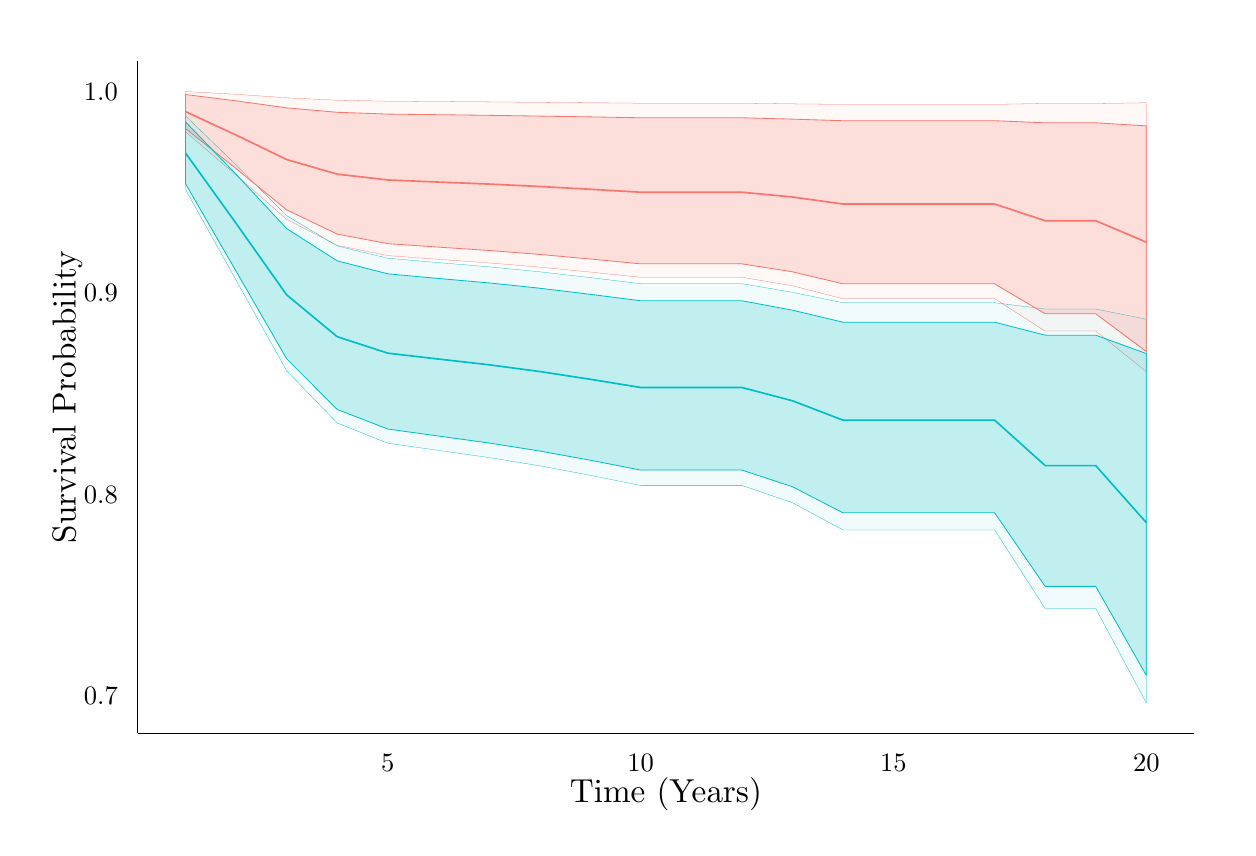
\begin{tikzpicture}[x=1pt,y=1pt]
\definecolor{fillColor}{RGB}{255,255,255}
\path[use as bounding box,fill=fillColor,fill opacity=0.00] (0,0) rectangle (433.62,289.08);
\begin{scope}
\path[clip] (  0.00,  0.00) rectangle (433.62,289.08);
\definecolor{drawColor}{RGB}{255,255,255}
\definecolor{fillColor}{RGB}{255,255,255}

\path[draw=drawColor,line width= 0.6pt,line join=round,line cap=round,fill=fillColor] (  0.00,  0.00) rectangle (433.62,289.08);
\end{scope}
\begin{scope}
\path[clip] ( 39.69, 34.03) rectangle (421.57,277.03);
\definecolor{fillColor}{RGB}{255,255,255}

\path[fill=fillColor] ( 39.69, 34.03) rectangle (421.58,277.03);
\definecolor{drawColor}{RGB}{248,118,109}

\path[draw=drawColor,line width= 0.6pt,line join=round] ( 57.05,258.74) --
	( 75.32,250.27) --
	( 93.59,241.43) --
	(111.86,236.15) --
	(130.13,234.05) --
	(148.41,233.29) --
	(166.68,232.56) --
	(184.95,231.69) --
	(203.22,230.69) --
	(221.49,229.62) --
	(239.77,229.62) --
	(258.04,229.62) --
	(276.31,227.90) --
	(294.58,225.35) --
	(312.86,225.35) --
	(331.13,225.35) --
	(349.40,225.35) --
	(367.67,219.32) --
	(385.94,219.32) --
	(404.22,211.58);
\definecolor{drawColor}{RGB}{0,191,196}

\path[draw=drawColor,line width= 0.6pt,line join=round] ( 57.05,243.76) --
	( 75.32,218.35) --
	( 93.59,192.52) --
	(111.86,177.41) --
	(130.13,171.46) --
	(148.41,169.34) --
	(166.68,167.26) --
	(184.95,164.84) --
	(203.22,162.04) --
	(221.49,159.07) --
	(239.77,159.07) --
	(258.04,159.07) --
	(276.31,154.27) --
	(294.58,147.26) --
	(312.86,147.26) --
	(331.13,147.26) --
	(349.40,147.26) --
	(367.67,130.84) --
	(385.94,130.84) --
	(404.22,110.22);
\definecolor{drawColor}{RGB}{248,118,109}
\definecolor{fillColor}{RGB}{248,118,109}

\path[draw=drawColor,line width= 0.1pt,line join=round,line cap=round,fill=fillColor,fill opacity=0.05] ( 57.05,265.99) --
	( 75.32,265.02) --
	( 93.59,263.74) --
	(111.86,262.86) --
	(130.13,262.51) --
	(148.41,262.39) --
	(166.68,262.26) --
	(184.95,262.11) --
	(203.22,261.96) --
	(221.49,261.79) --
	(239.77,261.79) --
	(258.04,261.79) --
	(276.31,261.55) --
	(294.58,261.37) --
	(312.86,261.37) --
	(331.13,261.37) --
	(349.40,261.37) --
	(367.67,261.68) --
	(385.94,261.68) --
	(404.22,261.93) --
	(404.22,164.75) --
	(385.94,179.44) --
	(367.67,179.44) --
	(349.40,191.13) --
	(331.13,191.13) --
	(312.86,191.13) --
	(294.58,191.13) --
	(276.31,195.81) --
	(258.04,198.89) --
	(239.77,198.89) --
	(221.49,198.89) --
	(203.22,200.77) --
	(184.95,202.55) --
	(166.68,204.07) --
	(148.41,205.37) --
	(130.13,206.71) --
	(111.86,210.42) --
	( 93.59,219.80) --
	( 75.32,235.81) --
	( 57.05,251.44) --
	cycle;
\definecolor{drawColor}{RGB}{0,191,196}
\definecolor{fillColor}{RGB}{0,191,196}

\path[draw=drawColor,line width= 0.1pt,line join=round,line cap=round,fill=fillColor,fill opacity=0.05] ( 57.05,257.18) --
	( 75.32,239.53) --
	( 93.59,221.15) --
	(111.86,210.20) --
	(130.13,205.77) --
	(148.41,204.18) --
	(166.68,202.68) --
	(184.95,200.86) --
	(203.22,198.78) --
	(221.49,196.58) --
	(239.77,196.58) --
	(258.04,196.58) --
	(276.31,193.47) --
	(294.58,189.68) --
	(312.86,189.68) --
	(331.13,189.68) --
	(349.40,189.68) --
	(367.67,187.41) --
	(385.94,187.41) --
	(404.22,183.74) --
	(404.22, 45.08) --
	(385.94, 79.19) --
	(367.67, 79.19) --
	(349.40,107.60) --
	(331.13,107.60) --
	(312.86,107.60) --
	(294.58,107.60) --
	(276.31,117.43) --
	(258.04,123.69) --
	(239.77,123.69) --
	(221.49,123.69) --
	(203.22,127.34) --
	(184.95,130.77) --
	(166.68,133.74) --
	(148.41,136.33) --
	(130.13,138.92) --
	(111.86,146.22) --
	( 93.59,165.09) --
	( 75.32,197.80) --
	( 57.05,230.58) --
	cycle;
\definecolor{drawColor}{RGB}{248,118,109}
\definecolor{fillColor}{RGB}{248,118,109}

\path[draw=drawColor,line width= 0.3pt,line join=round,line cap=round,fill=fillColor,fill opacity=0.20] ( 57.05,264.92) --
	( 75.32,262.63) --
	( 93.59,260.11) --
	(111.86,258.50) --
	(130.13,257.85) --
	(148.41,257.63) --
	(166.68,257.40) --
	(184.95,257.13) --
	(203.22,256.84) --
	(221.49,256.52) --
	(239.77,256.52) --
	(258.04,256.52) --
	(276.31,256.03) --
	(294.58,255.45) --
	(312.86,255.45) --
	(331.13,255.45) --
	(349.40,255.45) --
	(367.67,254.70) --
	(385.94,254.70) --
	(404.22,253.59) --
	(404.22,172.05) --
	(385.94,185.69) --
	(367.67,185.69) --
	(349.40,196.52) --
	(331.13,196.52) --
	(312.86,196.52) --
	(294.58,196.52) --
	(276.31,200.87) --
	(258.04,203.74) --
	(239.77,203.74) --
	(221.49,203.74) --
	(203.22,205.49) --
	(184.95,207.15) --
	(166.68,208.57) --
	(148.41,209.78) --
	(130.13,211.03) --
	(111.86,214.50) --
	( 93.59,223.23) --
	( 75.32,238.12) --
	( 57.05,252.61) --
	cycle;
\definecolor{drawColor}{RGB}{0,191,196}
\definecolor{fillColor}{RGB}{0,191,196}

\path[draw=drawColor,line width= 0.3pt,line join=round,line cap=round,fill=fillColor,fill opacity=0.20] ( 57.05,255.00) --
	( 75.32,236.08) --
	( 93.59,216.47) --
	(111.86,204.82) --
	(130.13,200.13) --
	(148.41,198.45) --
	(166.68,196.85) --
	(184.95,194.94) --
	(203.22,192.73) --
	(221.49,190.40) --
	(239.77,190.40) --
	(258.04,190.40) --
	(276.31,187.00) --
	(294.58,182.66) --
	(312.86,182.66) --
	(331.13,182.66) --
	(349.40,182.66) --
	(367.67,177.96) --
	(385.94,177.96) --
	(404.22,171.31) --
	(404.22, 55.03) --
	(385.94, 87.18) --
	(367.67, 87.18) --
	(349.40,113.79) --
	(331.13,113.79) --
	(312.86,113.79) --
	(294.58,113.79) --
	(276.31,123.20) --
	(258.04,129.24) --
	(239.77,129.24) --
	(221.49,129.24) --
	(203.22,132.79) --
	(184.95,136.12) --
	(166.68,139.01) --
	(148.41,141.52) --
	(130.13,144.04) --
	(111.86,151.13) --
	( 93.59,169.42) --
	( 75.32,201.06) --
	( 57.05,232.68) --
	cycle;
\end{scope}
\begin{scope}
\path[clip] (  0.00,  0.00) rectangle (433.62,289.08);
\definecolor{drawColor}{RGB}{0,0,0}

\path[draw=drawColor,line width= 0.6pt,line join=round] ( 39.69, 34.03) --
	( 39.69,277.03);
\end{scope}
\begin{scope}
\path[clip] (  0.00,  0.00) rectangle (433.62,289.08);
\definecolor{drawColor}{RGB}{0,0,0}

\node[text=drawColor,anchor=base east,inner sep=0pt, outer sep=0pt, scale=  0.96] at ( 32.57, 44.50) {0.7};

\node[text=drawColor,anchor=base east,inner sep=0pt, outer sep=0pt, scale=  0.96] at ( 32.57,117.23) {0.8};

\node[text=drawColor,anchor=base east,inner sep=0pt, outer sep=0pt, scale=  0.96] at ( 32.57,189.96) {0.9};

\node[text=drawColor,anchor=base east,inner sep=0pt, outer sep=0pt, scale=  0.96] at ( 32.57,262.68) {1.0};
\end{scope}
\begin{scope}
\path[clip] (  0.00,  0.00) rectangle (433.62,289.08);
\definecolor{drawColor}{RGB}{0,0,0}

\path[draw=drawColor,line width= 0.6pt,line join=round] ( 39.69, 34.03) --
	(421.57, 34.03);
\end{scope}
\begin{scope}
\path[clip] (  0.00,  0.00) rectangle (433.62,289.08);
\definecolor{drawColor}{RGB}{0,0,0}

\node[text=drawColor,anchor=base,inner sep=0pt, outer sep=0pt, scale=  0.96] at (130.13, 20.31) {5};

\node[text=drawColor,anchor=base,inner sep=0pt, outer sep=0pt, scale=  0.96] at (221.49, 20.31) {10};

\node[text=drawColor,anchor=base,inner sep=0pt, outer sep=0pt, scale=  0.96] at (312.86, 20.31) {15};

\node[text=drawColor,anchor=base,inner sep=0pt, outer sep=0pt, scale=  0.96] at (404.22, 20.31) {20};
\end{scope}
\begin{scope}
\path[clip] (  0.00,  0.00) rectangle (433.62,289.08);
\definecolor{drawColor}{RGB}{0,0,0}

\node[text=drawColor,anchor=base,inner sep=0pt, outer sep=0pt, scale=  1.20] at (230.63,  9.03) {Time (Years)};
\end{scope}
\begin{scope}
\path[clip] (  0.00,  0.00) rectangle (433.62,289.08);
\definecolor{drawColor}{RGB}{0,0,0}

\node[text=drawColor,rotate= 90.00,anchor=base,inner sep=0pt, outer sep=0pt, scale=  1.20] at ( 17.30,155.53) {Survival Probability};
\end{scope}
\end{tikzpicture}
}	
	% 	\label{fig:polSurv}}

	% \end{tabular}
	
	\label{fig:monSurv}
\end{figure}


We also find strong support for the argument that states are more likely to comply to sanctions involving multiple actors, and the effect of this variable remains consistent even after controlling for our network level covariates in Model 3. Using Figure~\ref{fig:nosSurv} we can quickly see that there is a stark difference in the likelihood of non-compliance between a sanction case involving single and multiple senders. After just five years the probability of non-compliance drops to approximately 60\%, whereas a sanction from a single sender by that time still has almost a 95\% chance of non-compliance. This finding is in sharp contrast to previous research arguing that multilateral sanctions can actually be counterproductive.\footnote{For example, see \citealp{drezner2000bargaining}.} Unlike the extant literature, we do not find strong evidence for the ability of trading partners to obtain quick and successful resolutions to sanction cases. States are also not likely to comply more quickly to sanctions sent by allies, and are actually less likely to comply to neighbors. 

\begin{figure}[ht]
	\centering
	\caption{Survival probabilities reflecting variation in the number of senders in a sanction case. Grey designates the scenario where the number of senders is set to its minimum value and black the scenario where it is set to its high value (90th percentile).}
	% \includegraphics[width=1\textwidth]{nosSurv}
	\resizebox{0.55\textwidth}{!}{% Created by tikzDevice version 0.8.1 on 2015-05-16 17:34:47
% !TEX encoding = UTF-8 Unicode
\begin{tikzpicture}[x=1pt,y=1pt]
\definecolor{fillColor}{RGB}{255,255,255}
\path[use as bounding box,fill=fillColor,fill opacity=0.00] (0,0) rectangle (433.62,289.08);
\begin{scope}
\path[clip] (  0.00,  0.00) rectangle (433.62,289.08);
\definecolor{drawColor}{RGB}{0,0,0}

\path[draw=drawColor,line width= 0.4pt,line join=round,line cap=round] ( 49.20, 61.20) -- (408.42, 61.20);

\path[draw=drawColor,line width= 0.4pt,line join=round,line cap=round] ( 49.20, 61.20) -- ( 49.20, 55.20);

\path[draw=drawColor,line width= 0.4pt,line join=round,line cap=round] (109.07, 61.20) -- (109.07, 55.20);

\path[draw=drawColor,line width= 0.4pt,line join=round,line cap=round] (168.94, 61.20) -- (168.94, 55.20);

\path[draw=drawColor,line width= 0.4pt,line join=round,line cap=round] (228.81, 61.20) -- (228.81, 55.20);

\path[draw=drawColor,line width= 0.4pt,line join=round,line cap=round] (288.68, 61.20) -- (288.68, 55.20);

\path[draw=drawColor,line width= 0.4pt,line join=round,line cap=round] (348.55, 61.20) -- (348.55, 55.20);

\path[draw=drawColor,line width= 0.4pt,line join=round,line cap=round] (408.42, 61.20) -- (408.42, 55.20);

\node[text=drawColor,anchor=base,inner sep=0pt, outer sep=0pt, scale=  1.00] at ( 49.20, 39.60) {0};

\node[text=drawColor,anchor=base,inner sep=0pt, outer sep=0pt, scale=  1.00] at (109.07, 39.60) {5};

\node[text=drawColor,anchor=base,inner sep=0pt, outer sep=0pt, scale=  1.00] at (168.94, 39.60) {10};

\node[text=drawColor,anchor=base,inner sep=0pt, outer sep=0pt, scale=  1.00] at (228.81, 39.60) {15};

\node[text=drawColor,anchor=base,inner sep=0pt, outer sep=0pt, scale=  1.00] at (288.68, 39.60) {20};

\node[text=drawColor,anchor=base,inner sep=0pt, outer sep=0pt, scale=  1.00] at (348.55, 39.60) {25};

\node[text=drawColor,anchor=base,inner sep=0pt, outer sep=0pt, scale=  1.00] at (408.42, 39.60) {30};

\path[draw=drawColor,line width= 0.4pt,line join=round,line cap=round] ( 49.20, 67.82) -- ( 49.20,233.26);

\path[draw=drawColor,line width= 0.4pt,line join=round,line cap=round] ( 49.20, 67.82) -- ( 43.20, 67.82);

\path[draw=drawColor,line width= 0.4pt,line join=round,line cap=round] ( 49.20,109.18) -- ( 43.20,109.18);

\path[draw=drawColor,line width= 0.4pt,line join=round,line cap=round] ( 49.20,150.54) -- ( 43.20,150.54);

\path[draw=drawColor,line width= 0.4pt,line join=round,line cap=round] ( 49.20,191.90) -- ( 43.20,191.90);

\path[draw=drawColor,line width= 0.4pt,line join=round,line cap=round] ( 49.20,233.26) -- ( 43.20,233.26);

\node[text=drawColor,anchor=base east,inner sep=0pt, outer sep=0pt, scale=  1.00] at ( 37.20, 64.37) {0.2};

\node[text=drawColor,anchor=base east,inner sep=0pt, outer sep=0pt, scale=  1.00] at ( 37.20,105.74) {0.4};

\node[text=drawColor,anchor=base east,inner sep=0pt, outer sep=0pt, scale=  1.00] at ( 37.20,147.10) {0.6};

\node[text=drawColor,anchor=base east,inner sep=0pt, outer sep=0pt, scale=  1.00] at ( 37.20,188.46) {0.8};

\node[text=drawColor,anchor=base east,inner sep=0pt, outer sep=0pt, scale=  1.00] at ( 37.20,229.82) {1.0};
\end{scope}
\begin{scope}
\path[clip] (  0.00,  0.00) rectangle (433.62,289.08);
\definecolor{drawColor}{RGB}{0,0,0}

\node[text=drawColor,anchor=base,inner sep=0pt, outer sep=0pt, scale=  1.00] at (228.81, 15.60) {Time (Years)};

\node[text=drawColor,rotate= 90.00,anchor=base,inner sep=0pt, outer sep=0pt, scale=  1.00] at ( 10.80,150.54) {Survival Probability};
\end{scope}
\begin{scope}
\path[clip] ( 49.20, 61.20) rectangle (408.42,239.88);
\definecolor{drawColor}{RGB}{169,169,169}

\path[draw=drawColor,line width= 0.4pt,line join=round,line cap=round] ( 49.20,233.26) --
	( 61.17,233.26) --
	( 61.17,229.01) --
	( 73.15,229.01) --
	( 73.15,224.14) --
	( 85.12,224.14) --
	( 85.12,218.85) --
	( 97.10,218.85) --
	( 97.10,215.94) --
	(109.07,215.94) --
	(109.07,214.09) --
	(121.04,214.09) --
	(121.04,213.30) --
	(133.02,213.30) --
	(133.02,212.92) --
	(144.99,212.92) --
	(144.99,212.50) --
	(156.97,212.50) --
	(156.97,212.03) --
	(168.94,212.03) --
	(168.94,211.56) --
	(180.91,211.56) --
	(180.91,211.05) --
	(204.86,211.05) --
	(204.86,210.45) --
	(216.84,210.45) --
	(216.84,209.80) --
	(252.76,209.80) --
	(252.76,208.69) --
	(264.73,208.69) --
	(264.73,206.89) --
	(288.68,206.89) --
	(288.68,203.45) --
	(300.65,203.45) --
	(300.65,199.35) --
	(336.58,199.35) --
	(336.58,195.48) --
	(433.62,195.48);

\path[draw=drawColor,line width= 0.4pt,line join=round,line cap=round] ( 57.99,229.01) -- ( 64.36,229.01);

\path[draw=drawColor,line width= 0.4pt,line join=round,line cap=round] ( 61.17,225.83) -- ( 61.17,232.19);

\path[draw=drawColor,line width= 0.4pt,line join=round,line cap=round] ( 69.97,224.14) -- ( 76.33,224.14);

\path[draw=drawColor,line width= 0.4pt,line join=round,line cap=round] ( 73.15,220.95) -- ( 73.15,227.32);

\path[draw=drawColor,line width= 0.4pt,line join=round,line cap=round] ( 81.94,218.85) -- ( 88.30,218.85);

\path[draw=drawColor,line width= 0.4pt,line join=round,line cap=round] ( 85.12,215.67) -- ( 85.12,222.03);

\path[draw=drawColor,line width= 0.4pt,line join=round,line cap=round] ( 93.91,215.94) -- (100.28,215.94);

\path[draw=drawColor,line width= 0.4pt,line join=round,line cap=round] ( 97.10,212.76) -- ( 97.10,219.12);

\path[draw=drawColor,line width= 0.4pt,line join=round,line cap=round] (105.89,214.09) -- (112.25,214.09);

\path[draw=drawColor,line width= 0.4pt,line join=round,line cap=round] (109.07,210.91) -- (109.07,217.27);

\path[draw=drawColor,line width= 0.4pt,line join=round,line cap=round] (117.86,213.30) -- (124.23,213.30);

\path[draw=drawColor,line width= 0.4pt,line join=round,line cap=round] (121.04,210.12) -- (121.04,216.49);

\path[draw=drawColor,line width= 0.4pt,line join=round,line cap=round] (129.84,212.92) -- (136.20,212.92);

\path[draw=drawColor,line width= 0.4pt,line join=round,line cap=round] (133.02,209.74) -- (133.02,216.10);

\path[draw=drawColor,line width= 0.4pt,line join=round,line cap=round] (141.81,212.50) -- (148.17,212.50);

\path[draw=drawColor,line width= 0.4pt,line join=round,line cap=round] (144.99,209.32) -- (144.99,215.68);

\path[draw=drawColor,line width= 0.4pt,line join=round,line cap=round] (153.78,212.03) -- (160.15,212.03);

\path[draw=drawColor,line width= 0.4pt,line join=round,line cap=round] (156.97,208.85) -- (156.97,215.21);

\path[draw=drawColor,line width= 0.4pt,line join=round,line cap=round] (165.76,211.56) -- (172.12,211.56);

\path[draw=drawColor,line width= 0.4pt,line join=round,line cap=round] (168.94,208.38) -- (168.94,214.74);

\path[draw=drawColor,line width= 0.4pt,line join=round,line cap=round] (177.73,211.05) -- (184.10,211.05);

\path[draw=drawColor,line width= 0.4pt,line join=round,line cap=round] (180.91,207.87) -- (180.91,214.24);

\path[draw=drawColor,line width= 0.4pt,line join=round,line cap=round] (189.71,211.05) -- (196.07,211.05);

\path[draw=drawColor,line width= 0.4pt,line join=round,line cap=round] (192.89,207.87) -- (192.89,214.24);

\path[draw=drawColor,line width= 0.4pt,line join=round,line cap=round] (201.68,210.45) -- (208.04,210.45);

\path[draw=drawColor,line width= 0.4pt,line join=round,line cap=round] (204.86,207.27) -- (204.86,213.63);

\path[draw=drawColor,line width= 0.4pt,line join=round,line cap=round] (213.65,209.80) -- (220.02,209.80);

\path[draw=drawColor,line width= 0.4pt,line join=round,line cap=round] (216.84,206.62) -- (216.84,212.98);

\path[draw=drawColor,line width= 0.4pt,line join=round,line cap=round] (225.63,209.80) -- (231.99,209.80);

\path[draw=drawColor,line width= 0.4pt,line join=round,line cap=round] (228.81,206.62) -- (228.81,212.98);

\path[draw=drawColor,line width= 0.4pt,line join=round,line cap=round] (237.60,209.80) -- (243.97,209.80);

\path[draw=drawColor,line width= 0.4pt,line join=round,line cap=round] (240.78,206.62) -- (240.78,212.98);

\path[draw=drawColor,line width= 0.4pt,line join=round,line cap=round] (249.58,208.69) -- (255.94,208.69);

\path[draw=drawColor,line width= 0.4pt,line join=round,line cap=round] (252.76,205.51) -- (252.76,211.87);

\path[draw=drawColor,line width= 0.4pt,line join=round,line cap=round] (261.55,206.89) -- (267.91,206.89);

\path[draw=drawColor,line width= 0.4pt,line join=round,line cap=round] (264.73,203.71) -- (264.73,210.08);

\path[draw=drawColor,line width= 0.4pt,line join=round,line cap=round] (273.52,206.89) -- (279.89,206.89);

\path[draw=drawColor,line width= 0.4pt,line join=round,line cap=round] (276.71,203.71) -- (276.71,210.08);

\path[draw=drawColor,line width= 0.4pt,line join=round,line cap=round] (285.50,203.45) -- (291.86,203.45);

\path[draw=drawColor,line width= 0.4pt,line join=round,line cap=round] (288.68,200.27) -- (288.68,206.63);

\path[draw=drawColor,line width= 0.4pt,line join=round,line cap=round] (297.47,199.35) -- (303.84,199.35);

\path[draw=drawColor,line width= 0.4pt,line join=round,line cap=round] (300.65,196.17) -- (300.65,202.53);

\path[draw=drawColor,line width= 0.4pt,line join=round,line cap=round] (309.45,199.35) -- (315.81,199.35);

\path[draw=drawColor,line width= 0.4pt,line join=round,line cap=round] (312.63,196.17) -- (312.63,202.53);

\path[draw=drawColor,line width= 0.4pt,line join=round,line cap=round] (321.42,199.35) -- (327.78,199.35);

\path[draw=drawColor,line width= 0.4pt,line join=round,line cap=round] (324.60,196.17) -- (324.60,202.53);

\path[draw=drawColor,line width= 0.4pt,line join=round,line cap=round] (333.39,195.48) -- (339.76,195.48);

\path[draw=drawColor,line width= 0.4pt,line join=round,line cap=round] (336.58,192.30) -- (336.58,198.66);

\path[draw=drawColor,line width= 0.4pt,line join=round,line cap=round] (345.37,195.48) -- (351.73,195.48);

\path[draw=drawColor,line width= 0.4pt,line join=round,line cap=round] (348.55,192.30) -- (348.55,198.66);

\path[draw=drawColor,line width= 0.4pt,line join=round,line cap=round] (357.34,195.48) -- (363.71,195.48);

\path[draw=drawColor,line width= 0.4pt,line join=round,line cap=round] (360.52,192.30) -- (360.52,198.66);

\path[draw=drawColor,line width= 0.4pt,line join=round,line cap=round] (369.32,195.48) -- (375.68,195.48);

\path[draw=drawColor,line width= 0.4pt,line join=round,line cap=round] (372.50,192.30) -- (372.50,198.66);

\path[draw=drawColor,line width= 0.4pt,line join=round,line cap=round] (381.29,195.48) -- (387.65,195.48);

\path[draw=drawColor,line width= 0.4pt,line join=round,line cap=round] (384.47,192.30) -- (384.47,198.66);

\path[draw=drawColor,line width= 0.4pt,line join=round,line cap=round] (393.26,195.48) -- (399.63,195.48);

\path[draw=drawColor,line width= 0.4pt,line join=round,line cap=round] (396.45,192.30) -- (396.45,198.66);

\path[draw=drawColor,line width= 0.4pt,line join=round,line cap=round] (405.24,195.48) -- (411.60,195.48);

\path[draw=drawColor,line width= 0.4pt,line join=round,line cap=round] (408.42,192.30) -- (408.42,198.66);

\path[draw=drawColor,line width= 0.4pt,line join=round,line cap=round] (417.21,195.48) -- (423.58,195.48);

\path[draw=drawColor,line width= 0.4pt,line join=round,line cap=round] (420.39,192.30) -- (420.39,198.66);

\path[draw=drawColor,line width= 0.4pt,line join=round,line cap=round] (429.19,195.48) -- (433.62,195.48);

\path[draw=drawColor,line width= 0.4pt,line join=round,line cap=round] (432.37,192.30) -- (432.37,198.66);

\path[draw=drawColor,line width= 0.4pt,dash pattern=on 4pt off 4pt ,line join=round,line cap=round] ( 49.20,233.26) --
	( 61.17,233.26) --
	( 61.17,226.45) --
	( 73.15,226.45) --
	( 73.15,220.05) --
	( 85.12,220.05) --
	( 85.12,213.23) --
	( 97.10,213.23) --
	( 97.10,209.55) --
	(109.07,209.55) --
	(109.07,207.24) --
	(121.04,207.24) --
	(121.04,206.27) --
	(133.02,206.27) --
	(133.02,205.79) --
	(144.99,205.79) --
	(144.99,205.27) --
	(156.97,205.27) --
	(156.97,204.69) --
	(168.94,204.69) --
	(168.94,204.11) --
	(180.91,204.11) --
	(180.91,203.48) --
	(204.86,203.48) --
	(204.86,202.74) --
	(216.84,202.74) --
	(216.84,201.94) --
	(252.76,201.94) --
	(252.76,200.45) --
	(264.73,200.45) --
	(264.73,197.84) --
	(288.68,197.84) --
	(288.68,192.13) --
	(300.65,192.13) --
	(300.65,185.35) --
	(336.58,185.35) --
	(336.58,179.19) --
	(433.62,179.19);

\path[draw=drawColor,line width= 0.4pt,dash pattern=on 4pt off 4pt ,line join=round,line cap=round] ( 49.20,233.26) --
	( 61.17,233.26) --
	( 61.17,231.60) --
	( 73.15,231.60) --
	( 73.15,228.31) --
	( 85.12,228.31) --
	( 85.12,224.64) --
	( 97.10,224.64) --
	( 97.10,222.56) --
	(109.07,222.56) --
	(109.07,221.20) --
	(121.04,221.20) --
	(121.04,220.62) --
	(133.02,220.62) --
	(133.02,220.34) --
	(144.99,220.34) --
	(144.99,220.02) --
	(156.97,220.02) --
	(156.97,219.67) --
	(168.94,219.67) --
	(168.94,219.32) --
	(180.91,219.32) --
	(180.91,218.95) --
	(204.86,218.95) --
	(204.86,218.50) --
	(216.84,218.50) --
	(216.84,218.02) --
	(252.76,218.02) --
	(252.76,217.32) --
	(264.73,217.32) --
	(264.73,216.43) --
	(288.68,216.43) --
	(288.68,215.55) --
	(300.65,215.55) --
	(300.65,214.59) --
	(336.58,214.59) --
	(336.58,213.50) --
	(433.62,213.50);
\definecolor{drawColor}{RGB}{0,0,0}

\path[draw=drawColor,line width= 0.4pt,line join=round,line cap=round] ( 49.20,233.26) --
	( 61.17,233.26) --
	( 61.17,216.17) --
	( 73.15,216.17) --
	( 73.15,197.92) --
	( 85.12,197.92) --
	( 85.12,179.68) --
	( 97.10,179.68) --
	( 97.10,170.29) --
	(109.07,170.29) --
	(109.07,164.54) --
	(121.04,164.54) --
	(121.04,162.15) --
	(133.02,162.15) --
	(133.02,161.00) --
	(144.99,161.00) --
	(144.99,159.74) --
	(156.97,159.74) --
	(156.97,158.35) --
	(168.94,158.35) --
	(168.94,156.97) --
	(180.91,156.97) --
	(180.91,155.49) --
	(204.86,155.49) --
	(204.86,153.75) --
	(216.84,153.75) --
	(216.84,151.90) --
	(252.76,151.90) --
	(252.76,148.77) --
	(264.73,148.77) --
	(264.73,143.84) --
	(288.68,143.84) --
	(288.68,134.82) --
	(300.65,134.82) --
	(300.65,124.77) --
	(336.58,124.77) --
	(336.58,115.95) --
	(433.62,115.95);

\path[draw=drawColor,line width= 0.4pt,line join=round,line cap=round] ( 57.99,216.17) -- ( 64.36,216.17);

\path[draw=drawColor,line width= 0.4pt,line join=round,line cap=round] ( 61.17,212.99) -- ( 61.17,219.35);

\path[draw=drawColor,line width= 0.4pt,line join=round,line cap=round] ( 69.97,197.92) -- ( 76.33,197.92);

\path[draw=drawColor,line width= 0.4pt,line join=round,line cap=round] ( 73.15,194.74) -- ( 73.15,201.10);

\path[draw=drawColor,line width= 0.4pt,line join=round,line cap=round] ( 81.94,179.68) -- ( 88.30,179.68);

\path[draw=drawColor,line width= 0.4pt,line join=round,line cap=round] ( 85.12,176.50) -- ( 85.12,182.86);

\path[draw=drawColor,line width= 0.4pt,line join=round,line cap=round] ( 93.91,170.29) -- (100.28,170.29);

\path[draw=drawColor,line width= 0.4pt,line join=round,line cap=round] ( 97.10,167.10) -- ( 97.10,173.47);

\path[draw=drawColor,line width= 0.4pt,line join=round,line cap=round] (105.89,164.54) -- (112.25,164.54);

\path[draw=drawColor,line width= 0.4pt,line join=round,line cap=round] (109.07,161.36) -- (109.07,167.72);

\path[draw=drawColor,line width= 0.4pt,line join=round,line cap=round] (117.86,162.15) -- (124.23,162.15);

\path[draw=drawColor,line width= 0.4pt,line join=round,line cap=round] (121.04,158.97) -- (121.04,165.33);

\path[draw=drawColor,line width= 0.4pt,line join=round,line cap=round] (129.84,161.00) -- (136.20,161.00);

\path[draw=drawColor,line width= 0.4pt,line join=round,line cap=round] (133.02,157.82) -- (133.02,164.18);

\path[draw=drawColor,line width= 0.4pt,line join=round,line cap=round] (141.81,159.74) -- (148.17,159.74);

\path[draw=drawColor,line width= 0.4pt,line join=round,line cap=round] (144.99,156.55) -- (144.99,162.92);

\path[draw=drawColor,line width= 0.4pt,line join=round,line cap=round] (153.78,158.35) -- (160.15,158.35);

\path[draw=drawColor,line width= 0.4pt,line join=round,line cap=round] (156.97,155.17) -- (156.97,161.54);

\path[draw=drawColor,line width= 0.4pt,line join=round,line cap=round] (165.76,156.97) -- (172.12,156.97);

\path[draw=drawColor,line width= 0.4pt,line join=round,line cap=round] (168.94,153.79) -- (168.94,160.15);

\path[draw=drawColor,line width= 0.4pt,line join=round,line cap=round] (177.73,155.49) -- (184.10,155.49);

\path[draw=drawColor,line width= 0.4pt,line join=round,line cap=round] (180.91,152.31) -- (180.91,158.68);

\path[draw=drawColor,line width= 0.4pt,line join=round,line cap=round] (189.71,155.49) -- (196.07,155.49);

\path[draw=drawColor,line width= 0.4pt,line join=round,line cap=round] (192.89,152.31) -- (192.89,158.68);

\path[draw=drawColor,line width= 0.4pt,line join=round,line cap=round] (201.68,153.75) -- (208.04,153.75);

\path[draw=drawColor,line width= 0.4pt,line join=round,line cap=round] (204.86,150.57) -- (204.86,156.93);

\path[draw=drawColor,line width= 0.4pt,line join=round,line cap=round] (213.65,151.90) -- (220.02,151.90);

\path[draw=drawColor,line width= 0.4pt,line join=round,line cap=round] (216.84,148.72) -- (216.84,155.08);

\path[draw=drawColor,line width= 0.4pt,line join=round,line cap=round] (225.63,151.90) -- (231.99,151.90);

\path[draw=drawColor,line width= 0.4pt,line join=round,line cap=round] (228.81,148.72) -- (228.81,155.08);

\path[draw=drawColor,line width= 0.4pt,line join=round,line cap=round] (237.60,151.90) -- (243.97,151.90);

\path[draw=drawColor,line width= 0.4pt,line join=round,line cap=round] (240.78,148.72) -- (240.78,155.08);

\path[draw=drawColor,line width= 0.4pt,line join=round,line cap=round] (249.58,148.77) -- (255.94,148.77);

\path[draw=drawColor,line width= 0.4pt,line join=round,line cap=round] (252.76,145.59) -- (252.76,151.95);

\path[draw=drawColor,line width= 0.4pt,line join=round,line cap=round] (261.55,143.84) -- (267.91,143.84);

\path[draw=drawColor,line width= 0.4pt,line join=round,line cap=round] (264.73,140.66) -- (264.73,147.02);

\path[draw=drawColor,line width= 0.4pt,line join=round,line cap=round] (273.52,143.84) -- (279.89,143.84);

\path[draw=drawColor,line width= 0.4pt,line join=round,line cap=round] (276.71,140.66) -- (276.71,147.02);

\path[draw=drawColor,line width= 0.4pt,line join=round,line cap=round] (285.50,134.82) -- (291.86,134.82);

\path[draw=drawColor,line width= 0.4pt,line join=round,line cap=round] (288.68,131.64) -- (288.68,138.01);

\path[draw=drawColor,line width= 0.4pt,line join=round,line cap=round] (297.47,124.77) -- (303.84,124.77);

\path[draw=drawColor,line width= 0.4pt,line join=round,line cap=round] (300.65,121.59) -- (300.65,127.95);

\path[draw=drawColor,line width= 0.4pt,line join=round,line cap=round] (309.45,124.77) -- (315.81,124.77);

\path[draw=drawColor,line width= 0.4pt,line join=round,line cap=round] (312.63,121.59) -- (312.63,127.95);

\path[draw=drawColor,line width= 0.4pt,line join=round,line cap=round] (321.42,124.77) -- (327.78,124.77);

\path[draw=drawColor,line width= 0.4pt,line join=round,line cap=round] (324.60,121.59) -- (324.60,127.95);

\path[draw=drawColor,line width= 0.4pt,line join=round,line cap=round] (333.39,115.95) -- (339.76,115.95);

\path[draw=drawColor,line width= 0.4pt,line join=round,line cap=round] (336.58,112.77) -- (336.58,119.13);

\path[draw=drawColor,line width= 0.4pt,line join=round,line cap=round] (345.37,115.95) -- (351.73,115.95);

\path[draw=drawColor,line width= 0.4pt,line join=round,line cap=round] (348.55,112.77) -- (348.55,119.13);

\path[draw=drawColor,line width= 0.4pt,line join=round,line cap=round] (357.34,115.95) -- (363.71,115.95);

\path[draw=drawColor,line width= 0.4pt,line join=round,line cap=round] (360.52,112.77) -- (360.52,119.13);

\path[draw=drawColor,line width= 0.4pt,line join=round,line cap=round] (369.32,115.95) -- (375.68,115.95);

\path[draw=drawColor,line width= 0.4pt,line join=round,line cap=round] (372.50,112.77) -- (372.50,119.13);

\path[draw=drawColor,line width= 0.4pt,line join=round,line cap=round] (381.29,115.95) -- (387.65,115.95);

\path[draw=drawColor,line width= 0.4pt,line join=round,line cap=round] (384.47,112.77) -- (384.47,119.13);

\path[draw=drawColor,line width= 0.4pt,line join=round,line cap=round] (393.26,115.95) -- (399.63,115.95);

\path[draw=drawColor,line width= 0.4pt,line join=round,line cap=round] (396.45,112.77) -- (396.45,119.13);

\path[draw=drawColor,line width= 0.4pt,line join=round,line cap=round] (405.24,115.95) -- (411.60,115.95);

\path[draw=drawColor,line width= 0.4pt,line join=round,line cap=round] (408.42,112.77) -- (408.42,119.13);

\path[draw=drawColor,line width= 0.4pt,line join=round,line cap=round] (417.21,115.95) -- (423.58,115.95);

\path[draw=drawColor,line width= 0.4pt,line join=round,line cap=round] (420.39,112.77) -- (420.39,119.13);

\path[draw=drawColor,line width= 0.4pt,line join=round,line cap=round] (429.19,115.95) -- (433.62,115.95);

\path[draw=drawColor,line width= 0.4pt,line join=round,line cap=round] (432.37,112.77) -- (432.37,119.13);

\path[draw=drawColor,line width= 0.4pt,dash pattern=on 4pt off 4pt ,line join=round,line cap=round] ( 49.20,233.26) --
	( 61.17,233.26) --
	( 61.17,203.55) --
	( 73.15,203.55) --
	( 73.15,177.09) --
	( 85.12,177.09) --
	( 85.12,152.36) --
	( 97.10,152.36) --
	( 97.10,140.23) --
	(109.07,140.23) --
	(109.07,132.99) --
	(121.04,132.99) --
	(121.04,130.06) --
	(133.02,130.06) --
	(133.02,128.64) --
	(144.99,128.64) --
	(144.99,127.09) --
	(156.97,127.09) --
	(156.97,125.40) --
	(168.94,125.40) --
	(168.94,123.71) --
	(180.91,123.71) --
	(180.91,121.92) --
	(204.86,121.92) --
	(204.86,119.84) --
	(216.84,119.84) --
	(216.84,117.64) --
	(252.76,117.64) --
	(252.76,113.86) --
	(264.73,113.86) --
	(264.73,107.91) --
	(288.68,107.91) --
	(288.68, 97.06) --
	(300.65, 97.06) --
	(300.65, 86.04) --
	(336.58, 86.04) --
	(336.58, 77.65) --
	(433.62, 77.65);

\path[draw=drawColor,line width= 0.4pt,dash pattern=on 4pt off 4pt ,line join=round,line cap=round] ( 49.20,233.26) --
	( 61.17,233.26) --
	( 61.17,229.69) --
	( 73.15,229.69) --
	( 73.15,221.63) --
	( 85.12,221.63) --
	( 85.12,212.93) --
	( 97.10,212.93) --
	( 97.10,208.28) --
	(109.07,208.28) --
	(109.07,205.43) --
	(121.04,205.43) --
	(121.04,204.18) --
	(133.02,204.18) --
	(133.02,203.61) --
	(144.99,203.61) --
	(144.99,202.96) --
	(156.97,202.96) --
	(156.97,202.29) --
	(168.94,202.29) --
	(168.94,201.60) --
	(180.91,201.60) --
	(180.91,200.88) --
	(204.86,200.88) --
	(204.86,199.97) --
	(216.84,199.97) --
	(216.84,199.03) --
	(252.76,199.03) --
	(252.76,197.62) --
	(264.73,197.62) --
	(264.73,195.63) --
	(288.68,195.63) --
	(288.68,192.77) --
	(300.65,192.77) --
	(300.65,188.69) --
	(336.58,188.69) --
	(336.58,182.91) --
	(433.62,182.91);
\definecolor{drawColor}{RGB}{169,169,169}

\path[draw=drawColor,line width= 0.4pt,line join=round,line cap=round] (315.46,227.88) -- (333.46,227.88);
\definecolor{drawColor}{RGB}{0,0,0}

\path[draw=drawColor,line width= 0.4pt,line join=round,line cap=round] (315.46,215.88) -- (333.46,215.88);

\node[text=drawColor,anchor=base west,inner sep=0pt, outer sep=0pt, scale=  1.00] at (342.46,224.44) {Few Senders};

\node[text=drawColor,anchor=base west,inner sep=0pt, outer sep=0pt, scale=  1.00] at (342.46,212.44) {Many Senders};
\end{scope}
\end{tikzpicture}
}
	\label{fig:nosSurv}
\end{figure}

% In Figure~\ref{fig:distSurv}, we show the survival probabilities for the distance variable. 

% \begin{figure}[ht]
% 	\centering
% 	\caption{Survival probabilities by ``proximity'' covariates. Grey designates scenarios in which the covariate is set to its minimum value and black where it is set to its high value (90th percentile).}
% 	\resizebox{.65\textwidth}{!}{% Created by tikzDevice version 0.7.0 on 2015-05-17 08:36:11
% !TEX encoding = UTF-8 Unicode
\begin{tikzpicture}[x=1pt,y=1pt]
\definecolor[named]{fillColor}{rgb}{1.00,1.00,1.00}
\path[use as bounding box,fill=fillColor,fill opacity=0.00] (0,0) rectangle (433.62,289.08);
\begin{scope}
\path[clip] (  0.00,  0.00) rectangle (433.62,289.08);
\definecolor[named]{drawColor}{rgb}{0.00,0.00,0.00}

\path[draw=drawColor,line width= 0.4pt,line join=round,line cap=round] ( 49.20, 61.20) -- (408.42, 61.20);

\path[draw=drawColor,line width= 0.4pt,line join=round,line cap=round] ( 49.20, 61.20) -- ( 49.20, 55.20);

\path[draw=drawColor,line width= 0.4pt,line join=round,line cap=round] (109.07, 61.20) -- (109.07, 55.20);

\path[draw=drawColor,line width= 0.4pt,line join=round,line cap=round] (168.94, 61.20) -- (168.94, 55.20);

\path[draw=drawColor,line width= 0.4pt,line join=round,line cap=round] (228.81, 61.20) -- (228.81, 55.20);

\path[draw=drawColor,line width= 0.4pt,line join=round,line cap=round] (288.68, 61.20) -- (288.68, 55.20);

\path[draw=drawColor,line width= 0.4pt,line join=round,line cap=round] (348.55, 61.20) -- (348.55, 55.20);

\path[draw=drawColor,line width= 0.4pt,line join=round,line cap=round] (408.42, 61.20) -- (408.42, 55.20);

\node[text=drawColor,anchor=base,inner sep=0pt, outer sep=0pt, scale=  1.00] at ( 49.20, 39.60) {0};

\node[text=drawColor,anchor=base,inner sep=0pt, outer sep=0pt, scale=  1.00] at (109.07, 39.60) {5};

\node[text=drawColor,anchor=base,inner sep=0pt, outer sep=0pt, scale=  1.00] at (168.94, 39.60) {10};

\node[text=drawColor,anchor=base,inner sep=0pt, outer sep=0pt, scale=  1.00] at (228.81, 39.60) {15};

\node[text=drawColor,anchor=base,inner sep=0pt, outer sep=0pt, scale=  1.00] at (288.68, 39.60) {20};

\node[text=drawColor,anchor=base,inner sep=0pt, outer sep=0pt, scale=  1.00] at (348.55, 39.60) {25};

\node[text=drawColor,anchor=base,inner sep=0pt, outer sep=0pt, scale=  1.00] at (408.42, 39.60) {30};

\path[draw=drawColor,line width= 0.4pt,line join=round,line cap=round] ( 49.20, 67.82) -- ( 49.20,233.26);

\path[draw=drawColor,line width= 0.4pt,line join=round,line cap=round] ( 49.20, 67.82) -- ( 43.20, 67.82);

\path[draw=drawColor,line width= 0.4pt,line join=round,line cap=round] ( 49.20,100.91) -- ( 43.20,100.91);

\path[draw=drawColor,line width= 0.4pt,line join=round,line cap=round] ( 49.20,134.00) -- ( 43.20,134.00);

\path[draw=drawColor,line width= 0.4pt,line join=round,line cap=round] ( 49.20,167.08) -- ( 43.20,167.08);

\path[draw=drawColor,line width= 0.4pt,line join=round,line cap=round] ( 49.20,200.17) -- ( 43.20,200.17);

\path[draw=drawColor,line width= 0.4pt,line join=round,line cap=round] ( 49.20,233.26) -- ( 43.20,233.26);

\node[text=drawColor,anchor=base east,inner sep=0pt, outer sep=0pt, scale=  1.00] at ( 37.20, 64.37) {0.0};

\node[text=drawColor,anchor=base east,inner sep=0pt, outer sep=0pt, scale=  1.00] at ( 37.20, 97.46) {0.2};

\node[text=drawColor,anchor=base east,inner sep=0pt, outer sep=0pt, scale=  1.00] at ( 37.20,130.55) {0.4};

\node[text=drawColor,anchor=base east,inner sep=0pt, outer sep=0pt, scale=  1.00] at ( 37.20,163.64) {0.6};

\node[text=drawColor,anchor=base east,inner sep=0pt, outer sep=0pt, scale=  1.00] at ( 37.20,196.73) {0.8};

\node[text=drawColor,anchor=base east,inner sep=0pt, outer sep=0pt, scale=  1.00] at ( 37.20,229.82) {1.0};
\end{scope}
\begin{scope}
\path[clip] (  0.00,  0.00) rectangle (433.62,289.08);
\definecolor[named]{drawColor}{rgb}{0.00,0.00,0.00}

\node[text=drawColor,anchor=base,inner sep=0pt, outer sep=0pt, scale=  1.00] at (228.81, 15.60) {Time (Years)};

\node[text=drawColor,rotate= 90.00,anchor=base,inner sep=0pt, outer sep=0pt, scale=  1.00] at ( 10.80,150.54) {Survival Probability};
\end{scope}
\begin{scope}
\path[clip] ( 49.20, 61.20) rectangle (408.42,239.88);
\definecolor[named]{drawColor}{rgb}{0.66,0.66,0.66}

\path[draw=drawColor,line width= 0.4pt,line join=round,line cap=round] ( 49.20,233.26) --
	( 61.17,233.26) --
	( 61.17,229.64) --
	( 73.15,229.64) --
	( 73.15,225.53) --
	( 85.12,225.53) --
	( 85.12,221.36) --
	( 97.10,221.36) --
	( 97.10,218.94) --
	(109.07,218.94) --
	(109.07,217.98) --
	(121.04,217.98) --
	(121.04,217.64) --
	(133.02,217.64) --
	(133.02,217.30) --
	(144.99,217.30) --
	(144.99,216.90) --
	(156.97,216.90) --
	(156.97,216.44) --
	(168.94,216.44) --
	(168.94,215.96) --
	(204.86,215.96) --
	(204.86,215.19) --
	(216.84,215.19) --
	(216.84,214.07) --
	(264.73,214.07) --
	(264.73,211.36) --
	(288.68,211.36) --
	(288.68,207.95) --
	(300.65,207.95) --
	(300.65,204.53) --
	(336.58,204.53) --
	(336.58,201.20) --
	(433.62,201.20);

\path[draw=drawColor,line width= 0.4pt,line join=round,line cap=round] ( 57.99,229.64) -- ( 64.36,229.64);

\path[draw=drawColor,line width= 0.4pt,line join=round,line cap=round] ( 61.17,226.45) -- ( 61.17,232.82);

\path[draw=drawColor,line width= 0.4pt,line join=round,line cap=round] ( 69.97,225.53) -- ( 76.33,225.53);

\path[draw=drawColor,line width= 0.4pt,line join=round,line cap=round] ( 73.15,222.35) -- ( 73.15,228.72);

\path[draw=drawColor,line width= 0.4pt,line join=round,line cap=round] ( 81.94,221.36) -- ( 88.30,221.36);

\path[draw=drawColor,line width= 0.4pt,line join=round,line cap=round] ( 85.12,218.18) -- ( 85.12,224.54);

\path[draw=drawColor,line width= 0.4pt,line join=round,line cap=round] ( 93.91,218.94) -- (100.28,218.94);

\path[draw=drawColor,line width= 0.4pt,line join=round,line cap=round] ( 97.10,215.76) -- ( 97.10,222.12);

\path[draw=drawColor,line width= 0.4pt,line join=round,line cap=round] (105.89,217.98) -- (112.25,217.98);

\path[draw=drawColor,line width= 0.4pt,line join=round,line cap=round] (109.07,214.80) -- (109.07,221.17);

\path[draw=drawColor,line width= 0.4pt,line join=round,line cap=round] (117.86,217.64) -- (124.23,217.64);

\path[draw=drawColor,line width= 0.4pt,line join=round,line cap=round] (121.04,214.46) -- (121.04,220.82);

\path[draw=drawColor,line width= 0.4pt,line join=round,line cap=round] (129.84,217.30) -- (136.20,217.30);

\path[draw=drawColor,line width= 0.4pt,line join=round,line cap=round] (133.02,214.12) -- (133.02,220.48);

\path[draw=drawColor,line width= 0.4pt,line join=round,line cap=round] (141.81,216.90) -- (148.17,216.90);

\path[draw=drawColor,line width= 0.4pt,line join=round,line cap=round] (144.99,213.72) -- (144.99,220.08);

\path[draw=drawColor,line width= 0.4pt,line join=round,line cap=round] (153.78,216.44) -- (160.15,216.44);

\path[draw=drawColor,line width= 0.4pt,line join=round,line cap=round] (156.97,213.26) -- (156.97,219.62);

\path[draw=drawColor,line width= 0.4pt,line join=round,line cap=round] (165.76,215.96) -- (172.12,215.96);

\path[draw=drawColor,line width= 0.4pt,line join=round,line cap=round] (168.94,212.78) -- (168.94,219.14);

\path[draw=drawColor,line width= 0.4pt,line join=round,line cap=round] (177.73,215.96) -- (184.10,215.96);

\path[draw=drawColor,line width= 0.4pt,line join=round,line cap=round] (180.91,212.78) -- (180.91,219.14);

\path[draw=drawColor,line width= 0.4pt,line join=round,line cap=round] (189.71,215.96) -- (196.07,215.96);

\path[draw=drawColor,line width= 0.4pt,line join=round,line cap=round] (192.89,212.78) -- (192.89,219.14);

\path[draw=drawColor,line width= 0.4pt,line join=round,line cap=round] (201.68,215.19) -- (208.04,215.19);

\path[draw=drawColor,line width= 0.4pt,line join=round,line cap=round] (204.86,212.01) -- (204.86,218.37);

\path[draw=drawColor,line width= 0.4pt,line join=round,line cap=round] (213.65,214.07) -- (220.02,214.07);

\path[draw=drawColor,line width= 0.4pt,line join=round,line cap=round] (216.84,210.89) -- (216.84,217.26);

\path[draw=drawColor,line width= 0.4pt,line join=round,line cap=round] (225.63,214.07) -- (231.99,214.07);

\path[draw=drawColor,line width= 0.4pt,line join=round,line cap=round] (228.81,210.89) -- (228.81,217.26);

\path[draw=drawColor,line width= 0.4pt,line join=round,line cap=round] (237.60,214.07) -- (243.97,214.07);

\path[draw=drawColor,line width= 0.4pt,line join=round,line cap=round] (240.78,210.89) -- (240.78,217.26);

\path[draw=drawColor,line width= 0.4pt,line join=round,line cap=round] (249.58,214.07) -- (255.94,214.07);

\path[draw=drawColor,line width= 0.4pt,line join=round,line cap=round] (252.76,210.89) -- (252.76,217.26);

\path[draw=drawColor,line width= 0.4pt,line join=round,line cap=round] (261.55,211.36) -- (267.91,211.36);

\path[draw=drawColor,line width= 0.4pt,line join=round,line cap=round] (264.73,208.18) -- (264.73,214.54);

\path[draw=drawColor,line width= 0.4pt,line join=round,line cap=round] (273.52,211.36) -- (279.89,211.36);

\path[draw=drawColor,line width= 0.4pt,line join=round,line cap=round] (276.71,208.18) -- (276.71,214.54);

\path[draw=drawColor,line width= 0.4pt,line join=round,line cap=round] (285.50,207.95) -- (291.86,207.95);

\path[draw=drawColor,line width= 0.4pt,line join=round,line cap=round] (288.68,204.76) -- (288.68,211.13);

\path[draw=drawColor,line width= 0.4pt,line join=round,line cap=round] (297.47,204.53) -- (303.84,204.53);

\path[draw=drawColor,line width= 0.4pt,line join=round,line cap=round] (300.65,201.35) -- (300.65,207.71);

\path[draw=drawColor,line width= 0.4pt,line join=round,line cap=round] (309.45,204.53) -- (315.81,204.53);

\path[draw=drawColor,line width= 0.4pt,line join=round,line cap=round] (312.63,201.35) -- (312.63,207.71);

\path[draw=drawColor,line width= 0.4pt,line join=round,line cap=round] (321.42,204.53) -- (327.78,204.53);

\path[draw=drawColor,line width= 0.4pt,line join=round,line cap=round] (324.60,201.35) -- (324.60,207.71);

\path[draw=drawColor,line width= 0.4pt,line join=round,line cap=round] (333.39,201.20) -- (339.76,201.20);

\path[draw=drawColor,line width= 0.4pt,line join=round,line cap=round] (336.58,198.01) -- (336.58,204.38);

\path[draw=drawColor,line width= 0.4pt,line join=round,line cap=round] (345.37,201.20) -- (351.73,201.20);

\path[draw=drawColor,line width= 0.4pt,line join=round,line cap=round] (348.55,198.01) -- (348.55,204.38);

\path[draw=drawColor,line width= 0.4pt,line join=round,line cap=round] (357.34,201.20) -- (363.71,201.20);

\path[draw=drawColor,line width= 0.4pt,line join=round,line cap=round] (360.52,198.01) -- (360.52,204.38);

\path[draw=drawColor,line width= 0.4pt,line join=round,line cap=round] (369.32,201.20) -- (375.68,201.20);

\path[draw=drawColor,line width= 0.4pt,line join=round,line cap=round] (372.50,198.01) -- (372.50,204.38);

\path[draw=drawColor,line width= 0.4pt,line join=round,line cap=round] (381.29,201.20) -- (387.65,201.20);

\path[draw=drawColor,line width= 0.4pt,line join=round,line cap=round] (384.47,198.01) -- (384.47,204.38);

\path[draw=drawColor,line width= 0.4pt,line join=round,line cap=round] (393.26,201.20) -- (399.63,201.20);

\path[draw=drawColor,line width= 0.4pt,line join=round,line cap=round] (396.45,198.01) -- (396.45,204.38);

\path[draw=drawColor,line width= 0.4pt,line join=round,line cap=round] (405.24,201.20) -- (411.60,201.20);

\path[draw=drawColor,line width= 0.4pt,line join=round,line cap=round] (408.42,198.01) -- (408.42,204.38);

\path[draw=drawColor,line width= 0.4pt,line join=round,line cap=round] (417.21,201.20) -- (423.58,201.20);

\path[draw=drawColor,line width= 0.4pt,line join=round,line cap=round] (420.39,198.01) -- (420.39,204.38);

\path[draw=drawColor,line width= 0.4pt,line join=round,line cap=round] (429.19,201.20) -- (433.62,201.20);

\path[draw=drawColor,line width= 0.4pt,line join=round,line cap=round] (432.37,198.01) -- (432.37,204.38);
\definecolor[named]{drawColor}{rgb}{0.00,0.00,0.00}

\path[draw=drawColor,line width= 0.4pt,line join=round,line cap=round] ( 49.20,233.26) --
	( 61.17,233.26) --
	( 61.17,219.03) --
	( 73.15,219.03) --
	( 73.15,204.07) --
	( 85.12,204.07) --
	( 85.12,190.00) --
	( 97.10,190.00) --
	( 97.10,182.38) --
	(109.07,182.38) --
	(109.07,179.47) --
	(121.04,179.47) --
	(121.04,178.44) --
	(133.02,178.44) --
	(133.02,177.41) --
	(144.99,177.41) --
	(144.99,176.24) --
	(156.97,176.24) --
	(156.97,174.88) --
	(168.94,174.88) --
	(168.94,173.49) --
	(204.86,173.49) --
	(204.86,171.28) --
	(216.84,171.28) --
	(216.84,168.13) --
	(264.73,168.13) --
	(264.73,160.79) --
	(288.68,160.79) --
	(288.68,152.14) --
	(300.65,152.14) --
	(300.65,144.09) --
	(336.58,144.09) --
	(336.58,136.82) --
	(433.62,136.82);

\path[draw=drawColor,line width= 0.4pt,line join=round,line cap=round] ( 57.99,219.03) -- ( 64.36,219.03);

\path[draw=drawColor,line width= 0.4pt,line join=round,line cap=round] ( 61.17,215.85) -- ( 61.17,222.21);

\path[draw=drawColor,line width= 0.4pt,line join=round,line cap=round] ( 69.97,204.07) -- ( 76.33,204.07);

\path[draw=drawColor,line width= 0.4pt,line join=round,line cap=round] ( 73.15,200.88) -- ( 73.15,207.25);

\path[draw=drawColor,line width= 0.4pt,line join=round,line cap=round] ( 81.94,190.00) -- ( 88.30,190.00);

\path[draw=drawColor,line width= 0.4pt,line join=round,line cap=round] ( 85.12,186.82) -- ( 85.12,193.19);

\path[draw=drawColor,line width= 0.4pt,line join=round,line cap=round] ( 93.91,182.38) -- (100.28,182.38);

\path[draw=drawColor,line width= 0.4pt,line join=round,line cap=round] ( 97.10,179.19) -- ( 97.10,185.56);

\path[draw=drawColor,line width= 0.4pt,line join=round,line cap=round] (105.89,179.47) -- (112.25,179.47);

\path[draw=drawColor,line width= 0.4pt,line join=round,line cap=round] (109.07,176.29) -- (109.07,182.65);

\path[draw=drawColor,line width= 0.4pt,line join=round,line cap=round] (117.86,178.44) -- (124.23,178.44);

\path[draw=drawColor,line width= 0.4pt,line join=round,line cap=round] (121.04,175.26) -- (121.04,181.62);

\path[draw=drawColor,line width= 0.4pt,line join=round,line cap=round] (129.84,177.41) -- (136.20,177.41);

\path[draw=drawColor,line width= 0.4pt,line join=round,line cap=round] (133.02,174.23) -- (133.02,180.60);

\path[draw=drawColor,line width= 0.4pt,line join=round,line cap=round] (141.81,176.24) -- (148.17,176.24);

\path[draw=drawColor,line width= 0.4pt,line join=round,line cap=round] (144.99,173.05) -- (144.99,179.42);

\path[draw=drawColor,line width= 0.4pt,line join=round,line cap=round] (153.78,174.88) -- (160.15,174.88);

\path[draw=drawColor,line width= 0.4pt,line join=round,line cap=round] (156.97,171.70) -- (156.97,178.06);

\path[draw=drawColor,line width= 0.4pt,line join=round,line cap=round] (165.76,173.49) -- (172.12,173.49);

\path[draw=drawColor,line width= 0.4pt,line join=round,line cap=round] (168.94,170.31) -- (168.94,176.67);

\path[draw=drawColor,line width= 0.4pt,line join=round,line cap=round] (177.73,173.49) -- (184.10,173.49);

\path[draw=drawColor,line width= 0.4pt,line join=round,line cap=round] (180.91,170.31) -- (180.91,176.67);

\path[draw=drawColor,line width= 0.4pt,line join=round,line cap=round] (189.71,173.49) -- (196.07,173.49);

\path[draw=drawColor,line width= 0.4pt,line join=round,line cap=round] (192.89,170.31) -- (192.89,176.67);

\path[draw=drawColor,line width= 0.4pt,line join=round,line cap=round] (201.68,171.28) -- (208.04,171.28);

\path[draw=drawColor,line width= 0.4pt,line join=round,line cap=round] (204.86,168.10) -- (204.86,174.46);

\path[draw=drawColor,line width= 0.4pt,line join=round,line cap=round] (213.65,168.13) -- (220.02,168.13);

\path[draw=drawColor,line width= 0.4pt,line join=round,line cap=round] (216.84,164.95) -- (216.84,171.31);

\path[draw=drawColor,line width= 0.4pt,line join=round,line cap=round] (225.63,168.13) -- (231.99,168.13);

\path[draw=drawColor,line width= 0.4pt,line join=round,line cap=round] (228.81,164.95) -- (228.81,171.31);

\path[draw=drawColor,line width= 0.4pt,line join=round,line cap=round] (237.60,168.13) -- (243.97,168.13);

\path[draw=drawColor,line width= 0.4pt,line join=round,line cap=round] (240.78,164.95) -- (240.78,171.31);

\path[draw=drawColor,line width= 0.4pt,line join=round,line cap=round] (249.58,168.13) -- (255.94,168.13);

\path[draw=drawColor,line width= 0.4pt,line join=round,line cap=round] (252.76,164.95) -- (252.76,171.31);

\path[draw=drawColor,line width= 0.4pt,line join=round,line cap=round] (261.55,160.79) -- (267.91,160.79);

\path[draw=drawColor,line width= 0.4pt,line join=round,line cap=round] (264.73,157.61) -- (264.73,163.97);

\path[draw=drawColor,line width= 0.4pt,line join=round,line cap=round] (273.52,160.79) -- (279.89,160.79);

\path[draw=drawColor,line width= 0.4pt,line join=round,line cap=round] (276.71,157.61) -- (276.71,163.97);

\path[draw=drawColor,line width= 0.4pt,line join=round,line cap=round] (285.50,152.14) -- (291.86,152.14);

\path[draw=drawColor,line width= 0.4pt,line join=round,line cap=round] (288.68,148.95) -- (288.68,155.32);

\path[draw=drawColor,line width= 0.4pt,line join=round,line cap=round] (297.47,144.09) -- (303.84,144.09);

\path[draw=drawColor,line width= 0.4pt,line join=round,line cap=round] (300.65,140.91) -- (300.65,147.28);

\path[draw=drawColor,line width= 0.4pt,line join=round,line cap=round] (309.45,144.09) -- (315.81,144.09);

\path[draw=drawColor,line width= 0.4pt,line join=round,line cap=round] (312.63,140.91) -- (312.63,147.28);

\path[draw=drawColor,line width= 0.4pt,line join=round,line cap=round] (321.42,144.09) -- (327.78,144.09);

\path[draw=drawColor,line width= 0.4pt,line join=round,line cap=round] (324.60,140.91) -- (324.60,147.28);

\path[draw=drawColor,line width= 0.4pt,line join=round,line cap=round] (333.39,136.82) -- (339.76,136.82);

\path[draw=drawColor,line width= 0.4pt,line join=round,line cap=round] (336.58,133.64) -- (336.58,140.01);

\path[draw=drawColor,line width= 0.4pt,line join=round,line cap=round] (345.37,136.82) -- (351.73,136.82);

\path[draw=drawColor,line width= 0.4pt,line join=round,line cap=round] (348.55,133.64) -- (348.55,140.01);

\path[draw=drawColor,line width= 0.4pt,line join=round,line cap=round] (357.34,136.82) -- (363.71,136.82);

\path[draw=drawColor,line width= 0.4pt,line join=round,line cap=round] (360.52,133.64) -- (360.52,140.01);

\path[draw=drawColor,line width= 0.4pt,line join=round,line cap=round] (369.32,136.82) -- (375.68,136.82);

\path[draw=drawColor,line width= 0.4pt,line join=round,line cap=round] (372.50,133.64) -- (372.50,140.01);

\path[draw=drawColor,line width= 0.4pt,line join=round,line cap=round] (381.29,136.82) -- (387.65,136.82);

\path[draw=drawColor,line width= 0.4pt,line join=round,line cap=round] (384.47,133.64) -- (384.47,140.01);

\path[draw=drawColor,line width= 0.4pt,line join=round,line cap=round] (393.26,136.82) -- (399.63,136.82);

\path[draw=drawColor,line width= 0.4pt,line join=round,line cap=round] (396.45,133.64) -- (396.45,140.01);

\path[draw=drawColor,line width= 0.4pt,line join=round,line cap=round] (405.24,136.82) -- (411.60,136.82);

\path[draw=drawColor,line width= 0.4pt,line join=round,line cap=round] (408.42,133.64) -- (408.42,140.01);

\path[draw=drawColor,line width= 0.4pt,line join=round,line cap=round] (417.21,136.82) -- (423.58,136.82);

\path[draw=drawColor,line width= 0.4pt,line join=round,line cap=round] (420.39,133.64) -- (420.39,140.01);

\path[draw=drawColor,line width= 0.4pt,line join=round,line cap=round] (429.19,136.82) -- (433.62,136.82);

\path[draw=drawColor,line width= 0.4pt,line join=round,line cap=round] (432.37,133.64) -- (432.37,140.01);
\end{scope}
\end{tikzpicture}
}	
% 		\label{fig:distSurv}}
% 	\label{fig:distSurv}
% \end{figure}


Our key hypotheses relate to the effect of compliance and sanction reciprocity. We incorporate these variables in the last column of Table~\ref{tab:regResults}, and here we find that target states comply much more quickly to sanctions sent from countries with whom they have a strong history of reciprocal compliance relative to others in the network. On the left side of Figure~\ref{fig:surv3}, we can see that after just five years, the probability of non-compliance in sanction cases where target and sender states have a history of reciprocal compliance is approximately 65\%, compared to about 98\% when this history does not exist between senders and receivers. 

\begin{figure}[ht]
	\centering
	\caption{Survival probabilities predicted by network level covariates. Grey designates the scenario where the number of senders is set to its minimum value and black the scenario where it is set to its high value high value (90th percentile).}
	\begin{tabular}{cc}

	\subfloat[Subfigure 1][Compliance Reciprocity]{
		\resizebox{.45\textwidth}{!}{% Created by tikzDevice version 0.7.0 on 2015-05-17 08:36:11
% !TEX encoding = UTF-8 Unicode
\begin{tikzpicture}[x=1pt,y=1pt]
\definecolor[named]{fillColor}{rgb}{1.00,1.00,1.00}
\path[use as bounding box,fill=fillColor,fill opacity=0.00] (0,0) rectangle (433.62,289.08);
\begin{scope}
\path[clip] (  0.00,  0.00) rectangle (433.62,289.08);
\definecolor[named]{drawColor}{rgb}{0.00,0.00,0.00}

\path[draw=drawColor,line width= 0.4pt,line join=round,line cap=round] ( 49.20, 61.20) -- (408.42, 61.20);

\path[draw=drawColor,line width= 0.4pt,line join=round,line cap=round] ( 49.20, 61.20) -- ( 49.20, 55.20);

\path[draw=drawColor,line width= 0.4pt,line join=round,line cap=round] (109.07, 61.20) -- (109.07, 55.20);

\path[draw=drawColor,line width= 0.4pt,line join=round,line cap=round] (168.94, 61.20) -- (168.94, 55.20);

\path[draw=drawColor,line width= 0.4pt,line join=round,line cap=round] (228.81, 61.20) -- (228.81, 55.20);

\path[draw=drawColor,line width= 0.4pt,line join=round,line cap=round] (288.68, 61.20) -- (288.68, 55.20);

\path[draw=drawColor,line width= 0.4pt,line join=round,line cap=round] (348.55, 61.20) -- (348.55, 55.20);

\path[draw=drawColor,line width= 0.4pt,line join=round,line cap=round] (408.42, 61.20) -- (408.42, 55.20);

\node[text=drawColor,anchor=base,inner sep=0pt, outer sep=0pt, scale=  1.00] at ( 49.20, 39.60) {0};

\node[text=drawColor,anchor=base,inner sep=0pt, outer sep=0pt, scale=  1.00] at (109.07, 39.60) {5};

\node[text=drawColor,anchor=base,inner sep=0pt, outer sep=0pt, scale=  1.00] at (168.94, 39.60) {10};

\node[text=drawColor,anchor=base,inner sep=0pt, outer sep=0pt, scale=  1.00] at (228.81, 39.60) {15};

\node[text=drawColor,anchor=base,inner sep=0pt, outer sep=0pt, scale=  1.00] at (288.68, 39.60) {20};

\node[text=drawColor,anchor=base,inner sep=0pt, outer sep=0pt, scale=  1.00] at (348.55, 39.60) {25};

\node[text=drawColor,anchor=base,inner sep=0pt, outer sep=0pt, scale=  1.00] at (408.42, 39.60) {30};

\path[draw=drawColor,line width= 0.4pt,line join=round,line cap=round] ( 49.20, 67.82) -- ( 49.20,233.26);

\path[draw=drawColor,line width= 0.4pt,line join=round,line cap=round] ( 49.20, 67.82) -- ( 43.20, 67.82);

\path[draw=drawColor,line width= 0.4pt,line join=round,line cap=round] ( 49.20,100.91) -- ( 43.20,100.91);

\path[draw=drawColor,line width= 0.4pt,line join=round,line cap=round] ( 49.20,134.00) -- ( 43.20,134.00);

\path[draw=drawColor,line width= 0.4pt,line join=round,line cap=round] ( 49.20,167.08) -- ( 43.20,167.08);

\path[draw=drawColor,line width= 0.4pt,line join=round,line cap=round] ( 49.20,200.17) -- ( 43.20,200.17);

\path[draw=drawColor,line width= 0.4pt,line join=round,line cap=round] ( 49.20,233.26) -- ( 43.20,233.26);

\node[text=drawColor,anchor=base east,inner sep=0pt, outer sep=0pt, scale=  1.00] at ( 37.20, 64.37) {0.0};

\node[text=drawColor,anchor=base east,inner sep=0pt, outer sep=0pt, scale=  1.00] at ( 37.20, 97.46) {0.2};

\node[text=drawColor,anchor=base east,inner sep=0pt, outer sep=0pt, scale=  1.00] at ( 37.20,130.55) {0.4};

\node[text=drawColor,anchor=base east,inner sep=0pt, outer sep=0pt, scale=  1.00] at ( 37.20,163.64) {0.6};

\node[text=drawColor,anchor=base east,inner sep=0pt, outer sep=0pt, scale=  1.00] at ( 37.20,196.73) {0.8};

\node[text=drawColor,anchor=base east,inner sep=0pt, outer sep=0pt, scale=  1.00] at ( 37.20,229.82) {1.0};
\end{scope}
\begin{scope}
\path[clip] (  0.00,  0.00) rectangle (433.62,289.08);
\definecolor[named]{drawColor}{rgb}{0.00,0.00,0.00}

\node[text=drawColor,anchor=base,inner sep=0pt, outer sep=0pt, scale=  1.00] at (228.81, 15.60) {Time (Years)};

\node[text=drawColor,rotate= 90.00,anchor=base,inner sep=0pt, outer sep=0pt, scale=  1.00] at ( 10.80,150.54) {Survival Probability};
\end{scope}
\begin{scope}
\path[clip] ( 49.20, 61.20) rectangle (408.42,239.88);
\definecolor[named]{drawColor}{rgb}{0.66,0.66,0.66}

\path[draw=drawColor,line width= 0.4pt,line join=round,line cap=round] ( 49.20,233.26) --
	( 61.17,233.26) --
	( 61.17,231.66) --
	( 73.15,231.66) --
	( 73.15,229.82) --
	( 85.12,229.82) --
	( 85.12,227.92) --
	( 97.10,227.92) --
	( 97.10,226.80) --
	(109.07,226.80) --
	(109.07,226.36) --
	(121.04,226.36) --
	(121.04,226.20) --
	(133.02,226.20) --
	(133.02,226.04) --
	(144.99,226.04) --
	(144.99,225.86) --
	(156.97,225.86) --
	(156.97,225.64) --
	(168.94,225.64) --
	(168.94,225.42) --
	(204.86,225.42) --
	(204.86,225.06) --
	(216.84,225.06) --
	(216.84,224.53) --
	(264.73,224.53) --
	(264.73,223.25) --
	(288.68,223.25) --
	(288.68,221.61) --
	(300.65,221.61) --
	(300.65,219.95) --
	(336.58,219.95) --
	(336.58,218.31) --
	(433.62,218.31);

\path[draw=drawColor,line width= 0.4pt,line join=round,line cap=round] ( 57.99,231.66) -- ( 64.36,231.66);

\path[draw=drawColor,line width= 0.4pt,line join=round,line cap=round] ( 61.17,228.48) -- ( 61.17,234.84);

\path[draw=drawColor,line width= 0.4pt,line join=round,line cap=round] ( 69.97,229.82) -- ( 76.33,229.82);

\path[draw=drawColor,line width= 0.4pt,line join=round,line cap=round] ( 73.15,226.64) -- ( 73.15,233.00);

\path[draw=drawColor,line width= 0.4pt,line join=round,line cap=round] ( 81.94,227.92) -- ( 88.30,227.92);

\path[draw=drawColor,line width= 0.4pt,line join=round,line cap=round] ( 85.12,224.74) -- ( 85.12,231.10);

\path[draw=drawColor,line width= 0.4pt,line join=round,line cap=round] ( 93.91,226.80) -- (100.28,226.80);

\path[draw=drawColor,line width= 0.4pt,line join=round,line cap=round] ( 97.10,223.62) -- ( 97.10,229.99);

\path[draw=drawColor,line width= 0.4pt,line join=round,line cap=round] (105.89,226.36) -- (112.25,226.36);

\path[draw=drawColor,line width= 0.4pt,line join=round,line cap=round] (109.07,223.18) -- (109.07,229.54);

\path[draw=drawColor,line width= 0.4pt,line join=round,line cap=round] (117.86,226.20) -- (124.23,226.20);

\path[draw=drawColor,line width= 0.4pt,line join=round,line cap=round] (121.04,223.02) -- (121.04,229.39);

\path[draw=drawColor,line width= 0.4pt,line join=round,line cap=round] (129.84,226.04) -- (136.20,226.04);

\path[draw=drawColor,line width= 0.4pt,line join=round,line cap=round] (133.02,222.86) -- (133.02,229.23);

\path[draw=drawColor,line width= 0.4pt,line join=round,line cap=round] (141.81,225.86) -- (148.17,225.86);

\path[draw=drawColor,line width= 0.4pt,line join=round,line cap=round] (144.99,222.68) -- (144.99,229.04);

\path[draw=drawColor,line width= 0.4pt,line join=round,line cap=round] (153.78,225.64) -- (160.15,225.64);

\path[draw=drawColor,line width= 0.4pt,line join=round,line cap=round] (156.97,222.46) -- (156.97,228.83);

\path[draw=drawColor,line width= 0.4pt,line join=round,line cap=round] (165.76,225.42) -- (172.12,225.42);

\path[draw=drawColor,line width= 0.4pt,line join=round,line cap=round] (168.94,222.24) -- (168.94,228.60);

\path[draw=drawColor,line width= 0.4pt,line join=round,line cap=round] (177.73,225.42) -- (184.10,225.42);

\path[draw=drawColor,line width= 0.4pt,line join=round,line cap=round] (180.91,222.24) -- (180.91,228.60);

\path[draw=drawColor,line width= 0.4pt,line join=round,line cap=round] (189.71,225.42) -- (196.07,225.42);

\path[draw=drawColor,line width= 0.4pt,line join=round,line cap=round] (192.89,222.24) -- (192.89,228.60);

\path[draw=drawColor,line width= 0.4pt,line join=round,line cap=round] (201.68,225.06) -- (208.04,225.06);

\path[draw=drawColor,line width= 0.4pt,line join=round,line cap=round] (204.86,221.88) -- (204.86,228.24);

\path[draw=drawColor,line width= 0.4pt,line join=round,line cap=round] (213.65,224.53) -- (220.02,224.53);

\path[draw=drawColor,line width= 0.4pt,line join=round,line cap=round] (216.84,221.35) -- (216.84,227.72);

\path[draw=drawColor,line width= 0.4pt,line join=round,line cap=round] (225.63,224.53) -- (231.99,224.53);

\path[draw=drawColor,line width= 0.4pt,line join=round,line cap=round] (228.81,221.35) -- (228.81,227.72);

\path[draw=drawColor,line width= 0.4pt,line join=round,line cap=round] (237.60,224.53) -- (243.97,224.53);

\path[draw=drawColor,line width= 0.4pt,line join=round,line cap=round] (240.78,221.35) -- (240.78,227.72);

\path[draw=drawColor,line width= 0.4pt,line join=round,line cap=round] (249.58,224.53) -- (255.94,224.53);

\path[draw=drawColor,line width= 0.4pt,line join=round,line cap=round] (252.76,221.35) -- (252.76,227.72);

\path[draw=drawColor,line width= 0.4pt,line join=round,line cap=round] (261.55,223.25) -- (267.91,223.25);

\path[draw=drawColor,line width= 0.4pt,line join=round,line cap=round] (264.73,220.07) -- (264.73,226.43);

\path[draw=drawColor,line width= 0.4pt,line join=round,line cap=round] (273.52,223.25) -- (279.89,223.25);

\path[draw=drawColor,line width= 0.4pt,line join=round,line cap=round] (276.71,220.07) -- (276.71,226.43);

\path[draw=drawColor,line width= 0.4pt,line join=round,line cap=round] (285.50,221.61) -- (291.86,221.61);

\path[draw=drawColor,line width= 0.4pt,line join=round,line cap=round] (288.68,218.43) -- (288.68,224.80);

\path[draw=drawColor,line width= 0.4pt,line join=round,line cap=round] (297.47,219.95) -- (303.84,219.95);

\path[draw=drawColor,line width= 0.4pt,line join=round,line cap=round] (300.65,216.77) -- (300.65,223.13);

\path[draw=drawColor,line width= 0.4pt,line join=round,line cap=round] (309.45,219.95) -- (315.81,219.95);

\path[draw=drawColor,line width= 0.4pt,line join=round,line cap=round] (312.63,216.77) -- (312.63,223.13);

\path[draw=drawColor,line width= 0.4pt,line join=round,line cap=round] (321.42,219.95) -- (327.78,219.95);

\path[draw=drawColor,line width= 0.4pt,line join=round,line cap=round] (324.60,216.77) -- (324.60,223.13);

\path[draw=drawColor,line width= 0.4pt,line join=round,line cap=round] (333.39,218.31) -- (339.76,218.31);

\path[draw=drawColor,line width= 0.4pt,line join=round,line cap=round] (336.58,215.13) -- (336.58,221.49);

\path[draw=drawColor,line width= 0.4pt,line join=round,line cap=round] (345.37,218.31) -- (351.73,218.31);

\path[draw=drawColor,line width= 0.4pt,line join=round,line cap=round] (348.55,215.13) -- (348.55,221.49);

\path[draw=drawColor,line width= 0.4pt,line join=round,line cap=round] (357.34,218.31) -- (363.71,218.31);

\path[draw=drawColor,line width= 0.4pt,line join=round,line cap=round] (360.52,215.13) -- (360.52,221.49);

\path[draw=drawColor,line width= 0.4pt,line join=round,line cap=round] (369.32,218.31) -- (375.68,218.31);

\path[draw=drawColor,line width= 0.4pt,line join=round,line cap=round] (372.50,215.13) -- (372.50,221.49);

\path[draw=drawColor,line width= 0.4pt,line join=round,line cap=round] (381.29,218.31) -- (387.65,218.31);

\path[draw=drawColor,line width= 0.4pt,line join=round,line cap=round] (384.47,215.13) -- (384.47,221.49);

\path[draw=drawColor,line width= 0.4pt,line join=round,line cap=round] (393.26,218.31) -- (399.63,218.31);

\path[draw=drawColor,line width= 0.4pt,line join=round,line cap=round] (396.45,215.13) -- (396.45,221.49);

\path[draw=drawColor,line width= 0.4pt,line join=round,line cap=round] (405.24,218.31) -- (411.60,218.31);

\path[draw=drawColor,line width= 0.4pt,line join=round,line cap=round] (408.42,215.13) -- (408.42,221.49);

\path[draw=drawColor,line width= 0.4pt,line join=round,line cap=round] (417.21,218.31) -- (423.58,218.31);

\path[draw=drawColor,line width= 0.4pt,line join=round,line cap=round] (420.39,215.13) -- (420.39,221.49);

\path[draw=drawColor,line width= 0.4pt,line join=round,line cap=round] (429.19,218.31) -- (433.62,218.31);

\path[draw=drawColor,line width= 0.4pt,line join=round,line cap=round] (432.37,215.13) -- (432.37,221.49);
\definecolor[named]{drawColor}{rgb}{0.00,0.00,0.00}

\path[draw=drawColor,line width= 0.4pt,line join=round,line cap=round] ( 49.20,233.26) --
	( 61.17,233.26) --
	( 61.17,220.96) --
	( 73.15,220.96) --
	( 73.15,207.85) --
	( 85.12,207.85) --
	( 85.12,195.34) --
	( 97.10,195.34) --
	( 97.10,188.47) --
	(109.07,188.47) --
	(109.07,185.83) --
	(121.04,185.83) --
	(121.04,184.90) --
	(133.02,184.90) --
	(133.02,183.96) --
	(144.99,183.96) --
	(144.99,182.89) --
	(156.97,182.89) --
	(156.97,181.66) --
	(168.94,181.66) --
	(168.94,180.38) --
	(204.86,180.38) --
	(204.86,178.36) --
	(216.84,178.36) --
	(216.84,175.46) --
	(264.73,175.46) --
	(264.73,168.66) --
	(288.68,168.66) --
	(288.68,160.54) --
	(300.65,160.54) --
	(300.65,152.89) --
	(336.58,152.89) --
	(336.58,145.87) --
	(433.62,145.87);

\path[draw=drawColor,line width= 0.4pt,line join=round,line cap=round] ( 57.99,220.96) -- ( 64.36,220.96);

\path[draw=drawColor,line width= 0.4pt,line join=round,line cap=round] ( 61.17,217.78) -- ( 61.17,224.14);

\path[draw=drawColor,line width= 0.4pt,line join=round,line cap=round] ( 69.97,207.85) -- ( 76.33,207.85);

\path[draw=drawColor,line width= 0.4pt,line join=round,line cap=round] ( 73.15,204.66) -- ( 73.15,211.03);

\path[draw=drawColor,line width= 0.4pt,line join=round,line cap=round] ( 81.94,195.34) -- ( 88.30,195.34);

\path[draw=drawColor,line width= 0.4pt,line join=round,line cap=round] ( 85.12,192.15) -- ( 85.12,198.52);

\path[draw=drawColor,line width= 0.4pt,line join=round,line cap=round] ( 93.91,188.47) -- (100.28,188.47);

\path[draw=drawColor,line width= 0.4pt,line join=round,line cap=round] ( 97.10,185.29) -- ( 97.10,191.65);

\path[draw=drawColor,line width= 0.4pt,line join=round,line cap=round] (105.89,185.83) -- (112.25,185.83);

\path[draw=drawColor,line width= 0.4pt,line join=round,line cap=round] (109.07,182.65) -- (109.07,189.01);

\path[draw=drawColor,line width= 0.4pt,line join=round,line cap=round] (117.86,184.90) -- (124.23,184.90);

\path[draw=drawColor,line width= 0.4pt,line join=round,line cap=round] (121.04,181.72) -- (121.04,188.08);

\path[draw=drawColor,line width= 0.4pt,line join=round,line cap=round] (129.84,183.96) -- (136.20,183.96);

\path[draw=drawColor,line width= 0.4pt,line join=round,line cap=round] (133.02,180.78) -- (133.02,187.15);

\path[draw=drawColor,line width= 0.4pt,line join=round,line cap=round] (141.81,182.89) -- (148.17,182.89);

\path[draw=drawColor,line width= 0.4pt,line join=round,line cap=round] (144.99,179.71) -- (144.99,186.07);

\path[draw=drawColor,line width= 0.4pt,line join=round,line cap=round] (153.78,181.66) -- (160.15,181.66);

\path[draw=drawColor,line width= 0.4pt,line join=round,line cap=round] (156.97,178.47) -- (156.97,184.84);

\path[draw=drawColor,line width= 0.4pt,line join=round,line cap=round] (165.76,180.38) -- (172.12,180.38);

\path[draw=drawColor,line width= 0.4pt,line join=round,line cap=round] (168.94,177.20) -- (168.94,183.56);

\path[draw=drawColor,line width= 0.4pt,line join=round,line cap=round] (177.73,180.38) -- (184.10,180.38);

\path[draw=drawColor,line width= 0.4pt,line join=round,line cap=round] (180.91,177.20) -- (180.91,183.56);

\path[draw=drawColor,line width= 0.4pt,line join=round,line cap=round] (189.71,180.38) -- (196.07,180.38);

\path[draw=drawColor,line width= 0.4pt,line join=round,line cap=round] (192.89,177.20) -- (192.89,183.56);

\path[draw=drawColor,line width= 0.4pt,line join=round,line cap=round] (201.68,178.36) -- (208.04,178.36);

\path[draw=drawColor,line width= 0.4pt,line join=round,line cap=round] (204.86,175.17) -- (204.86,181.54);

\path[draw=drawColor,line width= 0.4pt,line join=round,line cap=round] (213.65,175.46) -- (220.02,175.46);

\path[draw=drawColor,line width= 0.4pt,line join=round,line cap=round] (216.84,172.28) -- (216.84,178.64);

\path[draw=drawColor,line width= 0.4pt,line join=round,line cap=round] (225.63,175.46) -- (231.99,175.46);

\path[draw=drawColor,line width= 0.4pt,line join=round,line cap=round] (228.81,172.28) -- (228.81,178.64);

\path[draw=drawColor,line width= 0.4pt,line join=round,line cap=round] (237.60,175.46) -- (243.97,175.46);

\path[draw=drawColor,line width= 0.4pt,line join=round,line cap=round] (240.78,172.28) -- (240.78,178.64);

\path[draw=drawColor,line width= 0.4pt,line join=round,line cap=round] (249.58,175.46) -- (255.94,175.46);

\path[draw=drawColor,line width= 0.4pt,line join=round,line cap=round] (252.76,172.28) -- (252.76,178.64);

\path[draw=drawColor,line width= 0.4pt,line join=round,line cap=round] (261.55,168.66) -- (267.91,168.66);

\path[draw=drawColor,line width= 0.4pt,line join=round,line cap=round] (264.73,165.47) -- (264.73,171.84);

\path[draw=drawColor,line width= 0.4pt,line join=round,line cap=round] (273.52,168.66) -- (279.89,168.66);

\path[draw=drawColor,line width= 0.4pt,line join=round,line cap=round] (276.71,165.47) -- (276.71,171.84);

\path[draw=drawColor,line width= 0.4pt,line join=round,line cap=round] (285.50,160.54) -- (291.86,160.54);

\path[draw=drawColor,line width= 0.4pt,line join=round,line cap=round] (288.68,157.36) -- (288.68,163.72);

\path[draw=drawColor,line width= 0.4pt,line join=round,line cap=round] (297.47,152.89) -- (303.84,152.89);

\path[draw=drawColor,line width= 0.4pt,line join=round,line cap=round] (300.65,149.71) -- (300.65,156.07);

\path[draw=drawColor,line width= 0.4pt,line join=round,line cap=round] (309.45,152.89) -- (315.81,152.89);

\path[draw=drawColor,line width= 0.4pt,line join=round,line cap=round] (312.63,149.71) -- (312.63,156.07);

\path[draw=drawColor,line width= 0.4pt,line join=round,line cap=round] (321.42,152.89) -- (327.78,152.89);

\path[draw=drawColor,line width= 0.4pt,line join=round,line cap=round] (324.60,149.71) -- (324.60,156.07);

\path[draw=drawColor,line width= 0.4pt,line join=round,line cap=round] (333.39,145.87) -- (339.76,145.87);

\path[draw=drawColor,line width= 0.4pt,line join=round,line cap=round] (336.58,142.69) -- (336.58,149.06);

\path[draw=drawColor,line width= 0.4pt,line join=round,line cap=round] (345.37,145.87) -- (351.73,145.87);

\path[draw=drawColor,line width= 0.4pt,line join=round,line cap=round] (348.55,142.69) -- (348.55,149.06);

\path[draw=drawColor,line width= 0.4pt,line join=round,line cap=round] (357.34,145.87) -- (363.71,145.87);

\path[draw=drawColor,line width= 0.4pt,line join=round,line cap=round] (360.52,142.69) -- (360.52,149.06);

\path[draw=drawColor,line width= 0.4pt,line join=round,line cap=round] (369.32,145.87) -- (375.68,145.87);

\path[draw=drawColor,line width= 0.4pt,line join=round,line cap=round] (372.50,142.69) -- (372.50,149.06);

\path[draw=drawColor,line width= 0.4pt,line join=round,line cap=round] (381.29,145.87) -- (387.65,145.87);

\path[draw=drawColor,line width= 0.4pt,line join=round,line cap=round] (384.47,142.69) -- (384.47,149.06);

\path[draw=drawColor,line width= 0.4pt,line join=round,line cap=round] (393.26,145.87) -- (399.63,145.87);

\path[draw=drawColor,line width= 0.4pt,line join=round,line cap=round] (396.45,142.69) -- (396.45,149.06);

\path[draw=drawColor,line width= 0.4pt,line join=round,line cap=round] (405.24,145.87) -- (411.60,145.87);

\path[draw=drawColor,line width= 0.4pt,line join=round,line cap=round] (408.42,142.69) -- (408.42,149.06);

\path[draw=drawColor,line width= 0.4pt,line join=round,line cap=round] (417.21,145.87) -- (423.58,145.87);

\path[draw=drawColor,line width= 0.4pt,line join=round,line cap=round] (420.39,142.69) -- (420.39,149.06);

\path[draw=drawColor,line width= 0.4pt,line join=round,line cap=round] (429.19,145.87) -- (433.62,145.87);

\path[draw=drawColor,line width= 0.4pt,line join=round,line cap=round] (432.37,142.69) -- (432.37,149.06);
\end{scope}
\end{tikzpicture}
}
		\label{fig:compSancSurv}} & 
	
	\subfloat[Subfigure 2][Sanction Reciprocity]{
		\resizebox{.45\textwidth}{!}{% Created by tikzDevice version 0.8.1 on 2015-05-24 13:12:09
% !TEX encoding = UTF-8 Unicode
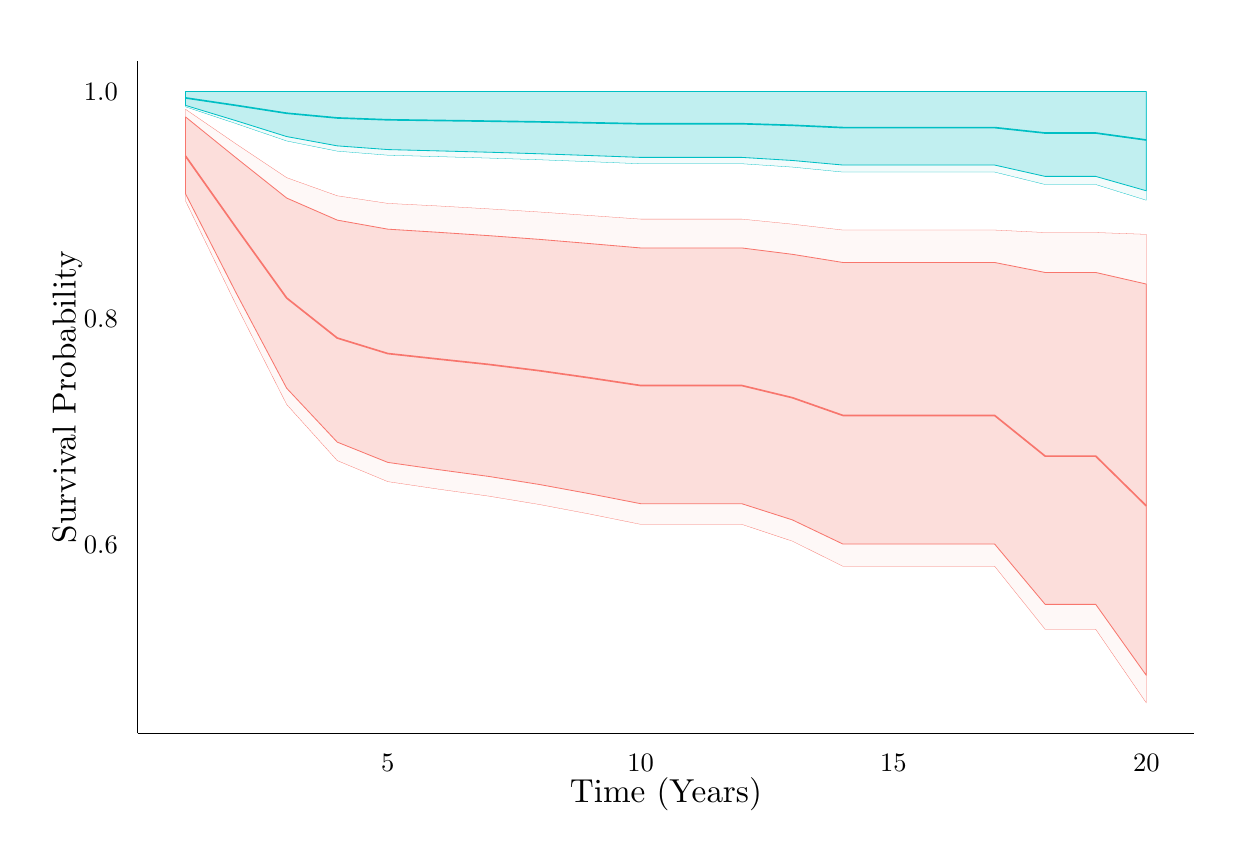
\begin{tikzpicture}[x=1pt,y=1pt]
\definecolor{fillColor}{RGB}{255,255,255}
\path[use as bounding box,fill=fillColor,fill opacity=0.00] (0,0) rectangle (433.62,289.08);
\begin{scope}
\path[clip] (  0.00,  0.00) rectangle (433.62,289.08);
\definecolor{drawColor}{RGB}{255,255,255}
\definecolor{fillColor}{RGB}{255,255,255}

\path[draw=drawColor,line width= 0.6pt,line join=round,line cap=round,fill=fillColor] (  0.00,  0.00) rectangle (433.62,289.08);
\end{scope}
\begin{scope}
\path[clip] ( 39.69, 34.03) rectangle (421.57,277.03);
\definecolor{fillColor}{RGB}{255,255,255}

\path[fill=fillColor] ( 39.69, 34.03) rectangle (421.58,277.03);
\definecolor{drawColor}{RGB}{248,118,109}

\path[draw=drawColor,line width= 0.6pt,line join=round] ( 57.05,242.67) --
	( 75.32,216.81) --
	( 93.59,191.39) --
	(111.86,176.93) --
	(130.13,171.32) --
	(148.41,169.33) --
	(166.68,167.38) --
	(184.95,165.12) --
	(203.22,162.52) --
	(221.49,159.77) --
	(239.77,159.77) --
	(258.04,159.77) --
	(276.31,155.37) --
	(294.58,148.96) --
	(312.86,148.96) --
	(331.13,148.96) --
	(349.40,148.96) --
	(367.67,134.25) --
	(385.94,134.25) --
	(404.22,116.27);
\definecolor{drawColor}{RGB}{0,191,196}

\path[draw=drawColor,line width= 0.6pt,line join=round] ( 57.05,263.69) --
	( 75.32,260.99) --
	( 93.59,258.16) --
	(111.86,256.46) --
	(130.13,255.79) --
	(148.41,255.54) --
	(166.68,255.30) --
	(184.95,255.03) --
	(203.22,254.70) --
	(221.49,254.36) --
	(239.77,254.36) --
	(258.04,254.36) --
	(276.31,253.80) --
	(294.58,252.97) --
	(312.86,252.97) --
	(331.13,252.97) --
	(349.40,252.97) --
	(367.67,251.01) --
	(385.94,251.01) --
	(404.22,248.49);
\definecolor{drawColor}{RGB}{248,118,109}
\definecolor{fillColor}{RGB}{248,118,109}

\path[draw=drawColor,line width= 0.1pt,line join=round,line cap=round,fill=fillColor,fill opacity=0.05] ( 57.05,259.58) --
	( 75.32,247.06) --
	( 93.59,234.87) --
	(111.86,228.33) --
	(130.13,225.58) --
	(148.41,224.65) --
	(166.68,223.60) --
	(184.95,222.47) --
	(203.22,221.19) --
	(221.49,219.90) --
	(239.77,219.90) --
	(258.04,219.90) --
	(276.31,218.08) --
	(294.58,215.95) --
	(312.86,215.95) --
	(331.13,215.95) --
	(349.40,215.95) --
	(367.67,215.05) --
	(385.94,215.05) --
	(404.22,214.40) --
	(404.22, 45.08) --
	(385.94, 71.67) --
	(367.67, 71.67) --
	(349.40, 94.47) --
	(331.13, 94.47) --
	(312.86, 94.47) --
	(294.58, 94.47) --
	(276.31,103.54) --
	(258.04,109.61) --
	(239.77,109.61) --
	(221.49,109.61) --
	(203.22,113.30) --
	(184.95,116.77) --
	(166.68,119.79) --
	(148.41,122.33) --
	(130.13,125.04) --
	(111.86,132.64) --
	( 93.59,152.92) --
	( 75.32,188.90) --
	( 57.05,226.46) --
	cycle;
\definecolor{drawColor}{RGB}{0,191,196}
\definecolor{fillColor}{RGB}{0,191,196}

\path[draw=drawColor,line width= 0.1pt,line join=round,line cap=round,fill=fillColor,fill opacity=0.05] ( 57.05,265.99) --
	( 75.32,265.99) --
	( 93.59,265.99) --
	(111.86,265.99) --
	(130.13,265.99) --
	(148.41,265.99) --
	(166.68,265.99) --
	(184.95,265.99) --
	(203.22,265.99) --
	(221.49,265.99) --
	(239.77,265.99) --
	(258.04,265.99) --
	(276.31,265.99) --
	(294.58,265.99) --
	(312.86,265.99) --
	(331.13,265.99) --
	(349.40,265.99) --
	(367.67,265.99) --
	(385.94,265.99) --
	(404.22,265.99) --
	(404.22,226.72) --
	(385.94,232.40) --
	(367.67,232.40) --
	(349.40,236.90) --
	(331.13,236.90) --
	(312.86,236.90) --
	(294.58,236.90) --
	(276.31,238.70) --
	(258.04,239.91) --
	(239.77,239.91) --
	(221.49,239.91) --
	(203.22,240.65) --
	(184.95,241.35) --
	(166.68,241.95) --
	(148.41,242.48) --
	(130.13,243.00) --
	(111.86,244.46) --
	( 93.59,248.14) --
	( 75.32,254.40) --
	( 57.05,260.47) --
	cycle;
\definecolor{drawColor}{RGB}{248,118,109}
\definecolor{fillColor}{RGB}{248,118,109}

\path[draw=drawColor,line width= 0.3pt,line join=round,line cap=round,fill=fillColor,fill opacity=0.20] ( 57.05,256.82) --
	( 75.32,242.03) --
	( 93.59,227.51) --
	(111.86,219.54) --
	(130.13,216.27) --
	(148.41,215.13) --
	(166.68,213.92) --
	(184.95,212.58) --
	(203.22,211.05) --
	(221.49,209.48) --
	(239.77,209.48) --
	(258.04,209.48) --
	(276.31,207.18) --
	(294.58,204.23) --
	(312.86,204.23) --
	(331.13,204.23) --
	(349.40,204.23) --
	(367.67,200.62) --
	(385.94,200.62) --
	(404.22,196.43) --
	(404.22, 55.04) --
	(385.94, 80.69) --
	(367.67, 80.69) --
	(349.40,102.49) --
	(331.13,102.49) --
	(312.86,102.49) --
	(294.58,102.49) --
	(276.31,111.22) --
	(258.04,117.07) --
	(239.77,117.07) --
	(221.49,117.07) --
	(203.22,120.64) --
	(184.95,124.00) --
	(166.68,126.91) --
	(148.41,129.38) --
	(130.13,131.99) --
	(111.86,139.32) --
	( 93.59,158.79) --
	( 75.32,193.24) --
	( 57.05,229.02) --
	cycle;
\definecolor{drawColor}{RGB}{0,191,196}
\definecolor{fillColor}{RGB}{0,191,196}

\path[draw=drawColor,line width= 0.3pt,line join=round,line cap=round,fill=fillColor,fill opacity=0.20] ( 57.05,265.99) --
	( 75.32,265.99) --
	( 93.59,265.99) --
	(111.86,265.99) --
	(130.13,265.99) --
	(148.41,265.99) --
	(166.68,265.99) --
	(184.95,265.99) --
	(203.22,265.99) --
	(221.49,265.99) --
	(239.77,265.99) --
	(258.04,265.99) --
	(276.31,265.99) --
	(294.58,265.99) --
	(312.86,265.99) --
	(331.13,265.99) --
	(349.40,265.99) --
	(367.67,265.99) --
	(385.94,265.99) --
	(404.22,265.99) --
	(404.22,230.14) --
	(385.94,235.33) --
	(367.67,235.33) --
	(349.40,239.44) --
	(331.13,239.44) --
	(312.86,239.44) --
	(294.58,239.44) --
	(276.31,241.09) --
	(258.04,242.20) --
	(239.77,242.20) --
	(221.49,242.20) --
	(203.22,242.87) --
	(184.95,243.51) --
	(166.68,244.07) --
	(148.41,244.55) --
	(130.13,245.03) --
	(111.86,246.37) --
	( 93.59,249.73) --
	( 75.32,255.45) --
	( 57.05,260.99) --
	cycle;
\end{scope}
\begin{scope}
\path[clip] (  0.00,  0.00) rectangle (433.62,289.08);
\definecolor{drawColor}{RGB}{0,0,0}

\path[draw=drawColor,line width= 0.6pt,line join=round] ( 39.69, 34.03) --
	( 39.69,277.03);
\end{scope}
\begin{scope}
\path[clip] (  0.00,  0.00) rectangle (433.62,289.08);
\definecolor{drawColor}{RGB}{0,0,0}

\node[text=drawColor,anchor=base east,inner sep=0pt, outer sep=0pt, scale=  0.96] at ( 32.57, 99.05) {0.6};

\node[text=drawColor,anchor=base east,inner sep=0pt, outer sep=0pt, scale=  0.96] at ( 32.57,180.86) {0.8};

\node[text=drawColor,anchor=base east,inner sep=0pt, outer sep=0pt, scale=  0.96] at ( 32.57,262.68) {1.0};
\end{scope}
\begin{scope}
\path[clip] (  0.00,  0.00) rectangle (433.62,289.08);
\definecolor{drawColor}{RGB}{0,0,0}

\path[draw=drawColor,line width= 0.6pt,line join=round] ( 39.69, 34.03) --
	(421.57, 34.03);
\end{scope}
\begin{scope}
\path[clip] (  0.00,  0.00) rectangle (433.62,289.08);
\definecolor{drawColor}{RGB}{0,0,0}

\node[text=drawColor,anchor=base,inner sep=0pt, outer sep=0pt, scale=  0.96] at (130.13, 20.31) {5};

\node[text=drawColor,anchor=base,inner sep=0pt, outer sep=0pt, scale=  0.96] at (221.49, 20.31) {10};

\node[text=drawColor,anchor=base,inner sep=0pt, outer sep=0pt, scale=  0.96] at (312.86, 20.31) {15};

\node[text=drawColor,anchor=base,inner sep=0pt, outer sep=0pt, scale=  0.96] at (404.22, 20.31) {20};
\end{scope}
\begin{scope}
\path[clip] (  0.00,  0.00) rectangle (433.62,289.08);
\definecolor{drawColor}{RGB}{0,0,0}

\node[text=drawColor,anchor=base,inner sep=0pt, outer sep=0pt, scale=  1.20] at (230.63,  9.03) {Time (Years)};
\end{scope}
\begin{scope}
\path[clip] (  0.00,  0.00) rectangle (433.62,289.08);
\definecolor{drawColor}{RGB}{0,0,0}

\node[text=drawColor,rotate= 90.00,anchor=base,inner sep=0pt, outer sep=0pt, scale=  1.20] at ( 17.30,155.53) {Survival Probability};
\end{scope}
\end{tikzpicture}
}
		\label{fig:compSancSurv}}	

	\end{tabular}

	\label{fig:surv3}	
\end{figure}


Our sanction reciprocity measure tells a similar story, but focuses on the consequences of past reciprocal adverse relations. Here we can see that countries whom have sanctioned each other in the past without complying to one another are not likely to comply to one another in the present. On the right side of Figure~\ref{fig:surv3}, we can again see that within just five years the probability of non-compliance in a case where target and sender states have not had adverse past relations is half compared to a case where past adverse relations are present. This points to important consequences for sender states, namely that continuous sanctioning of a particular state without that target every complying  may build up a resistance to compliance to future sanctions. 

\subsection*{Performance}

To assess the accuracy and performance of these estimates we employ a six-fold cross validation procedure.\footnote{Results of analysis were similar when employing a 10-fold cross validation as well, however, we limit to showing six here for the sake of space.} We use this procedure both to determine the robustness of our coefficient estimates when estimated on different subsamples of our dataset, and to assess how well the results of our model would generalize to an independent dataset. To begin the cross-validation, we split the 653 sanction cases in our dataset into six approximately equal subsets. We then run each model shown in Table~\ref{tab:regResults} six times, where in each iteration we left out one subsample to use as a test set. This allows us to compare the prediction accuracy of each model, thereby helping us to determine the gains from incorporating the reciprocity covariates that are key to our argument.

First, however, we show the results for our reciprocity covariates when we rerun our survival analysis on each of the six folds from the cross-validation. This analysis helps us to understand whether some of the subsets in our dataset follow a different pattern than what is in the broader set.\footnote{\cite{beck2008time}} Figure~\ref{fig:crossval} shows that this is not the case for the analysis we present here, the coefficient estimates for compliance and sanction reciprocity remain consistent across each of these subsamples.\footnote{The parameter estimates for the other covariates also remain consistent across each of the six folds but we leave them out here due to space constraints.}


\begin{figure}[ht]
	\centering
	\caption{Reciprocity coefficient estimates from each of the six-folds of the cross validation procedure.}
	\resizebox{1\textwidth}{!}{% Created by tikzDevice version 0.7.0 on 2014-08-02 16:07:02
% !TEX encoding = UTF-8 Unicode
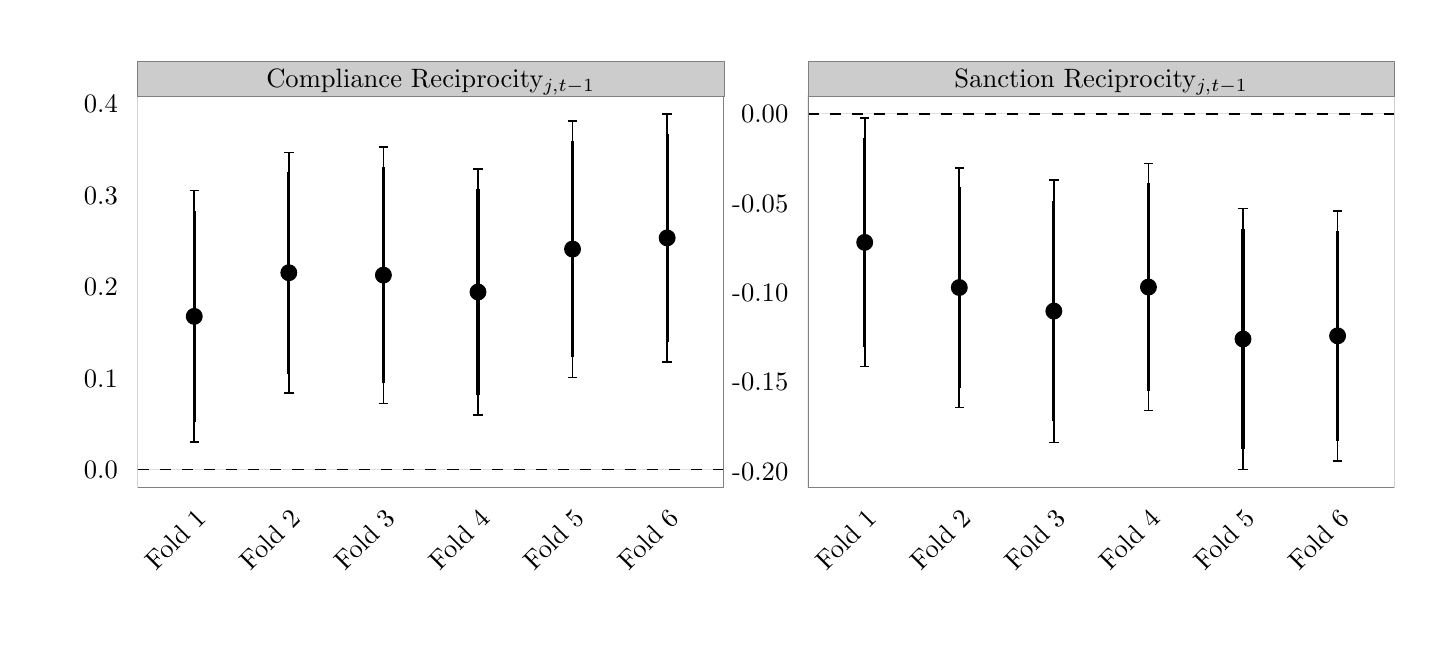
\begin{tikzpicture}[x=1pt,y=1pt]
\definecolor[named]{fillColor}{rgb}{1.00,1.00,1.00}
\path[use as bounding box,fill=fillColor,fill opacity=0.00] (0,0) rectangle (505.89,216.81);
\begin{scope}
\path[clip] (  0.00,  0.00) rectangle (505.89,216.81);
\definecolor[named]{drawColor}{rgb}{1.00,1.00,1.00}
\definecolor[named]{fillColor}{rgb}{1.00,1.00,1.00}

\path[draw=drawColor,line width= 0.6pt,line join=round,line cap=round,fill=fillColor] (  0.00,  0.00) rectangle (505.89,216.81);
\end{scope}
\begin{scope}
\path[clip] ( 39.69, 50.67) rectangle (251.57,192.13);
\definecolor[named]{fillColor}{rgb}{1.00,1.00,1.00}

\path[fill=fillColor] ( 39.69, 50.67) rectangle (251.57,192.13);
\definecolor[named]{drawColor}{rgb}{0.00,0.00,0.00}
\definecolor[named]{fillColor}{rgb}{0.00,0.00,0.00}

\path[draw=drawColor,draw opacity=0.30,line width= 0.3pt,line join=round,fill=fillColor,fill opacity=0.30] ( 60.19, 67.01) -- ( 60.19,157.97);

\path[draw=drawColor,draw opacity=0.30,line width= 0.3pt,line join=round,fill=fillColor,fill opacity=0.30] ( 94.37, 84.84) -- ( 94.37,171.68);

\path[draw=drawColor,draw opacity=0.30,line width= 0.3pt,line join=round,fill=fillColor,fill opacity=0.30] (128.54, 81.00) -- (128.54,173.77);

\path[draw=drawColor,draw opacity=0.30,line width= 0.3pt,line join=round,fill=fillColor,fill opacity=0.30] (162.72, 76.75) -- (162.72,165.85);

\path[draw=drawColor,draw opacity=0.30,line width= 0.3pt,line join=round,fill=fillColor,fill opacity=0.30] (196.89, 90.43) -- (196.89,183.18);

\path[draw=drawColor,draw opacity=0.30,line width= 0.3pt,line join=round,fill=fillColor,fill opacity=0.30] (231.07, 95.99) -- (231.07,185.70);
\definecolor[named]{drawColor}{rgb}{0.00,0.00,0.00}
\definecolor[named]{fillColor}{rgb}{0.00,0.00,0.00}

\path[draw=drawColor,line width= 1.1pt,line join=round,fill=fillColor] ( 60.19, 74.32) -- ( 60.19,150.66);

\path[draw=drawColor,line width= 1.1pt,line join=round,fill=fillColor] ( 94.37, 91.82) -- ( 94.37,164.70);

\path[draw=drawColor,line width= 1.1pt,line join=round,fill=fillColor] (128.54, 88.46) -- (128.54,166.31);

\path[draw=drawColor,line width= 1.1pt,line join=round,fill=fillColor] (162.72, 83.91) -- (162.72,158.69);

\path[draw=drawColor,line width= 1.1pt,line join=round,fill=fillColor] (196.89, 97.88) -- (196.89,175.73);

\path[draw=drawColor,line width= 1.1pt,line join=round,fill=fillColor] (231.07,103.20) -- (231.07,178.49);

\path[draw=drawColor,line width= 0.6pt,dash pattern=on 4pt off 4pt ,line join=round,fill=fillColor] ( 39.69, 57.10) -- (251.57, 57.10);

\path[draw=drawColor,line width= 0.4pt,line join=round,line cap=round,fill=fillColor] ( 60.19,112.49) circle (  2.85);

\path[draw=drawColor,line width= 0.4pt,line join=round,line cap=round,fill=fillColor] ( 94.37,128.26) circle (  2.85);

\path[draw=drawColor,line width= 0.4pt,line join=round,line cap=round,fill=fillColor] (128.54,127.39) circle (  2.85);

\path[draw=drawColor,line width= 0.4pt,line join=round,line cap=round,fill=fillColor] (162.72,121.30) circle (  2.85);

\path[draw=drawColor,line width= 0.4pt,line join=round,line cap=round,fill=fillColor] (196.89,136.80) circle (  2.85);

\path[draw=drawColor,line width= 0.4pt,line join=round,line cap=round,fill=fillColor] (231.07,140.84) circle (  2.85);

\path[draw=drawColor,line width= 0.6pt,line join=round] ( 58.48,157.97) --
	( 61.90,157.97);

\path[draw=drawColor,line width= 0.6pt,line join=round] ( 60.19,157.97) --
	( 60.19, 67.01);

\path[draw=drawColor,line width= 0.6pt,line join=round] ( 58.48, 67.01) --
	( 61.90, 67.01);

\path[draw=drawColor,line width= 0.6pt,line join=round] ( 92.66,171.68) --
	( 96.08,171.68);

\path[draw=drawColor,line width= 0.6pt,line join=round] ( 94.37,171.68) --
	( 94.37, 84.84);

\path[draw=drawColor,line width= 0.6pt,line join=round] ( 92.66, 84.84) --
	( 96.08, 84.84);

\path[draw=drawColor,line width= 0.6pt,line join=round] (126.83,173.77) --
	(130.25,173.77);

\path[draw=drawColor,line width= 0.6pt,line join=round] (128.54,173.77) --
	(128.54, 81.00);

\path[draw=drawColor,line width= 0.6pt,line join=round] (126.83, 81.00) --
	(130.25, 81.00);

\path[draw=drawColor,line width= 0.6pt,line join=round] (161.01,165.85) --
	(164.43,165.85);

\path[draw=drawColor,line width= 0.6pt,line join=round] (162.72,165.85) --
	(162.72, 76.75);

\path[draw=drawColor,line width= 0.6pt,line join=round] (161.01, 76.75) --
	(164.43, 76.75);

\path[draw=drawColor,line width= 0.6pt,line join=round] (195.18,183.18) --
	(198.60,183.18);

\path[draw=drawColor,line width= 0.6pt,line join=round] (196.89,183.18) --
	(196.89, 90.43);

\path[draw=drawColor,line width= 0.6pt,line join=round] (195.18, 90.43) --
	(198.60, 90.43);

\path[draw=drawColor,line width= 0.6pt,line join=round] (229.36,185.70) --
	(232.78,185.70);

\path[draw=drawColor,line width= 0.6pt,line join=round] (231.07,185.70) --
	(231.07, 95.99);

\path[draw=drawColor,line width= 0.6pt,line join=round] (229.36, 95.99) --
	(232.78, 95.99);
\definecolor[named]{drawColor}{rgb}{0.50,0.50,0.50}

\path[draw=drawColor,line width= 0.6pt,line join=round,line cap=round] ( 39.69, 50.67) rectangle (251.57,192.13);
\end{scope}
\begin{scope}
\path[clip] (281.96, 50.67) rectangle (493.85,192.13);
\definecolor[named]{fillColor}{rgb}{1.00,1.00,1.00}

\path[fill=fillColor] (281.96, 50.67) rectangle (493.85,192.13);
\definecolor[named]{drawColor}{rgb}{0.00,0.00,0.00}
\definecolor[named]{fillColor}{rgb}{0.00,0.00,0.00}

\path[draw=drawColor,draw opacity=0.30,line width= 0.3pt,line join=round,fill=fillColor,fill opacity=0.30] (302.46, 94.34) -- (302.46,184.13);

\path[draw=drawColor,draw opacity=0.30,line width= 0.3pt,line join=round,fill=fillColor,fill opacity=0.30] (336.64, 79.61) -- (336.64,166.21);

\path[draw=drawColor,draw opacity=0.30,line width= 0.3pt,line join=round,fill=fillColor,fill opacity=0.30] (370.81, 66.95) -- (370.81,161.82);

\path[draw=drawColor,draw opacity=0.30,line width= 0.3pt,line join=round,fill=fillColor,fill opacity=0.30] (404.99, 78.48) -- (404.99,167.69);

\path[draw=drawColor,draw opacity=0.30,line width= 0.3pt,line join=round,fill=fillColor,fill opacity=0.30] (439.16, 57.10) -- (439.16,151.50);

\path[draw=drawColor,draw opacity=0.30,line width= 0.3pt,line join=round,fill=fillColor,fill opacity=0.30] (473.34, 60.25) -- (473.34,150.65);
\definecolor[named]{drawColor}{rgb}{0.00,0.00,0.00}
\definecolor[named]{fillColor}{rgb}{0.00,0.00,0.00}

\path[draw=drawColor,line width= 1.1pt,line join=round,fill=fillColor] (302.46,101.55) -- (302.46,176.91);

\path[draw=drawColor,line width= 1.1pt,line join=round,fill=fillColor] (336.64, 86.57) -- (336.64,159.25);

\path[draw=drawColor,line width= 1.1pt,line join=round,fill=fillColor] (370.81, 74.58) -- (370.81,154.20);

\path[draw=drawColor,line width= 1.1pt,line join=round,fill=fillColor] (404.99, 85.65) -- (404.99,160.52);

\path[draw=drawColor,line width= 1.1pt,line join=round,fill=fillColor] (439.16, 64.69) -- (439.16,143.91);

\path[draw=drawColor,line width= 1.1pt,line join=round,fill=fillColor] (473.34, 67.52) -- (473.34,143.38);

\path[draw=drawColor,line width= 0.6pt,dash pattern=on 4pt off 4pt ,line join=round,fill=fillColor] (281.96,185.70) -- (493.85,185.70);

\path[draw=drawColor,line width= 0.4pt,line join=round,line cap=round,fill=fillColor] (302.46,139.23) circle (  2.85);

\path[draw=drawColor,line width= 0.4pt,line join=round,line cap=round,fill=fillColor] (336.64,122.91) circle (  2.85);

\path[draw=drawColor,line width= 0.4pt,line join=round,line cap=round,fill=fillColor] (370.81,114.39) circle (  2.85);

\path[draw=drawColor,line width= 0.4pt,line join=round,line cap=round,fill=fillColor] (404.99,123.08) circle (  2.85);

\path[draw=drawColor,line width= 0.4pt,line join=round,line cap=round,fill=fillColor] (439.16,104.30) circle (  2.85);

\path[draw=drawColor,line width= 0.4pt,line join=round,line cap=round,fill=fillColor] (473.34,105.45) circle (  2.85);

\path[draw=drawColor,line width= 0.6pt,line join=round] (300.76,184.13) --
	(304.17,184.13);

\path[draw=drawColor,line width= 0.6pt,line join=round] (302.46,184.13) --
	(302.46, 94.34);

\path[draw=drawColor,line width= 0.6pt,line join=round] (300.76, 94.34) --
	(304.17, 94.34);

\path[draw=drawColor,line width= 0.6pt,line join=round] (334.93,166.21) --
	(338.35,166.21);

\path[draw=drawColor,line width= 0.6pt,line join=round] (336.64,166.21) --
	(336.64, 79.61);

\path[draw=drawColor,line width= 0.6pt,line join=round] (334.93, 79.61) --
	(338.35, 79.61);

\path[draw=drawColor,line width= 0.6pt,line join=round] (369.11,161.82) --
	(372.52,161.82);

\path[draw=drawColor,line width= 0.6pt,line join=round] (370.81,161.82) --
	(370.81, 66.95);

\path[draw=drawColor,line width= 0.6pt,line join=round] (369.11, 66.95) --
	(372.52, 66.95);

\path[draw=drawColor,line width= 0.6pt,line join=round] (403.28,167.69) --
	(406.70,167.69);

\path[draw=drawColor,line width= 0.6pt,line join=round] (404.99,167.69) --
	(404.99, 78.48);

\path[draw=drawColor,line width= 0.6pt,line join=round] (403.28, 78.48) --
	(406.70, 78.48);

\path[draw=drawColor,line width= 0.6pt,line join=round] (437.46,151.50) --
	(440.87,151.50);

\path[draw=drawColor,line width= 0.6pt,line join=round] (439.16,151.50) --
	(439.16, 57.10);

\path[draw=drawColor,line width= 0.6pt,line join=round] (437.46, 57.10) --
	(440.87, 57.10);

\path[draw=drawColor,line width= 0.6pt,line join=round] (471.63,150.65) --
	(475.05,150.65);

\path[draw=drawColor,line width= 0.6pt,line join=round] (473.34,150.65) --
	(473.34, 60.25);

\path[draw=drawColor,line width= 0.6pt,line join=round] (471.63, 60.25) --
	(475.05, 60.25);
\definecolor[named]{drawColor}{rgb}{0.50,0.50,0.50}

\path[draw=drawColor,line width= 0.6pt,line join=round,line cap=round] (281.96, 50.67) rectangle (493.85,192.13);
\end{scope}
\begin{scope}
\path[clip] (  0.00,  0.00) rectangle (505.89,216.81);
\definecolor[named]{drawColor}{rgb}{0.50,0.50,0.50}
\definecolor[named]{fillColor}{rgb}{0.80,0.80,0.80}

\path[draw=drawColor,line width= 0.2pt,line join=round,line cap=round,fill=fillColor] ( 39.69,192.13) rectangle (251.57,204.77);
\definecolor[named]{drawColor}{rgb}{0.00,0.00,0.00}

\node[text=drawColor,anchor=base,inner sep=0pt, outer sep=0pt, scale=  0.96] at (145.63,195.14) {Compliance Reciprocity$_{j,t-1}$};
\end{scope}
\begin{scope}
\path[clip] (  0.00,  0.00) rectangle (505.89,216.81);
\definecolor[named]{drawColor}{rgb}{0.50,0.50,0.50}
\definecolor[named]{fillColor}{rgb}{0.80,0.80,0.80}

\path[draw=drawColor,line width= 0.2pt,line join=round,line cap=round,fill=fillColor] (281.96,192.13) rectangle (493.85,204.77);
\definecolor[named]{drawColor}{rgb}{0.00,0.00,0.00}

\node[text=drawColor,anchor=base,inner sep=0pt, outer sep=0pt, scale=  0.96] at (387.90,195.14) {Sanction Reciprocity$_{j,t-1}$};
\end{scope}
\begin{scope}
\path[clip] (  0.00,  0.00) rectangle (505.89,216.81);
\definecolor[named]{drawColor}{rgb}{0.00,0.00,0.00}

\node[text=drawColor,anchor=base east,inner sep=0pt, outer sep=0pt, scale=  0.96] at ( 32.57, 53.79) {0.0};

\node[text=drawColor,anchor=base east,inner sep=0pt, outer sep=0pt, scale=  0.96] at ( 32.57, 86.88) {0.1};

\node[text=drawColor,anchor=base east,inner sep=0pt, outer sep=0pt, scale=  0.96] at ( 32.57,119.97) {0.2};

\node[text=drawColor,anchor=base east,inner sep=0pt, outer sep=0pt, scale=  0.96] at ( 32.57,153.05) {0.3};

\node[text=drawColor,anchor=base east,inner sep=0pt, outer sep=0pt, scale=  0.96] at ( 32.57,186.14) {0.4};
\end{scope}
\begin{scope}
\path[clip] (  0.00,  0.00) rectangle (505.89,216.81);
\definecolor[named]{drawColor}{rgb}{0.00,0.00,0.00}

\node[text=drawColor,anchor=base east,inner sep=0pt, outer sep=0pt, scale=  0.96] at (274.85, 53.29) {-0.20};

\node[text=drawColor,anchor=base east,inner sep=0pt, outer sep=0pt, scale=  0.96] at (274.85, 85.57) {-0.15};

\node[text=drawColor,anchor=base east,inner sep=0pt, outer sep=0pt, scale=  0.96] at (274.85,117.84) {-0.10};

\node[text=drawColor,anchor=base east,inner sep=0pt, outer sep=0pt, scale=  0.96] at (274.85,150.12) {-0.05};

\node[text=drawColor,anchor=base east,inner sep=0pt, outer sep=0pt, scale=  0.96] at (274.85,182.39) {0.00};
\end{scope}
\begin{scope}
\path[clip] (  0.00,  0.00) rectangle (505.89,216.81);
\definecolor[named]{drawColor}{rgb}{0.00,0.00,0.00}

\node[text=drawColor,rotate= 45.00,anchor=base east,inner sep=0pt, outer sep=0pt, scale=  0.96] at ( 64.87, 38.88) {Fold 1};

\node[text=drawColor,rotate= 45.00,anchor=base east,inner sep=0pt, outer sep=0pt, scale=  0.96] at ( 99.04, 38.88) {Fold 2};

\node[text=drawColor,rotate= 45.00,anchor=base east,inner sep=0pt, outer sep=0pt, scale=  0.96] at (133.22, 38.88) {Fold 3};

\node[text=drawColor,rotate= 45.00,anchor=base east,inner sep=0pt, outer sep=0pt, scale=  0.96] at (167.39, 38.88) {Fold 4};

\node[text=drawColor,rotate= 45.00,anchor=base east,inner sep=0pt, outer sep=0pt, scale=  0.96] at (201.57, 38.88) {Fold 5};

\node[text=drawColor,rotate= 45.00,anchor=base east,inner sep=0pt, outer sep=0pt, scale=  0.96] at (235.74, 38.88) {Fold 6};
\end{scope}
\begin{scope}
\path[clip] (  0.00,  0.00) rectangle (505.89,216.81);
\definecolor[named]{drawColor}{rgb}{0.00,0.00,0.00}

\node[text=drawColor,rotate= 45.00,anchor=base east,inner sep=0pt, outer sep=0pt, scale=  0.96] at (307.14, 38.88) {Fold 1};

\node[text=drawColor,rotate= 45.00,anchor=base east,inner sep=0pt, outer sep=0pt, scale=  0.96] at (341.31, 38.88) {Fold 2};

\node[text=drawColor,rotate= 45.00,anchor=base east,inner sep=0pt, outer sep=0pt, scale=  0.96] at (375.49, 38.88) {Fold 3};

\node[text=drawColor,rotate= 45.00,anchor=base east,inner sep=0pt, outer sep=0pt, scale=  0.96] at (409.66, 38.88) {Fold 4};

\node[text=drawColor,rotate= 45.00,anchor=base east,inner sep=0pt, outer sep=0pt, scale=  0.96] at (443.84, 38.88) {Fold 5};

\node[text=drawColor,rotate= 45.00,anchor=base east,inner sep=0pt, outer sep=0pt, scale=  0.96] at (478.02, 38.88) {Fold 6};
\end{scope}
\end{tikzpicture}
}
	\label{fig:crossval}
\end{figure}


A key question that remains, however, is whether we are able to better explain sanction compliance through the incorporation of these network level covariates. Figure~\ref{fig:auc} shows out-of-sample time-dependent AUC results from the six-fold cross validation procedure. When calculating the time-dependent AUC we vary the time parameter to range from 0 to 15 years.\footnote{Time-dependent AUCs were computed using the formula provided by \citet{chambless2006estimation}.} We set the max for 15 years because only 4\% of sanction cases in our dataset that extend past 15 years end with compliance by a target state. This leads to the AUC statistics for each model. After that time point, the accuracy of any of the models begin to coalesce. Before the 15 year mark, however, we see noticeable variation in the time-dependent AUC statistics for each model. Most importantly, we can see that Model 3, where we incorporate our network level covariates, provides a noticeably higher AUC than the alternatives that we examined. Even simply accounting for proximate relationships, as we did in Model 2, does not provide a noticeably higher level of performance than target-state focused explanations.

\begin{figure}[ht]
	\centering
	\caption{Out-of-sample time-dependent AUC statistics from six-fold cross validation procedure for each model shown in Table~\ref{tab:regResults}. The solid line represents Model 1, the dotted line represents Model2, and the dashed line represents Model 3.}
	\resizebox{0.8\textwidth}{!}{% Created by tikzDevice version 0.6.1 on 2016-06-13 09:53:06
% !TEX encoding = UTF-8 Unicode
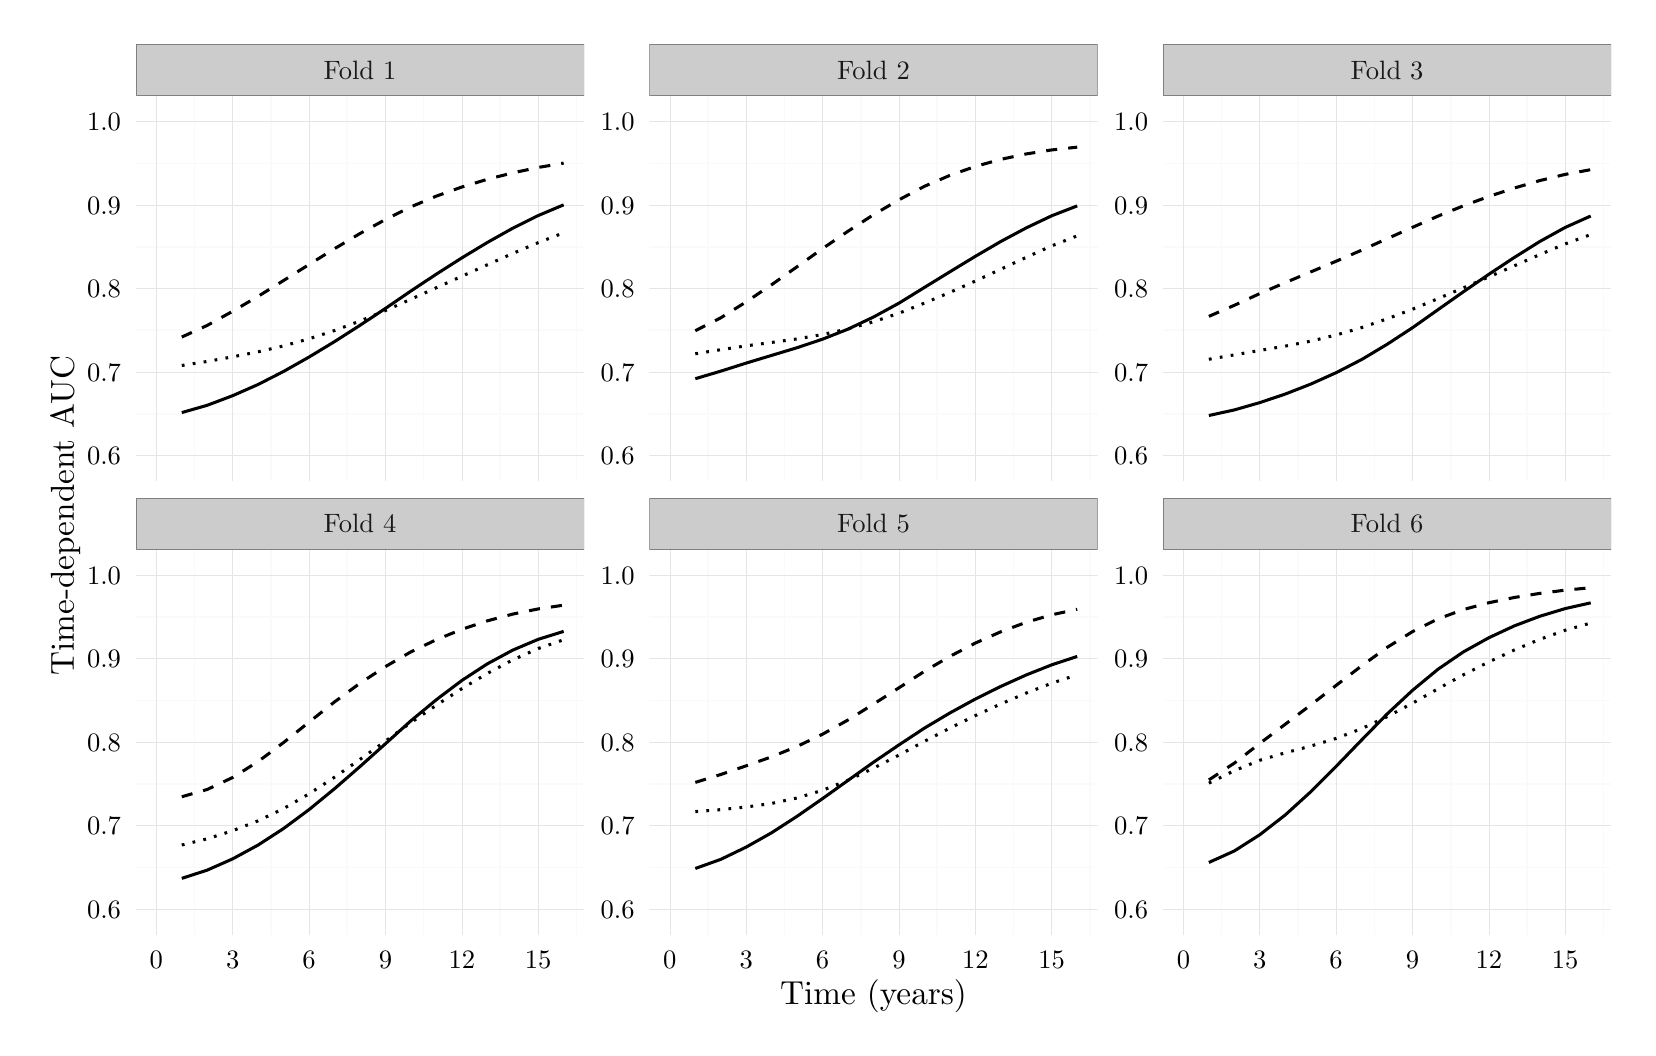
\begin{tikzpicture}[x=1pt,y=1pt]
\definecolor[named]{drawColor}{rgb}{0.00,0.00,0.00}
\definecolor[named]{fillColor}{rgb}{1.00,1.00,1.00}
\fill[color=fillColor,] (0,0) rectangle (578.16,361.35);
\begin{scope}
\path[clip] (  0.00,  0.00) rectangle (578.16,361.35);
\end{scope}
\begin{scope}
\path[clip] (  0.00,  0.00) rectangle (578.16,361.35);
\end{scope}
\begin{scope}
\path[clip] (  0.00,  0.00) rectangle (578.16,361.35);
\end{scope}
\begin{scope}
\path[clip] (  0.00,  0.00) rectangle (578.16,361.35);
\end{scope}
\begin{scope}
\path[clip] (  0.00,  0.00) rectangle (578.16,361.35);
\end{scope}
\begin{scope}
\path[clip] (  0.00,  0.00) rectangle (578.16,361.35);
\end{scope}
\begin{scope}
\path[clip] (  0.00,  0.00) rectangle (578.16,361.35);
\end{scope}
\begin{scope}
\path[clip] (  0.00,  0.00) rectangle (578.16,361.35);
\end{scope}
\begin{scope}
\path[clip] (  0.00,  0.00) rectangle (578.16,361.35);
\end{scope}
\begin{scope}
\path[clip] (  0.00,  0.00) rectangle (578.16,361.35);
\end{scope}
\begin{scope}
\path[clip] (  0.00,  0.00) rectangle (578.16,361.35);
\end{scope}
\begin{scope}
\path[clip] (  0.00,  0.00) rectangle (578.16,361.35);
\end{scope}
\begin{scope}
\path[clip] (  0.00,  0.00) rectangle (578.16,361.35);
\end{scope}
\begin{scope}
\path[clip] (  0.00,  0.00) rectangle (578.16,361.35);
\end{scope}
\begin{scope}
\path[clip] (  0.00,  0.00) rectangle (578.16,361.35);
\end{scope}
\begin{scope}
\path[clip] (  0.00,  0.00) rectangle (578.16,361.35);
\end{scope}
\begin{scope}
\path[clip] (  0.00,  0.00) rectangle (578.16,361.35);
\end{scope}
\begin{scope}
\path[clip] (  0.00,  0.00) rectangle (578.16,361.35);
\end{scope}
\begin{scope}
\path[clip] (  0.00,  0.00) rectangle (578.16,361.35);
\end{scope}
\begin{scope}
\path[clip] (  0.00,  0.00) rectangle (578.16,361.35);
\end{scope}
\begin{scope}
\path[clip] (  0.00,  0.00) rectangle (578.16,361.35);
\end{scope}
\begin{scope}
\path[clip] (  0.00,  0.00) rectangle (578.16,361.35);
\end{scope}
\begin{scope}
\path[clip] (  0.00,  0.00) rectangle (578.16,361.35);
\end{scope}
\begin{scope}
\path[clip] (  0.00,  0.00) rectangle (578.16,361.35);
\end{scope}
\begin{scope}
\path[clip] (  0.00,  0.00) rectangle (578.16,361.35);
\end{scope}
\begin{scope}
\path[clip] (  0.00,  0.00) rectangle (578.16,361.35);
\end{scope}
\begin{scope}
\path[clip] (  0.00,  0.00) rectangle (578.16,361.35);
\end{scope}
\begin{scope}
\path[clip] (  0.00,  0.00) rectangle (578.16,361.35);
\definecolor[named]{drawColor}{rgb}{1.00,1.00,1.00}
\definecolor[named]{fillColor}{rgb}{1.00,1.00,1.00}

\draw[color=drawColor,line width= 0.6pt,line cap=round,line join=round,fill=fillColor,] (  0.00,  0.00) rectangle (578.16,361.35);
\end{scope}
\begin{scope}
\path[clip] (  0.00,  0.00) rectangle (578.16,361.35);
\end{scope}
\begin{scope}
\path[clip] ( 39.13,197.41) rectangle (201.03,336.74);
\definecolor[named]{fillColor}{rgb}{1.00,1.00,1.00}

\draw[fill=fillColor,draw opacity=0.00,] ( 39.13,197.41) rectangle (201.03,336.74);
\definecolor[named]{drawColor}{rgb}{0.98,0.98,0.98}

\draw[color=drawColor,line width= 0.6pt,line join=round,fill opacity=0.00,] ( 39.13,221.84) --
	(201.03,221.84);

\draw[color=drawColor,line width= 0.6pt,line join=round,fill opacity=0.00,] ( 39.13,252.00) --
	(201.03,252.00);

\draw[color=drawColor,line width= 0.6pt,line join=round,fill opacity=0.00,] ( 39.13,282.15) --
	(201.03,282.15);

\draw[color=drawColor,line width= 0.6pt,line join=round,fill opacity=0.00,] ( 39.13,312.31) --
	(201.03,312.31);

\draw[color=drawColor,line width= 0.6pt,line join=round,fill opacity=0.00,] ( 60.29,197.41) --
	( 60.29,336.74);

\draw[color=drawColor,line width= 0.6pt,line join=round,fill opacity=0.00,] ( 87.88,197.41) --
	( 87.88,336.74);

\draw[color=drawColor,line width= 0.6pt,line join=round,fill opacity=0.00,] (115.48,197.41) --
	(115.48,336.74);

\draw[color=drawColor,line width= 0.6pt,line join=round,fill opacity=0.00,] (143.08,197.41) --
	(143.08,336.74);

\draw[color=drawColor,line width= 0.6pt,line join=round,fill opacity=0.00,] (170.67,197.41) --
	(170.67,336.74);

\draw[color=drawColor,line width= 0.6pt,line join=round,fill opacity=0.00,] (198.27,197.41) --
	(198.27,336.74);
\definecolor[named]{drawColor}{rgb}{0.90,0.90,0.90}

\draw[color=drawColor,line width= 0.2pt,line join=round,fill opacity=0.00,] ( 39.13,206.76) --
	(201.03,206.76);

\draw[color=drawColor,line width= 0.2pt,line join=round,fill opacity=0.00,] ( 39.13,236.92) --
	(201.03,236.92);

\draw[color=drawColor,line width= 0.2pt,line join=round,fill opacity=0.00,] ( 39.13,267.08) --
	(201.03,267.08);

\draw[color=drawColor,line width= 0.2pt,line join=round,fill opacity=0.00,] ( 39.13,297.23) --
	(201.03,297.23);

\draw[color=drawColor,line width= 0.2pt,line join=round,fill opacity=0.00,] ( 39.13,327.39) --
	(201.03,327.39);

\draw[color=drawColor,line width= 0.2pt,line join=round,fill opacity=0.00,] ( 46.49,197.41) --
	( 46.49,336.74);

\draw[color=drawColor,line width= 0.2pt,line join=round,fill opacity=0.00,] ( 74.08,197.41) --
	( 74.08,336.74);

\draw[color=drawColor,line width= 0.2pt,line join=round,fill opacity=0.00,] (101.68,197.41) --
	(101.68,336.74);

\draw[color=drawColor,line width= 0.2pt,line join=round,fill opacity=0.00,] (129.28,197.41) --
	(129.28,336.74);

\draw[color=drawColor,line width= 0.2pt,line join=round,fill opacity=0.00,] (156.87,197.41) --
	(156.87,336.74);

\draw[color=drawColor,line width= 0.2pt,line join=round,fill opacity=0.00,] (184.47,197.41) --
	(184.47,336.74);
\definecolor[named]{drawColor}{rgb}{0.00,0.00,0.00}
\definecolor[named]{fillColor}{rgb}{0.00,0.00,0.00}

\draw[color=drawColor,line width= 1.1pt,line join=round,] ( 55.69,222.26) --
	( 64.89,224.90) --
	( 74.08,228.37) --
	( 83.28,232.42) --
	( 92.48,237.13) --
	(101.68,242.33) --
	(110.88,247.90) --
	(120.08,253.79) --
	(129.28,259.90) --
	(138.48,266.20) --
	(147.68,272.29) --
	(156.87,278.15) --
	(166.07,283.71) --
	(175.27,288.87) --
	(184.47,293.45) --
	(193.67,297.33);

\draw[color=drawColor,line width= 1.1pt,dash pattern=on 1pt off 3pt ,line join=round,] ( 55.69,239.28) --
	( 64.89,240.74) --
	( 74.08,242.41) --
	( 83.28,244.22) --
	( 92.48,246.36) --
	(101.68,248.91) --
	(110.88,251.91) --
	(120.08,255.34) --
	(129.28,259.13) --
	(138.48,263.24) --
	(147.68,267.37) --
	(156.87,271.52) --
	(166.07,275.66) --
	(175.27,279.76) --
	(184.47,283.66) --
	(193.67,287.22);

\draw[color=drawColor,line width= 1.1pt,dash pattern=on 4pt off 4pt ,line join=round,] ( 55.69,249.56) --
	( 64.89,253.77) --
	( 74.08,258.88) --
	( 83.28,264.27) --
	( 92.48,269.99) --
	(101.68,275.77) --
	(110.88,281.48) --
	(120.08,286.96) --
	(129.28,292.02) --
	(138.48,296.61) --
	(147.68,300.48) --
	(156.87,303.76) --
	(166.07,306.54) --
	(175.27,308.88) --
	(184.47,310.83) --
	(193.67,312.40);
\end{scope}
\begin{scope}
\path[clip] (  0.00,  0.00) rectangle (578.16,361.35);
\end{scope}
\begin{scope}
\path[clip] (224.69,197.41) rectangle (386.59,336.74);
\definecolor[named]{fillColor}{rgb}{1.00,1.00,1.00}

\draw[fill=fillColor,draw opacity=0.00,] (224.69,197.41) rectangle (386.59,336.74);
\definecolor[named]{drawColor}{rgb}{0.98,0.98,0.98}

\draw[color=drawColor,line width= 0.6pt,line join=round,fill opacity=0.00,] (224.69,221.84) --
	(386.59,221.84);

\draw[color=drawColor,line width= 0.6pt,line join=round,fill opacity=0.00,] (224.69,252.00) --
	(386.59,252.00);

\draw[color=drawColor,line width= 0.6pt,line join=round,fill opacity=0.00,] (224.69,282.15) --
	(386.59,282.15);

\draw[color=drawColor,line width= 0.6pt,line join=round,fill opacity=0.00,] (224.69,312.31) --
	(386.59,312.31);

\draw[color=drawColor,line width= 0.6pt,line join=round,fill opacity=0.00,] (245.85,197.41) --
	(245.85,336.74);

\draw[color=drawColor,line width= 0.6pt,line join=round,fill opacity=0.00,] (273.45,197.41) --
	(273.45,336.74);

\draw[color=drawColor,line width= 0.6pt,line join=round,fill opacity=0.00,] (301.04,197.41) --
	(301.04,336.74);

\draw[color=drawColor,line width= 0.6pt,line join=round,fill opacity=0.00,] (328.64,197.41) --
	(328.64,336.74);

\draw[color=drawColor,line width= 0.6pt,line join=round,fill opacity=0.00,] (356.24,197.41) --
	(356.24,336.74);

\draw[color=drawColor,line width= 0.6pt,line join=round,fill opacity=0.00,] (383.84,197.41) --
	(383.84,336.74);
\definecolor[named]{drawColor}{rgb}{0.90,0.90,0.90}

\draw[color=drawColor,line width= 0.2pt,line join=round,fill opacity=0.00,] (224.69,206.76) --
	(386.59,206.76);

\draw[color=drawColor,line width= 0.2pt,line join=round,fill opacity=0.00,] (224.69,236.92) --
	(386.59,236.92);

\draw[color=drawColor,line width= 0.2pt,line join=round,fill opacity=0.00,] (224.69,267.08) --
	(386.59,267.08);

\draw[color=drawColor,line width= 0.2pt,line join=round,fill opacity=0.00,] (224.69,297.23) --
	(386.59,297.23);

\draw[color=drawColor,line width= 0.2pt,line join=round,fill opacity=0.00,] (224.69,327.39) --
	(386.59,327.39);

\draw[color=drawColor,line width= 0.2pt,line join=round,fill opacity=0.00,] (232.05,197.41) --
	(232.05,336.74);

\draw[color=drawColor,line width= 0.2pt,line join=round,fill opacity=0.00,] (259.65,197.41) --
	(259.65,336.74);

\draw[color=drawColor,line width= 0.2pt,line join=round,fill opacity=0.00,] (287.25,197.41) --
	(287.25,336.74);

\draw[color=drawColor,line width= 0.2pt,line join=round,fill opacity=0.00,] (314.84,197.41) --
	(314.84,336.74);

\draw[color=drawColor,line width= 0.2pt,line join=round,fill opacity=0.00,] (342.44,197.41) --
	(342.44,336.74);

\draw[color=drawColor,line width= 0.2pt,line join=round,fill opacity=0.00,] (370.04,197.41) --
	(370.04,336.74);
\definecolor[named]{drawColor}{rgb}{0.00,0.00,0.00}
\definecolor[named]{fillColor}{rgb}{0.00,0.00,0.00}

\draw[color=drawColor,line width= 1.1pt,line join=round,] (241.25,234.50) --
	(250.45,237.23) --
	(259.65,240.15) --
	(268.85,242.93) --
	(278.05,245.71) --
	(287.25,248.80) --
	(296.45,252.42) --
	(305.64,256.79) --
	(314.84,261.80) --
	(324.04,267.48) --
	(333.24,273.13) --
	(342.44,278.72) --
	(351.64,284.09) --
	(360.84,289.00) --
	(370.04,293.38) --
	(379.24,296.94);

\draw[color=drawColor,line width= 1.1pt,dash pattern=on 1pt off 3pt ,line join=round,] (241.25,243.51) --
	(250.45,244.98) --
	(259.65,246.38) --
	(268.85,247.61) --
	(278.05,248.89) --
	(287.25,250.47) --
	(296.45,252.50) --
	(305.64,255.08) --
	(314.84,258.17) --
	(324.04,261.82) --
	(333.24,265.68) --
	(342.44,269.79) --
	(351.64,274.07) --
	(360.84,278.36) --
	(370.04,282.51) --
	(379.24,286.11);

\draw[color=drawColor,line width= 1.1pt,dash pattern=on 4pt off 4pt ,line join=round,] (241.25,251.85) --
	(250.45,256.51) --
	(259.65,262.28) --
	(268.85,268.48) --
	(278.05,274.98) --
	(287.25,281.54) --
	(296.45,287.81) --
	(305.64,293.76) --
	(314.84,299.15) --
	(324.04,304.02) --
	(333.24,307.97) --
	(342.44,311.20) --
	(351.64,313.77) --
	(360.84,315.72) --
	(370.04,317.17) --
	(379.24,318.17);
\end{scope}
\begin{scope}
\path[clip] (  0.00,  0.00) rectangle (578.16,361.35);
\end{scope}
\begin{scope}
\path[clip] (410.26,197.41) rectangle (572.16,336.74);
\definecolor[named]{fillColor}{rgb}{1.00,1.00,1.00}

\draw[fill=fillColor,draw opacity=0.00,] (410.26,197.41) rectangle (572.16,336.74);
\definecolor[named]{drawColor}{rgb}{0.98,0.98,0.98}

\draw[color=drawColor,line width= 0.6pt,line join=round,fill opacity=0.00,] (410.26,221.84) --
	(572.16,221.84);

\draw[color=drawColor,line width= 0.6pt,line join=round,fill opacity=0.00,] (410.26,252.00) --
	(572.16,252.00);

\draw[color=drawColor,line width= 0.6pt,line join=round,fill opacity=0.00,] (410.26,282.15) --
	(572.16,282.15);

\draw[color=drawColor,line width= 0.6pt,line join=round,fill opacity=0.00,] (410.26,312.31) --
	(572.16,312.31);

\draw[color=drawColor,line width= 0.6pt,line join=round,fill opacity=0.00,] (431.42,197.41) --
	(431.42,336.74);

\draw[color=drawColor,line width= 0.6pt,line join=round,fill opacity=0.00,] (459.01,197.41) --
	(459.01,336.74);

\draw[color=drawColor,line width= 0.6pt,line join=round,fill opacity=0.00,] (486.61,197.41) --
	(486.61,336.74);

\draw[color=drawColor,line width= 0.6pt,line join=round,fill opacity=0.00,] (514.21,197.41) --
	(514.21,336.74);

\draw[color=drawColor,line width= 0.6pt,line join=round,fill opacity=0.00,] (541.80,197.41) --
	(541.80,336.74);

\draw[color=drawColor,line width= 0.6pt,line join=round,fill opacity=0.00,] (569.40,197.41) --
	(569.40,336.74);
\definecolor[named]{drawColor}{rgb}{0.90,0.90,0.90}

\draw[color=drawColor,line width= 0.2pt,line join=round,fill opacity=0.00,] (410.26,206.76) --
	(572.16,206.76);

\draw[color=drawColor,line width= 0.2pt,line join=round,fill opacity=0.00,] (410.26,236.92) --
	(572.16,236.92);

\draw[color=drawColor,line width= 0.2pt,line join=round,fill opacity=0.00,] (410.26,267.08) --
	(572.16,267.08);

\draw[color=drawColor,line width= 0.2pt,line join=round,fill opacity=0.00,] (410.26,297.23) --
	(572.16,297.23);

\draw[color=drawColor,line width= 0.2pt,line join=round,fill opacity=0.00,] (410.26,327.39) --
	(572.16,327.39);

\draw[color=drawColor,line width= 0.2pt,line join=round,fill opacity=0.00,] (417.62,197.41) --
	(417.62,336.74);

\draw[color=drawColor,line width= 0.2pt,line join=round,fill opacity=0.00,] (445.21,197.41) --
	(445.21,336.74);

\draw[color=drawColor,line width= 0.2pt,line join=round,fill opacity=0.00,] (472.81,197.41) --
	(472.81,336.74);

\draw[color=drawColor,line width= 0.2pt,line join=round,fill opacity=0.00,] (500.41,197.41) --
	(500.41,336.74);

\draw[color=drawColor,line width= 0.2pt,line join=round,fill opacity=0.00,] (528.01,197.41) --
	(528.01,336.74);

\draw[color=drawColor,line width= 0.2pt,line join=round,fill opacity=0.00,] (555.60,197.41) --
	(555.60,336.74);
\definecolor[named]{drawColor}{rgb}{0.00,0.00,0.00}
\definecolor[named]{fillColor}{rgb}{0.00,0.00,0.00}

\draw[color=drawColor,line width= 1.1pt,line join=round,] (426.82,221.20) --
	(436.02,223.22) --
	(445.21,225.86) --
	(454.41,228.95) --
	(463.61,232.54) --
	(472.81,236.68) --
	(482.01,241.42) --
	(491.21,246.92) --
	(500.41,252.93) --
	(509.61,259.44) --
	(518.81,265.92) --
	(528.01,272.24) --
	(537.20,278.32) --
	(546.40,284.08) --
	(555.60,289.17) --
	(564.80,293.29);

\draw[color=drawColor,line width= 1.1pt,dash pattern=on 1pt off 3pt ,line join=round,] (426.82,241.53) --
	(436.02,243.12) --
	(445.21,244.71) --
	(454.41,246.27) --
	(463.61,248.07) --
	(472.81,250.29) --
	(482.01,252.97) --
	(491.21,256.13) --
	(500.41,259.61) --
	(509.61,263.44) --
	(518.81,267.34) --
	(528.01,271.29) --
	(537.20,275.30) --
	(546.40,279.35) --
	(555.60,283.21) --
	(564.80,286.58);

\draw[color=drawColor,line width= 1.1pt,dash pattern=on 4pt off 4pt ,line join=round,] (426.82,257.03) --
	(436.02,261.02) --
	(445.21,265.26) --
	(454.41,269.21) --
	(463.61,273.08) --
	(472.81,276.95) --
	(482.01,280.94) --
	(491.21,285.09) --
	(500.41,289.19) --
	(509.61,293.25) --
	(518.81,296.98) --
	(528.01,300.36) --
	(537.20,303.40) --
	(546.40,306.09) --
	(555.60,308.33) --
	(564.80,310.04);
\end{scope}
\begin{scope}
\path[clip] (  0.00,  0.00) rectangle (578.16,361.35);
\end{scope}
\begin{scope}
\path[clip] ( 39.13, 33.48) rectangle (201.03,172.80);
\definecolor[named]{fillColor}{rgb}{1.00,1.00,1.00}

\draw[fill=fillColor,draw opacity=0.00,] ( 39.13, 33.48) rectangle (201.03,172.80);
\definecolor[named]{drawColor}{rgb}{0.98,0.98,0.98}

\draw[color=drawColor,line width= 0.6pt,line join=round,fill opacity=0.00,] ( 39.13, 57.90) --
	(201.03, 57.90);

\draw[color=drawColor,line width= 0.6pt,line join=round,fill opacity=0.00,] ( 39.13, 88.06) --
	(201.03, 88.06);

\draw[color=drawColor,line width= 0.6pt,line join=round,fill opacity=0.00,] ( 39.13,118.22) --
	(201.03,118.22);

\draw[color=drawColor,line width= 0.6pt,line join=round,fill opacity=0.00,] ( 39.13,148.37) --
	(201.03,148.37);

\draw[color=drawColor,line width= 0.6pt,line join=round,fill opacity=0.00,] ( 60.29, 33.48) --
	( 60.29,172.80);

\draw[color=drawColor,line width= 0.6pt,line join=round,fill opacity=0.00,] ( 87.88, 33.48) --
	( 87.88,172.80);

\draw[color=drawColor,line width= 0.6pt,line join=round,fill opacity=0.00,] (115.48, 33.48) --
	(115.48,172.80);

\draw[color=drawColor,line width= 0.6pt,line join=round,fill opacity=0.00,] (143.08, 33.48) --
	(143.08,172.80);

\draw[color=drawColor,line width= 0.6pt,line join=round,fill opacity=0.00,] (170.67, 33.48) --
	(170.67,172.80);

\draw[color=drawColor,line width= 0.6pt,line join=round,fill opacity=0.00,] (198.27, 33.48) --
	(198.27,172.80);
\definecolor[named]{drawColor}{rgb}{0.90,0.90,0.90}

\draw[color=drawColor,line width= 0.2pt,line join=round,fill opacity=0.00,] ( 39.13, 42.83) --
	(201.03, 42.83);

\draw[color=drawColor,line width= 0.2pt,line join=round,fill opacity=0.00,] ( 39.13, 72.98) --
	(201.03, 72.98);

\draw[color=drawColor,line width= 0.2pt,line join=round,fill opacity=0.00,] ( 39.13,103.14) --
	(201.03,103.14);

\draw[color=drawColor,line width= 0.2pt,line join=round,fill opacity=0.00,] ( 39.13,133.30) --
	(201.03,133.30);

\draw[color=drawColor,line width= 0.2pt,line join=round,fill opacity=0.00,] ( 39.13,163.45) --
	(201.03,163.45);

\draw[color=drawColor,line width= 0.2pt,line join=round,fill opacity=0.00,] ( 46.49, 33.48) --
	( 46.49,172.80);

\draw[color=drawColor,line width= 0.2pt,line join=round,fill opacity=0.00,] ( 74.08, 33.48) --
	( 74.08,172.80);

\draw[color=drawColor,line width= 0.2pt,line join=round,fill opacity=0.00,] (101.68, 33.48) --
	(101.68,172.80);

\draw[color=drawColor,line width= 0.2pt,line join=round,fill opacity=0.00,] (129.28, 33.48) --
	(129.28,172.80);

\draw[color=drawColor,line width= 0.2pt,line join=round,fill opacity=0.00,] (156.87, 33.48) --
	(156.87,172.80);

\draw[color=drawColor,line width= 0.2pt,line join=round,fill opacity=0.00,] (184.47, 33.48) --
	(184.47,172.80);
\definecolor[named]{drawColor}{rgb}{0.00,0.00,0.00}
\definecolor[named]{fillColor}{rgb}{0.00,0.00,0.00}

\draw[color=drawColor,line width= 1.1pt,line join=round,] ( 55.69, 53.95) --
	( 64.89, 56.93) --
	( 74.08, 61.00) --
	( 83.28, 66.00) --
	( 92.48, 71.97) --
	(101.68, 78.80) --
	(110.88, 86.34) --
	(120.08, 94.35) --
	(129.28,102.59) --
	(138.48,110.90) --
	(147.68,118.51) --
	(156.87,125.45) --
	(166.07,131.45) --
	(175.27,136.42) --
	(184.47,140.32) --
	(193.67,143.19);

\draw[color=drawColor,line width= 1.1pt,dash pattern=on 1pt off 3pt ,line join=round,] ( 55.69, 66.01) --
	( 64.89, 68.25) --
	( 74.08, 71.17) --
	( 83.28, 74.75) --
	( 92.48, 79.18) --
	(101.68, 84.49) --
	(110.88, 90.50) --
	(120.08, 96.93) --
	(129.28,103.54) --
	(138.48,110.25) --
	(147.68,116.52) --
	(156.87,122.50) --
	(166.07,127.99) --
	(175.27,132.89) --
	(184.47,137.00) --
	(193.67,140.18);

\draw[color=drawColor,line width= 1.1pt,dash pattern=on 4pt off 4pt ,line join=round,] ( 55.69, 83.44) --
	( 64.89, 86.08) --
	( 74.08, 90.40) --
	( 83.28, 96.17) --
	( 92.48,103.04) --
	(101.68,110.41) --
	(110.88,117.71) --
	(120.08,124.46) --
	(129.28,130.47) --
	(138.48,135.80) --
	(147.68,140.20) --
	(156.87,143.94) --
	(166.07,147.00) --
	(175.27,149.44) --
	(184.47,151.31) --
	(193.67,152.67);
\end{scope}
\begin{scope}
\path[clip] (  0.00,  0.00) rectangle (578.16,361.35);
\end{scope}
\begin{scope}
\path[clip] (224.69, 33.48) rectangle (386.59,172.80);
\definecolor[named]{fillColor}{rgb}{1.00,1.00,1.00}

\draw[fill=fillColor,draw opacity=0.00,] (224.69, 33.48) rectangle (386.59,172.80);
\definecolor[named]{drawColor}{rgb}{0.98,0.98,0.98}

\draw[color=drawColor,line width= 0.6pt,line join=round,fill opacity=0.00,] (224.69, 57.90) --
	(386.59, 57.90);

\draw[color=drawColor,line width= 0.6pt,line join=round,fill opacity=0.00,] (224.69, 88.06) --
	(386.59, 88.06);

\draw[color=drawColor,line width= 0.6pt,line join=round,fill opacity=0.00,] (224.69,118.22) --
	(386.59,118.22);

\draw[color=drawColor,line width= 0.6pt,line join=round,fill opacity=0.00,] (224.69,148.37) --
	(386.59,148.37);

\draw[color=drawColor,line width= 0.6pt,line join=round,fill opacity=0.00,] (245.85, 33.48) --
	(245.85,172.80);

\draw[color=drawColor,line width= 0.6pt,line join=round,fill opacity=0.00,] (273.45, 33.48) --
	(273.45,172.80);

\draw[color=drawColor,line width= 0.6pt,line join=round,fill opacity=0.00,] (301.04, 33.48) --
	(301.04,172.80);

\draw[color=drawColor,line width= 0.6pt,line join=round,fill opacity=0.00,] (328.64, 33.48) --
	(328.64,172.80);

\draw[color=drawColor,line width= 0.6pt,line join=round,fill opacity=0.00,] (356.24, 33.48) --
	(356.24,172.80);

\draw[color=drawColor,line width= 0.6pt,line join=round,fill opacity=0.00,] (383.84, 33.48) --
	(383.84,172.80);
\definecolor[named]{drawColor}{rgb}{0.90,0.90,0.90}

\draw[color=drawColor,line width= 0.2pt,line join=round,fill opacity=0.00,] (224.69, 42.83) --
	(386.59, 42.83);

\draw[color=drawColor,line width= 0.2pt,line join=round,fill opacity=0.00,] (224.69, 72.98) --
	(386.59, 72.98);

\draw[color=drawColor,line width= 0.2pt,line join=round,fill opacity=0.00,] (224.69,103.14) --
	(386.59,103.14);

\draw[color=drawColor,line width= 0.2pt,line join=round,fill opacity=0.00,] (224.69,133.30) --
	(386.59,133.30);

\draw[color=drawColor,line width= 0.2pt,line join=round,fill opacity=0.00,] (224.69,163.45) --
	(386.59,163.45);

\draw[color=drawColor,line width= 0.2pt,line join=round,fill opacity=0.00,] (232.05, 33.48) --
	(232.05,172.80);

\draw[color=drawColor,line width= 0.2pt,line join=round,fill opacity=0.00,] (259.65, 33.48) --
	(259.65,172.80);

\draw[color=drawColor,line width= 0.2pt,line join=round,fill opacity=0.00,] (287.25, 33.48) --
	(287.25,172.80);

\draw[color=drawColor,line width= 0.2pt,line join=round,fill opacity=0.00,] (314.84, 33.48) --
	(314.84,172.80);

\draw[color=drawColor,line width= 0.2pt,line join=round,fill opacity=0.00,] (342.44, 33.48) --
	(342.44,172.80);

\draw[color=drawColor,line width= 0.2pt,line join=round,fill opacity=0.00,] (370.04, 33.48) --
	(370.04,172.80);
\definecolor[named]{drawColor}{rgb}{0.00,0.00,0.00}
\definecolor[named]{fillColor}{rgb}{0.00,0.00,0.00}

\draw[color=drawColor,line width= 1.1pt,line join=round,] (241.25, 57.52) --
	(250.45, 60.82) --
	(259.65, 65.26) --
	(268.85, 70.45) --
	(278.05, 76.40) --
	(287.25, 82.79) --
	(296.45, 89.37) --
	(305.64, 95.92) --
	(314.84,102.18) --
	(324.04,108.24) --
	(333.24,113.72) --
	(342.44,118.75) --
	(351.64,123.31) --
	(360.84,127.46) --
	(370.04,131.11) --
	(379.24,134.14);

\draw[color=drawColor,line width= 1.1pt,dash pattern=on 1pt off 3pt ,line join=round,] (241.25, 78.07) --
	(250.45, 78.79) --
	(259.65, 79.74) --
	(268.85, 81.03) --
	(278.05, 83.00) --
	(287.25, 85.79) --
	(296.45, 89.43) --
	(305.64, 93.76) --
	(314.84, 98.48) --
	(324.04,103.47) --
	(333.24,108.24) --
	(342.44,112.77) --
	(351.64,116.98) --
	(360.84,120.91) --
	(370.04,124.47) --
	(379.24,127.51);

\draw[color=drawColor,line width= 1.1pt,dash pattern=on 4pt off 4pt ,line join=round,] (241.25, 88.63) --
	(250.45, 91.48) --
	(259.65, 94.63) --
	(268.85, 97.88) --
	(278.05,101.64) --
	(287.25,106.06) --
	(296.45,111.20) --
	(305.64,116.92) --
	(314.84,122.81) --
	(324.04,128.77) --
	(333.24,134.17) --
	(342.44,138.97) --
	(351.64,143.06) --
	(360.84,146.49) --
	(370.04,149.19) --
	(379.24,151.18);
\end{scope}
\begin{scope}
\path[clip] (  0.00,  0.00) rectangle (578.16,361.35);
\end{scope}
\begin{scope}
\path[clip] (410.26, 33.48) rectangle (572.16,172.80);
\definecolor[named]{fillColor}{rgb}{1.00,1.00,1.00}

\draw[fill=fillColor,draw opacity=0.00,] (410.26, 33.48) rectangle (572.16,172.80);
\definecolor[named]{drawColor}{rgb}{0.98,0.98,0.98}

\draw[color=drawColor,line width= 0.6pt,line join=round,fill opacity=0.00,] (410.26, 57.90) --
	(572.16, 57.90);

\draw[color=drawColor,line width= 0.6pt,line join=round,fill opacity=0.00,] (410.26, 88.06) --
	(572.16, 88.06);

\draw[color=drawColor,line width= 0.6pt,line join=round,fill opacity=0.00,] (410.26,118.22) --
	(572.16,118.22);

\draw[color=drawColor,line width= 0.6pt,line join=round,fill opacity=0.00,] (410.26,148.37) --
	(572.16,148.37);

\draw[color=drawColor,line width= 0.6pt,line join=round,fill opacity=0.00,] (431.42, 33.48) --
	(431.42,172.80);

\draw[color=drawColor,line width= 0.6pt,line join=round,fill opacity=0.00,] (459.01, 33.48) --
	(459.01,172.80);

\draw[color=drawColor,line width= 0.6pt,line join=round,fill opacity=0.00,] (486.61, 33.48) --
	(486.61,172.80);

\draw[color=drawColor,line width= 0.6pt,line join=round,fill opacity=0.00,] (514.21, 33.48) --
	(514.21,172.80);

\draw[color=drawColor,line width= 0.6pt,line join=round,fill opacity=0.00,] (541.80, 33.48) --
	(541.80,172.80);

\draw[color=drawColor,line width= 0.6pt,line join=round,fill opacity=0.00,] (569.40, 33.48) --
	(569.40,172.80);
\definecolor[named]{drawColor}{rgb}{0.90,0.90,0.90}

\draw[color=drawColor,line width= 0.2pt,line join=round,fill opacity=0.00,] (410.26, 42.83) --
	(572.16, 42.83);

\draw[color=drawColor,line width= 0.2pt,line join=round,fill opacity=0.00,] (410.26, 72.98) --
	(572.16, 72.98);

\draw[color=drawColor,line width= 0.2pt,line join=round,fill opacity=0.00,] (410.26,103.14) --
	(572.16,103.14);

\draw[color=drawColor,line width= 0.2pt,line join=round,fill opacity=0.00,] (410.26,133.30) --
	(572.16,133.30);

\draw[color=drawColor,line width= 0.2pt,line join=round,fill opacity=0.00,] (410.26,163.45) --
	(572.16,163.45);

\draw[color=drawColor,line width= 0.2pt,line join=round,fill opacity=0.00,] (417.62, 33.48) --
	(417.62,172.80);

\draw[color=drawColor,line width= 0.2pt,line join=round,fill opacity=0.00,] (445.21, 33.48) --
	(445.21,172.80);

\draw[color=drawColor,line width= 0.2pt,line join=round,fill opacity=0.00,] (472.81, 33.48) --
	(472.81,172.80);

\draw[color=drawColor,line width= 0.2pt,line join=round,fill opacity=0.00,] (500.41, 33.48) --
	(500.41,172.80);

\draw[color=drawColor,line width= 0.2pt,line join=round,fill opacity=0.00,] (528.01, 33.48) --
	(528.01,172.80);

\draw[color=drawColor,line width= 0.2pt,line join=round,fill opacity=0.00,] (555.60, 33.48) --
	(555.60,172.80);
\definecolor[named]{drawColor}{rgb}{0.00,0.00,0.00}
\definecolor[named]{fillColor}{rgb}{0.00,0.00,0.00}

\draw[color=drawColor,line width= 1.1pt,line join=round,] (426.82, 59.70) --
	(436.02, 63.85) --
	(445.21, 69.71) --
	(454.41, 76.85) --
	(463.61, 85.22) --
	(472.81, 94.43) --
	(482.01,103.94) --
	(491.21,113.33) --
	(500.41,121.90) --
	(509.61,129.51) --
	(518.81,135.80) --
	(528.01,140.91) --
	(537.20,145.19) --
	(546.40,148.66) --
	(555.60,151.44) --
	(564.80,153.51);

\draw[color=drawColor,line width= 1.1pt,dash pattern=on 1pt off 3pt ,line join=round,] (426.82, 88.35) --
	(436.02, 92.86) --
	(445.21, 96.62) --
	(454.41, 99.32) --
	(463.61,101.74) --
	(472.81,104.53) --
	(482.01,108.05) --
	(491.21,112.37) --
	(500.41,117.24) --
	(509.61,122.46) --
	(518.81,127.51) --
	(528.01,132.16) --
	(537.20,136.48) --
	(546.40,140.32) --
	(555.60,143.61) --
	(564.80,146.21);

\draw[color=drawColor,line width= 1.1pt,dash pattern=on 4pt off 4pt ,line join=round,] (426.82, 89.53) --
	(436.02, 95.59) --
	(445.21,102.70) --
	(454.41,109.63) --
	(463.61,116.60) --
	(472.81,123.68) --
	(482.01,130.73) --
	(491.21,137.40) --
	(500.41,143.11) --
	(509.61,147.71) --
	(518.81,151.09) --
	(528.01,153.55) --
	(537.20,155.45) --
	(546.40,156.93) --
	(555.60,158.10) --
	(564.80,158.97);
\end{scope}
\begin{scope}
\path[clip] (  0.00,  0.00) rectangle (578.16,361.35);
\end{scope}
\begin{scope}
\path[clip] (  0.00,  0.00) rectangle (578.16,361.35);
\end{scope}
\begin{scope}
\path[clip] ( 39.13,336.74) rectangle (201.03,355.35);
\definecolor[named]{drawColor}{rgb}{0.50,0.50,0.50}
\definecolor[named]{fillColor}{rgb}{0.80,0.80,0.80}

\draw[color=drawColor,line width= 0.2pt,line cap=round,line join=round,fill=fillColor,] ( 39.13,336.74) rectangle (201.03,355.35);
\definecolor[named]{drawColor}{rgb}{0.10,0.10,0.10}

\node[color=drawColor,anchor=base,inner sep=0pt, outer sep=0pt, scale=  0.96] at (120.08,342.74) {Fold 1%
};
\end{scope}
\begin{scope}
\path[clip] ( 39.13,336.74) rectangle (201.03,355.35);
\end{scope}
\begin{scope}
\path[clip] (  0.00,  0.00) rectangle (578.16,361.35);
\end{scope}
\begin{scope}
\path[clip] (  0.00,  0.00) rectangle (578.16,361.35);
\end{scope}
\begin{scope}
\path[clip] (  0.00,  0.00) rectangle (578.16,361.35);
\end{scope}
\begin{scope}
\path[clip] (224.69,336.74) rectangle (386.59,355.35);
\definecolor[named]{drawColor}{rgb}{0.50,0.50,0.50}
\definecolor[named]{fillColor}{rgb}{0.80,0.80,0.80}

\draw[color=drawColor,line width= 0.2pt,line cap=round,line join=round,fill=fillColor,] (224.69,336.74) rectangle (386.59,355.35);
\definecolor[named]{drawColor}{rgb}{0.10,0.10,0.10}

\node[color=drawColor,anchor=base,inner sep=0pt, outer sep=0pt, scale=  0.96] at (305.64,342.74) {Fold 2%
};
\end{scope}
\begin{scope}
\path[clip] (224.69,336.74) rectangle (386.59,355.35);
\end{scope}
\begin{scope}
\path[clip] (  0.00,  0.00) rectangle (578.16,361.35);
\end{scope}
\begin{scope}
\path[clip] (  0.00,  0.00) rectangle (578.16,361.35);
\end{scope}
\begin{scope}
\path[clip] (  0.00,  0.00) rectangle (578.16,361.35);
\end{scope}
\begin{scope}
\path[clip] (410.26,336.74) rectangle (572.16,355.35);
\definecolor[named]{drawColor}{rgb}{0.50,0.50,0.50}
\definecolor[named]{fillColor}{rgb}{0.80,0.80,0.80}

\draw[color=drawColor,line width= 0.2pt,line cap=round,line join=round,fill=fillColor,] (410.26,336.74) rectangle (572.16,355.35);
\definecolor[named]{drawColor}{rgb}{0.10,0.10,0.10}

\node[color=drawColor,anchor=base,inner sep=0pt, outer sep=0pt, scale=  0.96] at (491.21,342.74) {Fold 3%
};
\end{scope}
\begin{scope}
\path[clip] (410.26,336.74) rectangle (572.16,355.35);
\end{scope}
\begin{scope}
\path[clip] (  0.00,  0.00) rectangle (578.16,361.35);
\end{scope}
\begin{scope}
\path[clip] (  0.00,  0.00) rectangle (578.16,361.35);
\end{scope}
\begin{scope}
\path[clip] (  0.00,  0.00) rectangle (578.16,361.35);
\end{scope}
\begin{scope}
\path[clip] ( 39.13,172.80) rectangle (201.03,191.41);
\definecolor[named]{drawColor}{rgb}{0.50,0.50,0.50}
\definecolor[named]{fillColor}{rgb}{0.80,0.80,0.80}

\draw[color=drawColor,line width= 0.2pt,line cap=round,line join=round,fill=fillColor,] ( 39.13,172.80) rectangle (201.03,191.41);
\definecolor[named]{drawColor}{rgb}{0.10,0.10,0.10}

\node[color=drawColor,anchor=base,inner sep=0pt, outer sep=0pt, scale=  0.96] at (120.08,178.80) {Fold 4%
};
\end{scope}
\begin{scope}
\path[clip] ( 39.13,172.80) rectangle (201.03,191.41);
\end{scope}
\begin{scope}
\path[clip] (  0.00,  0.00) rectangle (578.16,361.35);
\end{scope}
\begin{scope}
\path[clip] (  0.00,  0.00) rectangle (578.16,361.35);
\end{scope}
\begin{scope}
\path[clip] (  0.00,  0.00) rectangle (578.16,361.35);
\end{scope}
\begin{scope}
\path[clip] (224.69,172.80) rectangle (386.59,191.41);
\definecolor[named]{drawColor}{rgb}{0.50,0.50,0.50}
\definecolor[named]{fillColor}{rgb}{0.80,0.80,0.80}

\draw[color=drawColor,line width= 0.2pt,line cap=round,line join=round,fill=fillColor,] (224.69,172.80) rectangle (386.59,191.41);
\definecolor[named]{drawColor}{rgb}{0.10,0.10,0.10}

\node[color=drawColor,anchor=base,inner sep=0pt, outer sep=0pt, scale=  0.96] at (305.64,178.80) {Fold 5%
};
\end{scope}
\begin{scope}
\path[clip] (224.69,172.80) rectangle (386.59,191.41);
\end{scope}
\begin{scope}
\path[clip] (  0.00,  0.00) rectangle (578.16,361.35);
\end{scope}
\begin{scope}
\path[clip] (  0.00,  0.00) rectangle (578.16,361.35);
\end{scope}
\begin{scope}
\path[clip] (  0.00,  0.00) rectangle (578.16,361.35);
\end{scope}
\begin{scope}
\path[clip] (410.26,172.80) rectangle (572.16,191.41);
\definecolor[named]{drawColor}{rgb}{0.50,0.50,0.50}
\definecolor[named]{fillColor}{rgb}{0.80,0.80,0.80}

\draw[color=drawColor,line width= 0.2pt,line cap=round,line join=round,fill=fillColor,] (410.26,172.80) rectangle (572.16,191.41);
\definecolor[named]{drawColor}{rgb}{0.10,0.10,0.10}

\node[color=drawColor,anchor=base,inner sep=0pt, outer sep=0pt, scale=  0.96] at (491.21,178.80) {Fold 6%
};
\end{scope}
\begin{scope}
\path[clip] (410.26,172.80) rectangle (572.16,191.41);
\end{scope}
\begin{scope}
\path[clip] (  0.00,  0.00) rectangle (578.16,361.35);
\end{scope}
\begin{scope}
\path[clip] (  0.00,  0.00) rectangle (578.16,361.35);
\end{scope}
\begin{scope}
\path[clip] (  0.00,  0.00) rectangle (578.16,361.35);
\end{scope}
\begin{scope}
\path[clip] (  0.00,  0.00) rectangle (578.16,361.35);
\end{scope}
\begin{scope}
\path[clip] (  0.00,  0.00) rectangle (578.16,361.35);
\end{scope}
\begin{scope}
\path[clip] (  0.00,  0.00) rectangle (578.16,361.35);
\end{scope}
\begin{scope}
\path[clip] (  0.00,  0.00) rectangle (578.16,361.35);
\definecolor[named]{drawColor}{rgb}{0.00,0.00,0.00}

\node[color=drawColor,anchor=base east,inner sep=0pt, outer sep=0pt, scale=  0.96] at ( 33.73,203.46) {0.6%
};

\node[color=drawColor,anchor=base east,inner sep=0pt, outer sep=0pt, scale=  0.96] at ( 33.73,233.61) {0.7%
};

\node[color=drawColor,anchor=base east,inner sep=0pt, outer sep=0pt, scale=  0.96] at ( 33.73,263.77) {0.8%
};

\node[color=drawColor,anchor=base east,inner sep=0pt, outer sep=0pt, scale=  0.96] at ( 33.73,293.93) {0.9%
};

\node[color=drawColor,anchor=base east,inner sep=0pt, outer sep=0pt, scale=  0.96] at ( 33.73,324.08) {1.0%
};
\end{scope}
\begin{scope}
\path[clip] (  0.00,  0.00) rectangle (578.16,361.35);
\end{scope}
\begin{scope}
\path[clip] (  0.00,  0.00) rectangle (578.16,361.35);
\end{scope}
\begin{scope}
\path[clip] (  0.00,  0.00) rectangle (578.16,361.35);
\end{scope}
\begin{scope}
\path[clip] (  0.00,  0.00) rectangle (578.16,361.35);
\end{scope}
\begin{scope}
\path[clip] (  0.00,  0.00) rectangle (578.16,361.35);
\end{scope}
\begin{scope}
\path[clip] (  0.00,  0.00) rectangle (578.16,361.35);
\end{scope}
\begin{scope}
\path[clip] (  0.00,  0.00) rectangle (578.16,361.35);
\end{scope}
\begin{scope}
\path[clip] (  0.00,  0.00) rectangle (578.16,361.35);
\end{scope}
\begin{scope}
\path[clip] (  0.00,  0.00) rectangle (578.16,361.35);
\end{scope}
\begin{scope}
\path[clip] (  0.00,  0.00) rectangle (578.16,361.35);
\definecolor[named]{drawColor}{rgb}{0.00,0.00,0.00}

\node[color=drawColor,anchor=base east,inner sep=0pt, outer sep=0pt, scale=  0.96] at (219.29,203.46) {0.6%
};

\node[color=drawColor,anchor=base east,inner sep=0pt, outer sep=0pt, scale=  0.96] at (219.29,233.61) {0.7%
};

\node[color=drawColor,anchor=base east,inner sep=0pt, outer sep=0pt, scale=  0.96] at (219.29,263.77) {0.8%
};

\node[color=drawColor,anchor=base east,inner sep=0pt, outer sep=0pt, scale=  0.96] at (219.29,293.93) {0.9%
};

\node[color=drawColor,anchor=base east,inner sep=0pt, outer sep=0pt, scale=  0.96] at (219.29,324.08) {1.0%
};
\end{scope}
\begin{scope}
\path[clip] (  0.00,  0.00) rectangle (578.16,361.35);
\end{scope}
\begin{scope}
\path[clip] (  0.00,  0.00) rectangle (578.16,361.35);
\end{scope}
\begin{scope}
\path[clip] (  0.00,  0.00) rectangle (578.16,361.35);
\end{scope}
\begin{scope}
\path[clip] (  0.00,  0.00) rectangle (578.16,361.35);
\end{scope}
\begin{scope}
\path[clip] (  0.00,  0.00) rectangle (578.16,361.35);
\end{scope}
\begin{scope}
\path[clip] (  0.00,  0.00) rectangle (578.16,361.35);
\end{scope}
\begin{scope}
\path[clip] (  0.00,  0.00) rectangle (578.16,361.35);
\end{scope}
\begin{scope}
\path[clip] (  0.00,  0.00) rectangle (578.16,361.35);
\end{scope}
\begin{scope}
\path[clip] (  0.00,  0.00) rectangle (578.16,361.35);
\end{scope}
\begin{scope}
\path[clip] (  0.00,  0.00) rectangle (578.16,361.35);
\definecolor[named]{drawColor}{rgb}{0.00,0.00,0.00}

\node[color=drawColor,anchor=base east,inner sep=0pt, outer sep=0pt, scale=  0.96] at (404.86,203.46) {0.6%
};

\node[color=drawColor,anchor=base east,inner sep=0pt, outer sep=0pt, scale=  0.96] at (404.86,233.61) {0.7%
};

\node[color=drawColor,anchor=base east,inner sep=0pt, outer sep=0pt, scale=  0.96] at (404.86,263.77) {0.8%
};

\node[color=drawColor,anchor=base east,inner sep=0pt, outer sep=0pt, scale=  0.96] at (404.86,293.93) {0.9%
};

\node[color=drawColor,anchor=base east,inner sep=0pt, outer sep=0pt, scale=  0.96] at (404.86,324.08) {1.0%
};
\end{scope}
\begin{scope}
\path[clip] (  0.00,  0.00) rectangle (578.16,361.35);
\end{scope}
\begin{scope}
\path[clip] (  0.00,  0.00) rectangle (578.16,361.35);
\end{scope}
\begin{scope}
\path[clip] (  0.00,  0.00) rectangle (578.16,361.35);
\end{scope}
\begin{scope}
\path[clip] (  0.00,  0.00) rectangle (578.16,361.35);
\end{scope}
\begin{scope}
\path[clip] (  0.00,  0.00) rectangle (578.16,361.35);
\end{scope}
\begin{scope}
\path[clip] (  0.00,  0.00) rectangle (578.16,361.35);
\end{scope}
\begin{scope}
\path[clip] (  0.00,  0.00) rectangle (578.16,361.35);
\end{scope}
\begin{scope}
\path[clip] (  0.00,  0.00) rectangle (578.16,361.35);
\end{scope}
\begin{scope}
\path[clip] (  0.00,  0.00) rectangle (578.16,361.35);
\end{scope}
\begin{scope}
\path[clip] (  0.00,  0.00) rectangle (578.16,361.35);
\definecolor[named]{drawColor}{rgb}{0.00,0.00,0.00}

\node[color=drawColor,anchor=base east,inner sep=0pt, outer sep=0pt, scale=  0.96] at ( 33.73, 39.52) {0.6%
};

\node[color=drawColor,anchor=base east,inner sep=0pt, outer sep=0pt, scale=  0.96] at ( 33.73, 69.68) {0.7%
};

\node[color=drawColor,anchor=base east,inner sep=0pt, outer sep=0pt, scale=  0.96] at ( 33.73, 99.83) {0.8%
};

\node[color=drawColor,anchor=base east,inner sep=0pt, outer sep=0pt, scale=  0.96] at ( 33.73,129.99) {0.9%
};

\node[color=drawColor,anchor=base east,inner sep=0pt, outer sep=0pt, scale=  0.96] at ( 33.73,160.15) {1.0%
};
\end{scope}
\begin{scope}
\path[clip] (  0.00,  0.00) rectangle (578.16,361.35);
\end{scope}
\begin{scope}
\path[clip] (  0.00,  0.00) rectangle (578.16,361.35);
\end{scope}
\begin{scope}
\path[clip] (  0.00,  0.00) rectangle (578.16,361.35);
\end{scope}
\begin{scope}
\path[clip] (  0.00,  0.00) rectangle (578.16,361.35);
\end{scope}
\begin{scope}
\path[clip] (  0.00,  0.00) rectangle (578.16,361.35);
\end{scope}
\begin{scope}
\path[clip] (  0.00,  0.00) rectangle (578.16,361.35);
\end{scope}
\begin{scope}
\path[clip] (  0.00,  0.00) rectangle (578.16,361.35);
\end{scope}
\begin{scope}
\path[clip] (  0.00,  0.00) rectangle (578.16,361.35);
\end{scope}
\begin{scope}
\path[clip] (  0.00,  0.00) rectangle (578.16,361.35);
\end{scope}
\begin{scope}
\path[clip] (  0.00,  0.00) rectangle (578.16,361.35);
\definecolor[named]{drawColor}{rgb}{0.00,0.00,0.00}

\node[color=drawColor,anchor=base east,inner sep=0pt, outer sep=0pt, scale=  0.96] at (219.29, 39.52) {0.6%
};

\node[color=drawColor,anchor=base east,inner sep=0pt, outer sep=0pt, scale=  0.96] at (219.29, 69.68) {0.7%
};

\node[color=drawColor,anchor=base east,inner sep=0pt, outer sep=0pt, scale=  0.96] at (219.29, 99.83) {0.8%
};

\node[color=drawColor,anchor=base east,inner sep=0pt, outer sep=0pt, scale=  0.96] at (219.29,129.99) {0.9%
};

\node[color=drawColor,anchor=base east,inner sep=0pt, outer sep=0pt, scale=  0.96] at (219.29,160.15) {1.0%
};
\end{scope}
\begin{scope}
\path[clip] (  0.00,  0.00) rectangle (578.16,361.35);
\end{scope}
\begin{scope}
\path[clip] (  0.00,  0.00) rectangle (578.16,361.35);
\end{scope}
\begin{scope}
\path[clip] (  0.00,  0.00) rectangle (578.16,361.35);
\end{scope}
\begin{scope}
\path[clip] (  0.00,  0.00) rectangle (578.16,361.35);
\end{scope}
\begin{scope}
\path[clip] (  0.00,  0.00) rectangle (578.16,361.35);
\end{scope}
\begin{scope}
\path[clip] (  0.00,  0.00) rectangle (578.16,361.35);
\end{scope}
\begin{scope}
\path[clip] (  0.00,  0.00) rectangle (578.16,361.35);
\end{scope}
\begin{scope}
\path[clip] (  0.00,  0.00) rectangle (578.16,361.35);
\end{scope}
\begin{scope}
\path[clip] (  0.00,  0.00) rectangle (578.16,361.35);
\end{scope}
\begin{scope}
\path[clip] (  0.00,  0.00) rectangle (578.16,361.35);
\definecolor[named]{drawColor}{rgb}{0.00,0.00,0.00}

\node[color=drawColor,anchor=base east,inner sep=0pt, outer sep=0pt, scale=  0.96] at (404.86, 39.52) {0.6%
};

\node[color=drawColor,anchor=base east,inner sep=0pt, outer sep=0pt, scale=  0.96] at (404.86, 69.68) {0.7%
};

\node[color=drawColor,anchor=base east,inner sep=0pt, outer sep=0pt, scale=  0.96] at (404.86, 99.83) {0.8%
};

\node[color=drawColor,anchor=base east,inner sep=0pt, outer sep=0pt, scale=  0.96] at (404.86,129.99) {0.9%
};

\node[color=drawColor,anchor=base east,inner sep=0pt, outer sep=0pt, scale=  0.96] at (404.86,160.15) {1.0%
};
\end{scope}
\begin{scope}
\path[clip] (  0.00,  0.00) rectangle (578.16,361.35);
\end{scope}
\begin{scope}
\path[clip] (  0.00,  0.00) rectangle (578.16,361.35);
\end{scope}
\begin{scope}
\path[clip] (  0.00,  0.00) rectangle (578.16,361.35);
\end{scope}
\begin{scope}
\path[clip] (  0.00,  0.00) rectangle (578.16,361.35);
\end{scope}
\begin{scope}
\path[clip] (  0.00,  0.00) rectangle (578.16,361.35);
\end{scope}
\begin{scope}
\path[clip] (  0.00,  0.00) rectangle (578.16,361.35);
\end{scope}
\begin{scope}
\path[clip] (  0.00,  0.00) rectangle (578.16,361.35);
\end{scope}
\begin{scope}
\path[clip] (  0.00,  0.00) rectangle (578.16,361.35);
\end{scope}
\begin{scope}
\path[clip] (  0.00,  0.00) rectangle (578.16,361.35);
\end{scope}
\begin{scope}
\path[clip] (  0.00,  0.00) rectangle (578.16,361.35);
\end{scope}
\begin{scope}
\path[clip] (  0.00,  0.00) rectangle (578.16,361.35);
\end{scope}
\begin{scope}
\path[clip] (  0.00,  0.00) rectangle (578.16,361.35);
\end{scope}
\begin{scope}
\path[clip] (  0.00,  0.00) rectangle (578.16,361.35);
\end{scope}
\begin{scope}
\path[clip] (  0.00,  0.00) rectangle (578.16,361.35);
\end{scope}
\begin{scope}
\path[clip] (  0.00,  0.00) rectangle (578.16,361.35);
\end{scope}
\begin{scope}
\path[clip] (  0.00,  0.00) rectangle (578.16,361.35);
\end{scope}
\begin{scope}
\path[clip] (  0.00,  0.00) rectangle (578.16,361.35);
\end{scope}
\begin{scope}
\path[clip] (  0.00,  0.00) rectangle (578.16,361.35);
\definecolor[named]{drawColor}{rgb}{0.00,0.00,0.00}

\node[color=drawColor,anchor=base,inner sep=0pt, outer sep=0pt, scale=  0.96] at ( 46.49, 21.46) {0%
};

\node[color=drawColor,anchor=base,inner sep=0pt, outer sep=0pt, scale=  0.96] at ( 74.08, 21.46) {3%
};

\node[color=drawColor,anchor=base,inner sep=0pt, outer sep=0pt, scale=  0.96] at (101.68, 21.46) {6%
};

\node[color=drawColor,anchor=base,inner sep=0pt, outer sep=0pt, scale=  0.96] at (129.28, 21.46) {9%
};

\node[color=drawColor,anchor=base,inner sep=0pt, outer sep=0pt, scale=  0.96] at (156.87, 21.46) {12%
};

\node[color=drawColor,anchor=base,inner sep=0pt, outer sep=0pt, scale=  0.96] at (184.47, 21.46) {15%
};
\end{scope}
\begin{scope}
\path[clip] (  0.00,  0.00) rectangle (578.16,361.35);
\end{scope}
\begin{scope}
\path[clip] (  0.00,  0.00) rectangle (578.16,361.35);
\end{scope}
\begin{scope}
\path[clip] (  0.00,  0.00) rectangle (578.16,361.35);
\end{scope}
\begin{scope}
\path[clip] (  0.00,  0.00) rectangle (578.16,361.35);
\end{scope}
\begin{scope}
\path[clip] (  0.00,  0.00) rectangle (578.16,361.35);
\end{scope}
\begin{scope}
\path[clip] (  0.00,  0.00) rectangle (578.16,361.35);
\end{scope}
\begin{scope}
\path[clip] (  0.00,  0.00) rectangle (578.16,361.35);
\end{scope}
\begin{scope}
\path[clip] (  0.00,  0.00) rectangle (578.16,361.35);
\end{scope}
\begin{scope}
\path[clip] (  0.00,  0.00) rectangle (578.16,361.35);
\end{scope}
\begin{scope}
\path[clip] (  0.00,  0.00) rectangle (578.16,361.35);
\definecolor[named]{drawColor}{rgb}{0.00,0.00,0.00}

\node[color=drawColor,anchor=base,inner sep=0pt, outer sep=0pt, scale=  0.96] at (232.05, 21.46) {0%
};

\node[color=drawColor,anchor=base,inner sep=0pt, outer sep=0pt, scale=  0.96] at (259.65, 21.46) {3%
};

\node[color=drawColor,anchor=base,inner sep=0pt, outer sep=0pt, scale=  0.96] at (287.25, 21.46) {6%
};

\node[color=drawColor,anchor=base,inner sep=0pt, outer sep=0pt, scale=  0.96] at (314.84, 21.46) {9%
};

\node[color=drawColor,anchor=base,inner sep=0pt, outer sep=0pt, scale=  0.96] at (342.44, 21.46) {12%
};

\node[color=drawColor,anchor=base,inner sep=0pt, outer sep=0pt, scale=  0.96] at (370.04, 21.46) {15%
};
\end{scope}
\begin{scope}
\path[clip] (  0.00,  0.00) rectangle (578.16,361.35);
\end{scope}
\begin{scope}
\path[clip] (  0.00,  0.00) rectangle (578.16,361.35);
\end{scope}
\begin{scope}
\path[clip] (  0.00,  0.00) rectangle (578.16,361.35);
\end{scope}
\begin{scope}
\path[clip] (  0.00,  0.00) rectangle (578.16,361.35);
\end{scope}
\begin{scope}
\path[clip] (  0.00,  0.00) rectangle (578.16,361.35);
\end{scope}
\begin{scope}
\path[clip] (  0.00,  0.00) rectangle (578.16,361.35);
\end{scope}
\begin{scope}
\path[clip] (  0.00,  0.00) rectangle (578.16,361.35);
\end{scope}
\begin{scope}
\path[clip] (  0.00,  0.00) rectangle (578.16,361.35);
\end{scope}
\begin{scope}
\path[clip] (  0.00,  0.00) rectangle (578.16,361.35);
\end{scope}
\begin{scope}
\path[clip] (  0.00,  0.00) rectangle (578.16,361.35);
\definecolor[named]{drawColor}{rgb}{0.00,0.00,0.00}

\node[color=drawColor,anchor=base,inner sep=0pt, outer sep=0pt, scale=  0.96] at (417.62, 21.46) {0%
};

\node[color=drawColor,anchor=base,inner sep=0pt, outer sep=0pt, scale=  0.96] at (445.21, 21.46) {3%
};

\node[color=drawColor,anchor=base,inner sep=0pt, outer sep=0pt, scale=  0.96] at (472.81, 21.46) {6%
};

\node[color=drawColor,anchor=base,inner sep=0pt, outer sep=0pt, scale=  0.96] at (500.41, 21.46) {9%
};

\node[color=drawColor,anchor=base,inner sep=0pt, outer sep=0pt, scale=  0.96] at (528.01, 21.46) {12%
};

\node[color=drawColor,anchor=base,inner sep=0pt, outer sep=0pt, scale=  0.96] at (555.60, 21.46) {15%
};
\end{scope}
\begin{scope}
\path[clip] (  0.00,  0.00) rectangle (578.16,361.35);
\end{scope}
\begin{scope}
\path[clip] (  0.00,  0.00) rectangle (578.16,361.35);
\end{scope}
\begin{scope}
\path[clip] (  0.00,  0.00) rectangle (578.16,361.35);
\end{scope}
\begin{scope}
\path[clip] (  0.00,  0.00) rectangle (578.16,361.35);
\definecolor[named]{drawColor}{rgb}{0.00,0.00,0.00}

\node[color=drawColor,anchor=base,inner sep=0pt, outer sep=0pt, scale=  1.20] at (305.64,  8.40) {Time (years)%
};
\end{scope}
\begin{scope}
\path[clip] (  0.00,  0.00) rectangle (578.16,361.35);
\end{scope}
\begin{scope}
\path[clip] (  0.00,  0.00) rectangle (578.16,361.35);
\definecolor[named]{drawColor}{rgb}{0.00,0.00,0.00}

\node[rotate= 90.00,color=drawColor,anchor=base,inner sep=0pt, outer sep=0pt, scale=  1.20] at ( 16.66,185.11) {Time-dependent AUC%
};
\end{scope}
\begin{scope}
\path[clip] (  0.00,  0.00) rectangle (578.16,361.35);
\end{scope}
\begin{scope}
\path[clip] (  0.00,  0.00) rectangle (578.16,361.35);
\end{scope}
\begin{scope}
\path[clip] (  0.00,  0.00) rectangle (578.16,361.35);
\end{scope}
\begin{scope}
\path[clip] (  0.00,  0.00) rectangle (578.16,361.35);
\end{scope}
\end{tikzpicture}
}
	\label{fig:auc}
\end{figure}